\documentclass[a4paper,12pt,twoside]{book}

% additional packages
%\usepackage[style=numeric,backend=bibtex]{biblatex}
\usepackage{graphicx}
\usepackage{color}
\usepackage{subfigure}
\usepackage{multirow}
\usepackage{wrapfig}
\usepackage{amsmath}
\usepackage[bottom]{footmisc}
\usepackage{xcolor}
\usepackage[percent]{overpic}
\usepackage{amssymb}
%\usepackage{hepunits}
\usepackage{xspace}
\usepackage{cite}
%\usepackage[retain-explicit-plus]{siunitx}
\usepackage{lscape}
\usepackage{rotating}
\usepackage{wrapfig}
\usepackage{fancyhdr} 
\fancyhf{}
\cfoot{\thepage}
\pagestyle{fancy} 

\usepackage{morefloats}
\usepackage{color}   %May be necessary if you want to color links
\usepackage{hyperref}
\hypersetup{
    colorlinks=true, %set true if you want colored links
    linktoc=all,     %set to all if you want both sections and subsections linked
    linkcolor=blue,  %choose some color if you want links to stand out
}
%\usepackage{biblatex}

% page settings
\textwidth=16cm
\textheight = 22cm
\oddsidemargin=5mm
\evensidemargin=-5mm

% include the file with command definitions
% custom commands
\newcommand{\sigmaredc}{\ensuremath{\sigma^{c\overline{c}}_\text{red}}\xspace}
\newcommand{\sigmaredb}{\ensuremath{\sigma^{b\overline{b}}_\text{red}}\xspace}
\newcommand{\cth}{\cos \theta^*}
\newcommand{\Ftwob}{\ensuremath{F_{2}^{b\bar{b}}}\xspace}
\newcommand{\Ftwoc}{\ensuremath{F_{2}^{c\bar{c}}}\xspace}
\newcommand{\Ftwoq}{\ensuremath{F_{2}^{q\bar{q}}}\xspace}
\newcommand{\Flq}{\ensuremath{F_{L}^{q\bar{q}}}\xspace}
\newcommand{\Qsq}{\ensuremath{{Q^{2}}}\xspace}
\newcommand{\pT}{\ensuremath{p_{T}}\xspace}
\newcommand{\pTjet}{\ensuremath{p_{T}^{\text{jet}}}\xspace}
\newcommand{\ETjet}{\ensuremath{E_{T}^{\text{jet}}}\xspace}
\newcommand{\etajet}{\ensuremath{\eta^{\text{jet}}}\xspace}
\newcommand{\mvtx}{\ensuremath{m_{\text{vtx}}}\xspace}
\newcommand{\ntrk}{\ensuremath{n_{\text{trk}}}\xspace}
\newcommand{\alphaS}{\ensuremath{\alpha_{\text{S}}}\xspace}
\newcommand{\alphaem}{\ensuremath{\alpha_{\text{em}}}\xspace}
\newcommand{\dif}{\text{d}}
\newcommand{\diffQsq}{\ensuremath{\dif\sigma/\dif\Qsq}\xspace}
\newcommand{\diffx}{\ensuremath{\dif\sigma/\dif x}\xspace}
\newcommand{\diffEt}{\ensuremath{\dif\sigma/\dif\ETjet}\xspace}
\newcommand{\diffeta}{\ensuremath{\dif\sigma/\dif\etajet}\xspace}
\newcommand{\diffQsqb}{\ensuremath{\dif\sigma_{b}/\dif\Qsq}\xspace}
\newcommand{\diffxb}{\ensuremath{\dif\sigma_{b}/\dif x}\xspace}
\newcommand{\diffEtb}{\ensuremath{\dif\sigma_{b}/\dif\ETjet}\xspace}
\newcommand{\diffetab}{\ensuremath{\dif\sigma_{b}/\dif\etajet}\xspace}
\newcommand{\diffQsqc}{\ensuremath{\dif\sigma_{c}/\dif\Qsq}\xspace}
\newcommand{\diffxc}{\ensuremath{\dif\sigma_{c}/\dif x}\xspace}
\newcommand{\diffEtc}{\ensuremath{\dif\sigma_{c}/\dif\ETjet}\xspace}
\newcommand{\diffetac}{\ensuremath{\dif\sigma_{c}/\dif\etajet}\xspace}
\newcommand{\ddiffQsqxb}{\ensuremath{\dif^{2}\sigma_{b}/\dif x\dif\Qsq}\xspace}
\newcommand{\ddiffQsqxc}{\ensuremath{\dif^{2}\sigma_{c}/\dif x\dif\Qsq}\xspace}
\newcommand{\diffnloQsqb}{\ensuremath{\dif\sigma_{b}^{\text{NLO}}/\dif\Qsq}\xspace}
\newcommand{\diffnloxb}{\ensuremath{\dif\sigma_{b}^{\text{NLO}}/\dif x}\xspace}
\newcommand{\diffnloEtb}{\ensuremath{\dif\sigma_{b}^{\text{NLO}}/\dif\ETjet}\xspace}
\newcommand{\diffnloetab}{\ensuremath{\dif\sigma_{b}^{\text{NLO}}/\dif\etajet}\xspace}
\newcommand{\diffnloQsqc}{\ensuremath{\dif\sigma_{c}^{\text{NLO}}/\dif\Qsq}\xspace}
\newcommand{\diffnloxc}{\ensuremath{\dif\sigma_{c}^{\text{NLO}}/\dif x}\xspace}
\newcommand{\diffnloEtc}{\ensuremath{\dif\sigma_{c}^{\text{NLO}}/\dif\pTjet}\xspace}
\newcommand{\diffnloetac}{\ensuremath{\dif\sigma_{c}^{\text{NLO}}/\dif\etajet}\xspace}
\newcommand{\diffnloy}{\ensuremath{\dif\sigma^{\text{NLO}}/\dif Y}\xspace}
\newcommand{\diffcornloy}{\ensuremath{\dif\sigma^{\text{NLO,corr}}/\dif Y}\xspace}
\newcommand{\diffcornloQsqb}{\ensuremath{\dif\sigma_{b}^{\text{NLO,corr}}/\dif\Qsq}\xspace}
\newcommand{\diffcornloxb}{\ensuremath{\dif\sigma_{b}^{\text{NLO,corr}}/\dif x}\xspace}
\newcommand{\diffcornloEtb}{\ensuremath{\dif\sigma_{b}^{\text{NLO,corr}}/\dif\ETjet}\xspace}
\newcommand{\diffcornloetab}{\ensuremath{\dif\sigma_{b}^{\text{NLO,corr}}/\dif\etajet}\xspace}
\newcommand{\diffcornloQsqc}{\ensuremath{\dif\sigma_{c}^{\text{NLO,corr}}/\dif\Qsq}\xspace}
\newcommand{\diffcornloxc}{\ensuremath{\dif\sigma_{c}^{\text{NLO,corr}}/\dif x}\xspace}
\newcommand{\diffcornloEtc}{\ensuremath{\dif\sigma_{c}^{\text{NLO,corr}}/\dif\pTjet}\xspace}
\newcommand{\diffcornloetac}{\ensuremath{\dif\sigma_{c}^{\text{NLO,corr}}/\dif\etajet}\xspace}
\newcommand{\ddiffcornloQsqxb}{\ensuremath{\dif^{2}\sigma_{b}^{\text{NLO,corr}}/\dif x\dif\Qsq}\xspace}
\newcommand{\ddiffcornloQsqxc}{\ensuremath{\dif^{2}\sigma_{c}^{\text{NLO,corr}}/\dif x\dif\Qsq}\xspace}
\newcommand{\cqhad}{\ensuremath{C^{q}_{\text{had}}}\xspace}
\newcommand{\cqrad}{\ensuremath{C^{q}_{\text{rad}}}\xspace}
\newcommand{\chad}{\ensuremath{C_{\text{had}}}\xspace}
\newcommand{\crad}{\ensuremath{C_{\text{rad}}}\xspace}
\newcommand{\cbhad}{\ensuremath{C^{b}_{\text{had}}}\xspace}
\newcommand{\cchad}{\ensuremath{C^{c}_{\text{had}}}\xspace}
\newcommand{\cbrad}{\ensuremath{C^{b}_{\text{rad}}}\xspace}
\newcommand{\ccrad}{\ensuremath{C^{c}_{\text{rad}}}\xspace}
\newcommand{\spm}{\ensuremath{S^{+}-S^{-}}\xspace}
\newcommand{\zvtx}{\ensuremath{Z_\text{VTX}}\xspace}
\newcommand{\chisq}{\ensuremath{\chi^2}\xspace}
\newcommand{\ndf}{\ensuremath{n_\text{dof}}\xspace}
\newcommand{\chisqndf}{\ensuremath{\chi^2/n_\text{dof}}\xspace}

% zeus units
\newcommand{\eVdist}{\kern-0.06667em}
\newcommand{\Ev}{{\text{e}\eVdist\text{V\/}}}
\newcommand{\Kev}{{\text{ke}\eVdist\text{V\/}}}
\newcommand{\Mev}{{\text{Me}\eVdist\text{V\/}}}
\newcommand{\Gev}{{\text{Ge}\eVdist\text{V\/}}}
\newcommand{\Tev}{{\text{Te}\eVdist\text{V\/}}}
\newcommand{\ev}{{\,\text{e}\eVdist\text{V\/}}}
\newcommand{\kev}{{\,\text{ke}\eVdist\text{V\/}}}
\newcommand{\mev}{{\,\text{Me}\eVdist\text{V\/}}}
\newcommand{\gev}{{\,\text{Ge}\eVdist\text{V\/}}}
\newcommand{\tev}{{\,\text{Te}\eVdist\text{V\/}}}

% program names
\newcommand*{\ZEUSVM}{\textsc{Zeusvm}\xspace}
\newcommand*{\PYTHIA}{\textsc{Pythia}\xspace}
\newcommand*{\RAPGAP}{\textsc{Rapgap}\xspace}
\newcommand*{\DJANGOH}{\textsc{Djangoh}\xspace}
\newcommand*{\ARIADNE}{\textsc{Ariadne}\xspace}
\newcommand*{\HERACLES}{\textsc{Heracles}\xspace}
\newcommand*{\JETSET}{\textsc{Jetset}\xspace}
\newcommand*{\LEPTO}{\textsc{Lepto}\xspace}
\newcommand*{\HVQDIS}{\textsc{Hvqdis}\xspace}
\newcommand{\geant}{{\scshape Geant}}

% otherr
\newcommand{\red}{\color{red}}

% body of the document
\begin{document}

\makeatletter
\renewcommand{\@evenhead}{{\vbox{\hbox to\textwidth{\normalfont\slshape\thepage \hfil \strut \leftmark}\hrule}}}
\renewcommand{\@oddhead}{{\vbox{\hbox to\textwidth{\normalfont\slshape\rightmark \hfil \strut \thepage}\hrule}}}
\makeatother

% front matters
\begin{titlepage}

\begin{center}

{ \huge \bfseries Measurement of Double Differential}\\[0.4cm]
{ \huge \bfseries $\text{t}\bar{\text{t}}$ Production Cross Sections with}\\[0.4cm]
{ \huge \bfseries the CMS Detector}\\[5.0cm]

{\LARGE \bfseries Dissertation}\\[0.4cm]
{\LARGE \bfseries zur Erlangung des Doktorgrades}\\[0.4cm]
{\LARGE \bfseries des Fachbereichs Physik}\\[0.4cm]
{\LARGE \bfseries der Universit\"at Hamburg}\\[5.0cm]

{\Large \bfseries vorgelegt von}\\[0.4cm]
{\Large \bfseries Ievgen Korol}\\[0.4cm]
{\Large \bfseries aus Ukrainka (Ukraine)}

\vfill

{\Large \bfseries Hamburg}\\[0.4cm]
{\Large \bfseries 2016}\\[0.4cm]

\end{center}

\end{titlepage}
\newpage
\thispagestyle{empty}
\mbox{}

% back of the title
\vspace{10cm}

{ \large

  \begin{tabular}{ll}

    Gutachter der Dissertation: \\%& PD Dr. Olaf Behnke \\
                                \\ \\%& Prof. Dr. Robert Klanner \\ \\

    Gutachter der Disputation:  \\%& Prof. Dr. Johannes Haller \\
                                \\ \\%& PD Dr. Achim Geiser \\ \\

    Datum der Disputation:      \\ \\%& 27. November 2012 \\ \\

    Vorsitzender des Pr\"ufungsausschusses: \\ \\%& Dr. Georg Steinbr\"uck \\ \\

    Vorsitzender des Promotionsausschusses: \\ \\%& Prof. Dr. Peter Hauschildt \\ \\

    Dekan der MIN Fakult\"at: \\ \\ %& Prof. Dr. Heinrich Graener \\ \\

  \end{tabular}
}
\clearpage

% abstract
\thispagestyle{empty}
\vspace{-3cm}
\section*{\centering Abstract}

\vspace{\baselineskip}

The energy scale of the $pp$ collisions at the Large Hadron Collider (LHC) allows an intense
production of $t\bar{t}$ pairs. This enables for the first time to accurately measure the top-quark 
properties. About 40k events with a top-quark pair have been selected with high purity in the 
$e^{\mp}\mu^{\pm}$ decay channel using the $\sqrt{s}$ = 8 TeV data recorded with the CMS detector 
in the year 2012. Exploiting this large sample, double differential top-quark pair production 
cross sections are measured for the first time. The cross sections are studied as functions of
various observables, which describe top and top-pair kinematics. 

To obtain the full kinematics of the $t\bar{t}$ final state, which contains two undetected neutrinos,
a kinematic reconstruction procedure was developed and exploited in this work. The reconstructed distributions
are corrected for detector effects by using the double differential unfolding procedure, which is
based on $\chi^{2}$ minimization.

The double differential cross sections presented in this work allow to test Standard Model 
in detail and investigate the disagreements between measured and predicted single differential cross sections.
The results of this work are compared to four different Standard Model predictions (up to next-to-leading order
of the hard interaction description), implemented in various Monte Carlo event generators.

In general, the results agree with the predictions, except for some cases, which are discussed
in detail.
% A measurement of charm and beauty production in Deep Inelastic Scattering at HERA is presented.
% The analysis is based on the data sample collected by the ZEUS detector in the period from 2003 to 2007 corresponding to an integrated luminosity of \SI{354}{\per\pico\barn}.
% The kinematic region of the measurement is given by $\num{5}<\Qsq<\SI{1000}{\GeV\squared}$ and $0.02<y<0.7$,
% where $Q^2$ is the photon virtuality and $y$ is the inelasticity.
% A lifetime technique is used to tag the production of charm and beauty quarks.
% Secondary vertices due to decays of charm and beauty hadrons are reconstructed, in association with jets.
% The jet kinematics is defined by $\ETjet>\SI{4.2(5)}{\GeV}$ for charm (beauty) and $-1.6<\etajet<2.2$ for both charm and beauty,
% where \ETjet and \etajet are the transverse energy and pseudorapidity of the jet, respectively.
% The significance of the decay length and the invariant mass of charged tracks associated with the secondary vertex are used as discriminating variables to distinguish between signal and background.
% Differential cross sections of jet production in charm and beauty events as a function of \Qsq, $y$, \ETjet and \etajet are measured.
% Results are compared to Next-to-Leading Order (NLO) predictions from Quantum Chromodynamics (QCD) in the fixed flavour number scheme.
% Good agreement between  data and theory is observed.
% Contributions of the charm and beauty production to the inclusive proton structure function, \Ftwoc and \Ftwob,
% are determined by extrapolating the double differential cross sections using NLO QCD predictions.
% 
% \noindent
% Contributions to the test beam program for the Insertable B-Layer upgrade project of the ATLAS pixel detector are discussed. 
% The test beam data analysis software package EUTelescope was extended, which allowed an efficient analysis of ATLAS pixel sensors.
% The USBPix DAQ system was integrated into the EUDET telescope allowing test beam measurements with the front end chip FE-I4.
% Planar and 3D ATLAS pixel sensors were studied at the first IBL test beam at the CERN SPS.

%\newpage
%\thispagestyle{empty}
%\mbox{}
\clearpage

% abstract - German version
\thispagestyle{empty}
\vspace{-3cm}
\section*{\centering Kurzfassung}

\vspace{\baselineskip}

Die hohe Energieskala der $pp$ Kollisionen auf dem Large Hadron Collider (LHC) im CERN verwendelt 
die Anlage zur $t\bar{t}$-Paar Produktionsfabrik. Das erlaubt die Eigenschaften und
Produktuions- und Zerfallmechanismen von top-Quark mit der beispielloser Pr{\"a}zision zu erforschen.
Etwa 40k Ereignisse mit top-Quarkpaar und hohem Purity sind von der $\sqrt{s}$ = 8 TeV
Daten, die mit dem CMS Detektor im Jahr 2012 aufgezeichnet wurden, ausgew{\"a}hlt worden. 
Anhand diesen gro{\ss}en Sample sind die doppeldifferenziale Querschnitte der top-Quarkpaarproduktion
gemessen. Die Querschnitte sind als Funktionen der verschiedenen Variablen, die die Kinematik von
top-Quark und top-Quarkpaar beschreiben, untersucht.

Um die volle Kinematik des $t\bar{t}$ Endzustandes mit zwei nicht detektierbaren Neutrinos 
zu erhalten, war das Verfahren der kinematischer Rekonstruktion in Rahmen dieser Arbeit entwickelt und benutzt. 
Die rekonstruierten Destributionen sind f{\"u}r die Detektorbewirkungen von der Nutzung des doppeldifferenzialen
Unfolding, das sich auf der $\chi^{2}$ Minimisierung basiert, korregiert.

Die in dieser Arbeit vorgestellte doppeldifferenziale Querschnitte erlauben die Standart Modell ausf{\"u}hrlich 
zu {\"u}berpr{\"u}fen und die vorcher beobachtete Uneinigkeiten zwischen gemessenen und vorhergesagten einzeldifferenziallen
Querschnitte zu untersuchen. Die Resultaten dieser Arbeit sind mit vier unterschiedlichen Vorhersagen von
Standart Modell (bis aufs NLO von dem Stark Wechselwirkung Bezeichnung), die in verschiedenen Monte Carlo 
Ereignissgeneratoren implementiert sind, vergleicht.

Im Allgemeinen stimmen die Resultaten und die Vorhersagen {\"u}berein, au{\ss}er einigen F{\"a}llen, die ausf{\"u}hrlich
diskutiert sind.

% In dieser Arbeit wird eine Messung von Charm und Beauty Produktion in tief-unelastischer $ep$-Streuung bei HERA vorgestellt.
% Die Analyse basiert auf Daten, die im Zeitraum von 2003 bis 2007 mit dem ZEUS-Detektor aufgezeichnet wurden, und einer integrierten Luminosit\"at von \SI{354}{\per\pico\barn} entsprechen.
% Der kinematische Bereich der Messung wird durch $\num{5}<\Qsq<\SI{1000}{\GeV\squared}$ und $0.02<y<0.7$ definiert, wobei $Q^2$ die Virtualit\"at und $y$ die Inelastizit\"at ist.
% Um die Ereignisse mit Charm- und Beauty-Quarks zu identifizieren wurde die endliche Lebensdauer der durch die schwache Kraft zerfallenden Grundzust\"ande der Charm- und Beauty-Hadronen ausgenutzt.
% Sekund\"are Zerfallspunkte von Charm- und Beauty-Hadronen, die mit Jets assoziiert sind, werden rekonstruiert.
% Die Kinematik der Jets wird auf den folgenden Bereich eingeschr\"ankt: $\ETjet>\SI{4.2(5)}{\GeV}$ f\"ur Charm (Beauty) und $-1.6<\etajet<2.2$ f\"ur Charm und Beauty,
% wobei \ETjet und \etajet die transversale Energie bzw. Pseudorapidit\"at ist.
% Die Signifikanz der Zerfallsl\"ange sowie die Masse der geladenen Spuren vom Zerfallsvertex werden als diskriminierende Variablen benutzt, um zwischen dem Charm-Signal, dem Beauty-Signal und dem Untergrund zu unterscheiden.
% Differenzielle Wirkungquerschnitte von Jet-Produktion in Charm- und Beauty-Ereignissen werden als Funktion von \Qsq, $y$, \ETjet and \etajet gemessen.
% Die Ergebnisse werden mit Next-to-Leading Order (NLO) Vorhersagen der Quantenchromodynamik (QCD) im ``Fixed Flavour Number Scheme'' verglichen.
% Die Theorie stimmt gut mit den Daten \"uberein.
% Die Beitr\"age von Charm- und Beauty-Produktion zur inklusiven Protonstrukturfunktion, \Ftwoc and \Ftwob,
% werden durch Extrapolation von doppelt differenziellen Wirkungsquerschnitten mit Hilfe der NLO QCD Vorhersagen bestimmt.
% 
% \noindent
% Beitr\"age zur Teststrahlmessung-Program von Insertable B-Layer Upgrade-Projekt f\"ur {ATLAS} Pixeldetektor werden vorgestellt.
% Die Teststrahlmessung-Analysesoftware EUTelescope wurde erweitert, was eine effiziente Analyse von ATLAS-Pixelsensoren erlaubt hat.
% Das USBPix DAQ-System wurde in das EUDET-Teleskop integriert, was Teststrahlmessungen mit dem Front-End-Chip FE-I4 erm\"oglicht.
% Planar- und 3D- ATLAS Pixelsensoren wurden w\"ahrend der ersten IBL-Teststrahlmessung am CERN SPS studiert.

\newpage
\thispagestyle{empty}
\mbox{}

% \hfill {\Large To my Family}
% 
% \newpage
% \thispagestyle{empty}
% \mbox{}
% 

% reset numbering for the table of contents
\clearpage
\pagenumbering{roman}

% table of contents
\tableofcontents

\newpage
\thispagestyle{empty}
\mbox{}

% reset the numbering for the main text
\clearpage
\pagenumbering{arabic}

% main text

\chapter{Introduction}

Nowadays the heaviest known elementary elementary particle is the top quark which, is as heavy as the atom of gold. 
The search for this particle lasted more then two decades and ended successfully 
in March 1995 at the Fermi National Accelerator Laboratory, Fermilab, where 
the discovery of the top quark was announced \cite{PhysRevLett.74.2626}. 

The third generation of quarks, which includes top and bottom quarks, 
was predicted in 1973 by Kobayashi and Maskawa \cite{Kobayashi:1973fv}. However, the huge mass of the 
top quark was not expected, so it couldn't be discovered for a long time, while it's partner, 
the bottom quark, was experimentally found already four years after its theoretical prediction \cite{PhysRevLett.39.252}. 

To produce a top quark one needs to concentrate an immense amount of energy 
into a small region of space. This is done at the accelerator experiments. 
The most powerful accelerator nowadays is the Large Hadron Collider (LHC), CERN. 
Delivering proton-proton collisions with a center-of-mass energy of 7 TeV in 2011 and 8 TeV in 2012, 
it became a real top quark factory. The large number of events with top quarks
produced at the LHC gives us a unique possibility to study precisely the properties of the heaviest quark. 

The top quarks are dominantly produced together with an anti-top quark, which is called in the 
following $t\bar{t}$ production. Top quarks decay before they could hadronize. 
Each top quark of the pair decays to a $W$ boson and a $b$-quark almost exclusively. 
The W boson has several decay channels. In this work only the ``dilepton" channel, 
where both $W$ bosons from the two top quarks decay to a lepton and an (anti)neutrino, is studied. 
For this purpose the $19 fb^{-1}$ data sample with 8 TeV center-of-mass energy taken in 2012 was analyzed.

This work represents the first measurement of the normalized double differential (2D) top pair production
cross section at the LHC. The double differential $t\bar{t}$ production cross sections provide a stringent test of the 
Standard Model of Particle Physics, as they allow to study the $t\bar{t}$ production dynamics in unprecedented
detail. For the measurement of the double differential production cross sections a new kinematic reconstruction
of the $t\bar{t}$ events was implemented, providing an accurate and unbiased determination of the momenta of the
top and the anti top quarks.

This measurement is done in totally ten different 2D variable combinations
connected to the top kinematics. A comparison to theory predictions is also performed.

In order to contribute to future measurements with higher statistics during
the next years runs of the LHC, a part of my work was connected to the studies of irradiated
prototype silicon sensors and readout chips for the Phase-I upgrade of the CMS pixel detector.

This work is structured the following way. Chapter \ref{chapt:SM} gives an introduction to the theoretical
knowledge behind the measurements performed in this analysis. It gives a brief overview of the Standard
Model of particle physics and top quark physics in particular.

In chapter \ref{chap:exp_setup} the experimental setup used to obtain the data for this analysis is described.
It is delivering information about the LHC accelerator and the CMS detector, giving a brief description of each detector part.

As an extension to the previous chapter, chapter \ref{chapt:pixel} is describing the studies performed for the
upgrade of the barrel pixel part of the CMS detector. The upgraded detector is planned to be operated starting from 2016.

Simulation of all the physical processes and detector performance was performed to enable studies of the detector effects.
Additionally the simulated samples allow the comparison of the results of the measurements to the theoretical models, 
which are implemented in the simulation. An overview of the simulation
models and techniques exploited for the analysis described in this thesis is presented in chapter \ref{chapt:MC}.

The reconstruction and selection criteria applied for the real detector data and to the simulated events are described
in chapter \ref{chapt:event_selection}. After selecting the objects, like leptons, jets and missing transverse energy, which 
fulfill the criteria, described in chapter \ref{chapt:event_sel}, the $t\bar{t}$ candidate has to be reconstructed out
of them. The procedure of the full kinematic reconstruction of the $t\bar{t}$ system in the dileptonic final state is introduced
in chapter \ref{chapt:kinReco}.

Having the fully reconstructed event kinematics, the double differential $t\bar{t}$ production cross sections are calculated
as described in chapter \ref{chapt:xsec}. This section gives an overview of the data unfolding, shows the cross section determination 
and delivers the results of the cross section calculations with statistical uncertainties. The systematic uncertainties (sources and 
values) are described in chapter \ref{chapt:syst}.

The discussion of the results of the analysis final conclusions are summarized in chapter \ref{chapt:conc}.

\chapter{The Standard Model of Particle Physics}\label{chapt:SM}

This chapter provides an introduction to Elementary Particle Physics as described by the Standard Model (SM).
First the particles of the SM are presented, then the way they interact is shown. A short introduction
to the physics of the top quark is given in the end.

\section{Introduction}

The main question which elementary particle physics addresses is '\textit{What is the matter made of?}'
This question was stated many thousands years ago and is still of current interest. First guesses about
the structure of matter were made already in ancient Greece by the philosopher-atomist Demokrit, who
claimed that everything around us consists of tiny undevidable chunks called \textit{atomos}\cite{yangcn}.
But the elementary particle physics (elementary here means unstructured) in a modern sense started with 
J.J. Thomson's discovery of the \textit{electron}\cite{jjthome} in 1897. The electrons were correctly assumed to be constituents
of atoms. A much more detailed picture of the atom structure was obtained after Ernest Rutherford's scattering experiment\cite{rutherford},
proving atom cores to be much smaller than the full atoms and showing that an atom consists of a heavy positively charged core, called 
\textit{nucleus} and very light negatively charged electrons. 
The nucleus was later proven to be non-elementary, consisting of \textit{protons} and \textit{neutrons}, which were later demonstrated to
consist of \textit{quarks}. However, up to date no structure of electrons and quarks was discovered 
and they are according to our knowledge elementary particles. 

Many particles were subsequently discovered during the last sixty years. Now having an idea 
what the structureless bricks making up matter in the Universe are, particle physics
states another important question: '\textit{How do the particles interact?}'.

The Standard Model of particle physics is a theory describing the basic elementary particles
and interactions between them. This theory is overall successfully describing many phenomena and 
agrees with the experimental efforts. However, there is also a number of challenges which the Standard Model
is facing. In particular
\begin{itemize}
 \item gravity is not described,
 \item dark matter and dark energy do not fit into the model,
 \item the matter-antimatter asymmetry in the Universe is not explained.
\end{itemize}


\section{Elementary Particles}

% This section describes the answer, which the Standard Model gives to the question '\textit{What is the matter made of?}'.
The Standard Model asserts that all the material in the Universe is made up of elementary \textit{fermions} (particles
which have half-integer spin -- $\frac{n}{2}\hbar$, $n = 1, 3, 5, ...$) interacting through the fields, carried 
by \textit{bosons} (particles which have integer spin -- $n\hbar$, $n = 0, 1, 2, 3, ...$). 
% The names of the particles 
% originate from the statistics they obay. Fermions follow the Fermi-Dirac statistics, bosons -- Bose-Einstein statistics.
% Another thing which is different for the fermions and bosons is how their wave functions behave. After swapping two
% bosons in a system, the wave function does not change, it is symmetric to the exchange of bosons. While the wave function
% of fermions changes the sign, it is asymmetric.

The Fig.\ref{fig:SM_Particles} shows all the known elementary constituents of matter and fields.
\begin{figure}[t]
  \centering
  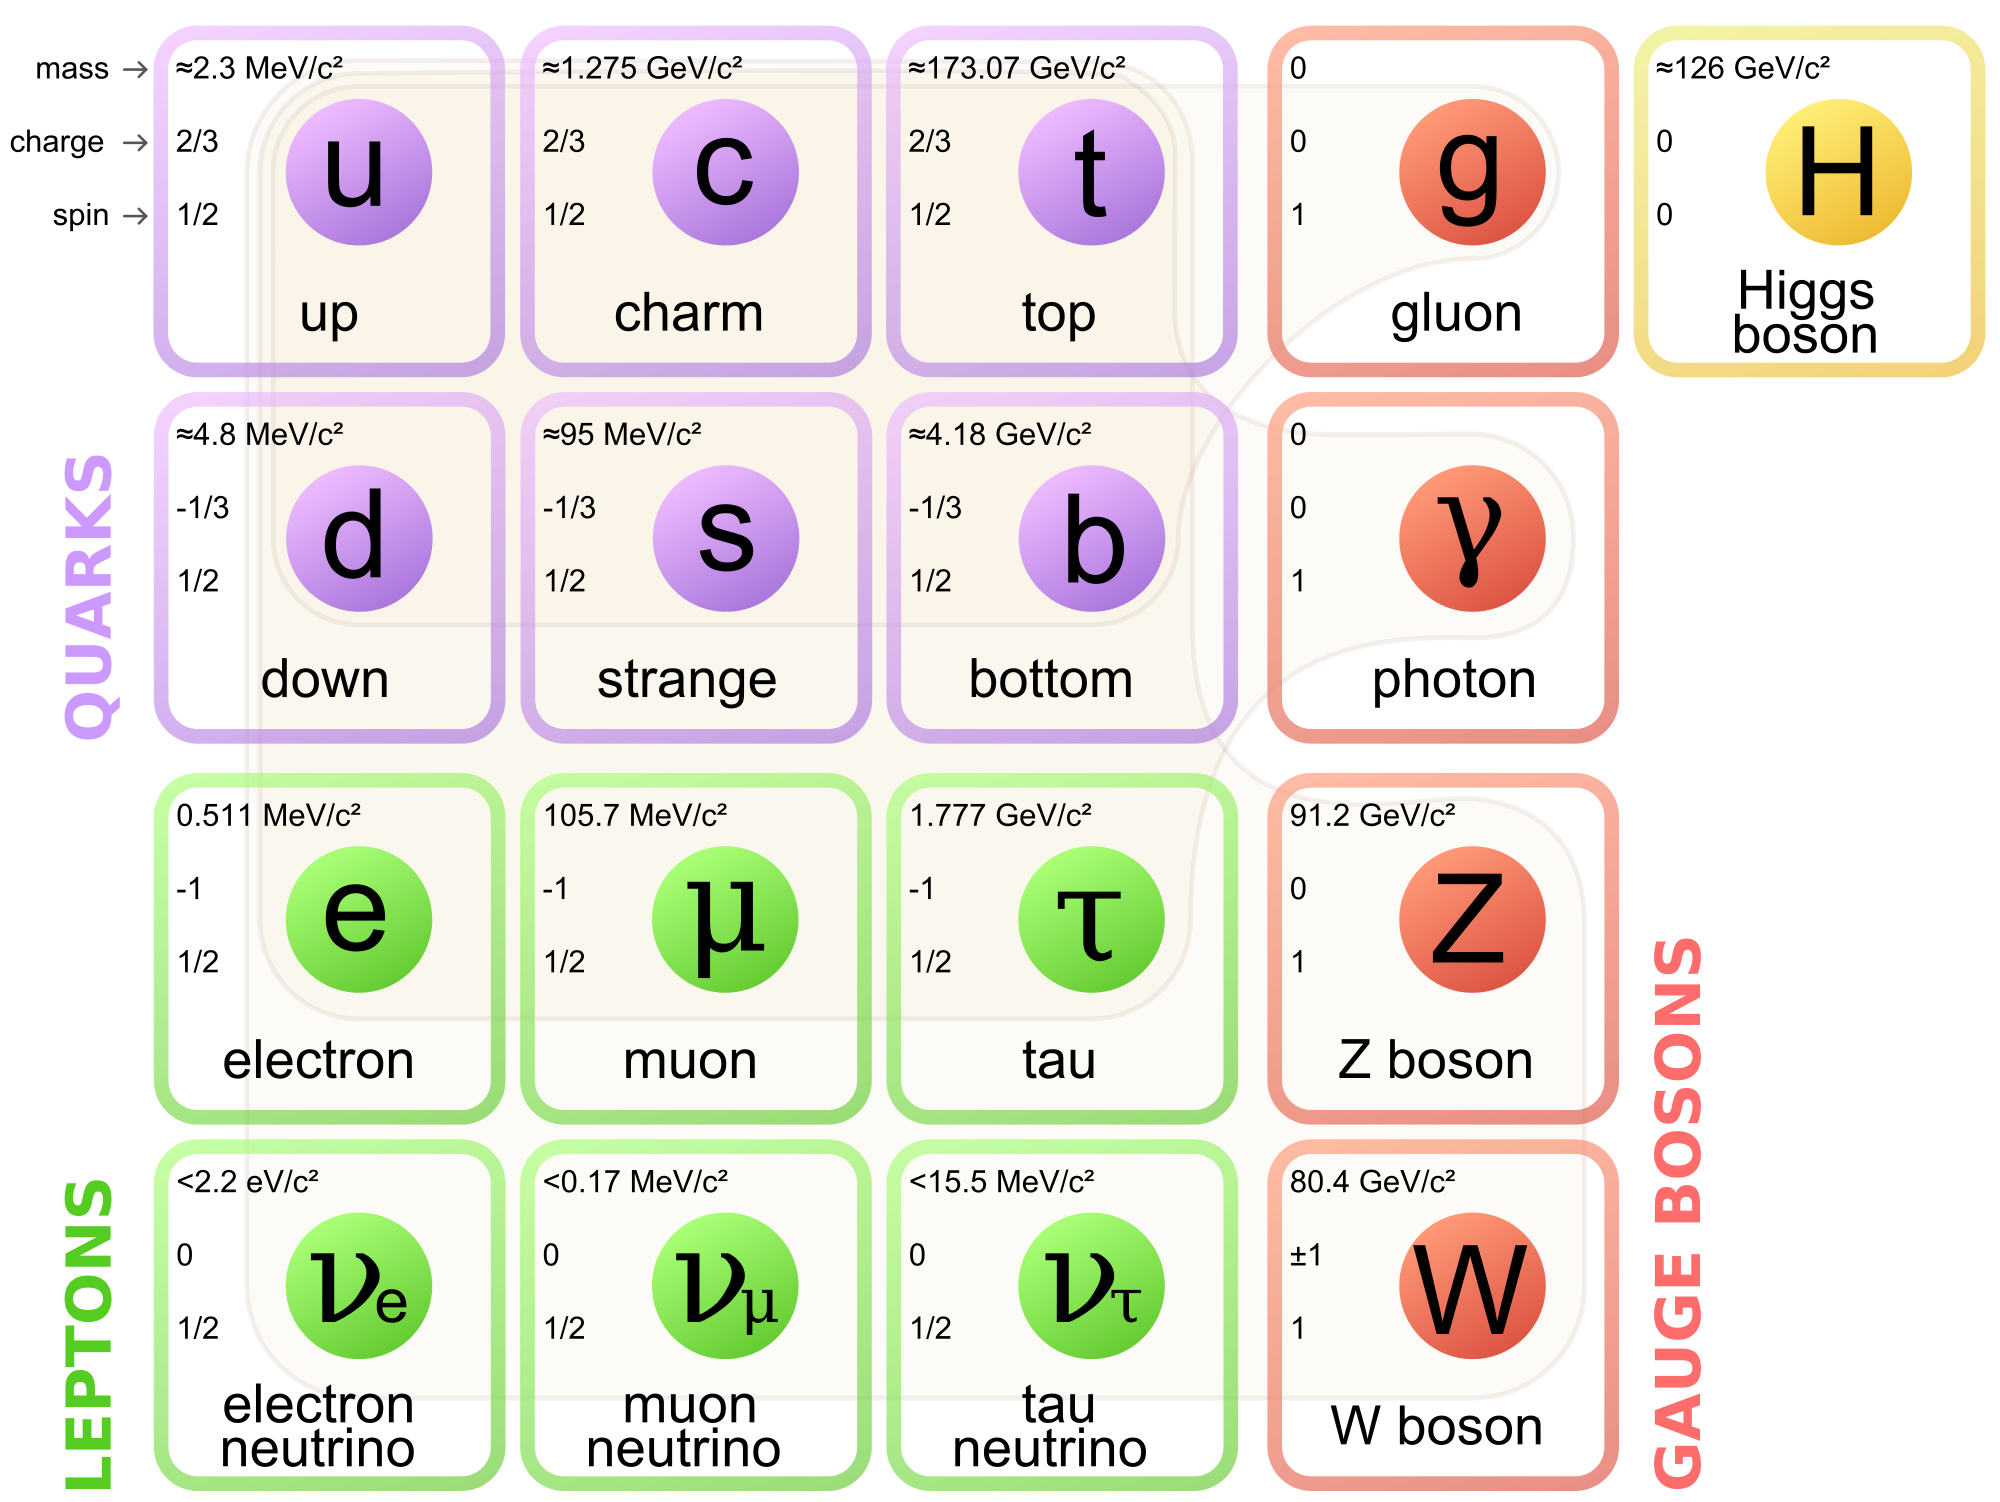
\includegraphics[width=0.6\textwidth]{01_Theory_SM/plots/Standard_Model_of_Elementary_Particles.png}
  \caption{The Standard Model of Elementary Particle Physics with three generations of matter fermions, gauge bosons and a Higgs boson. 
  The properties of the particles are also shown in each box. Figure taken from \cite{WikiSM}}
  \label{fig:SM_Particles}
\end{figure}


\subsection{Leptons}

The two bottom rows of fermions in the Fig.\ref{fig:SM_Particles} represent the known \textit{leptons} with their masses, charges
and spins. 

In general, the fermions are described with the Dirac equation\cite{diraceq}, which has 
% \begin{equation}\label{eq:dirac}
%   i\hbar\gamma^{\mu}\partial_{\mu}\psi - mc\psi = 0 ,
% \end{equation}
% 
% where the $\psi$ is a four-element Dirac spinor, an equivalent of a one dimentional Schr\"{o}dinger wave function, 
% $\gamma^{\mu}$s are the gamma matricies and $\partial_{\mu}$ is a partial derivative with respect to the time-space four-vector
% components. 
% 
solutions with positive and also with negative energy states. The latter are treated
as \textit{antiparticles}. So every lepton, being a fermion, has an antiparticle. In Fig.\ref{fig:SM_Particles}
only particles are shown. The electron $e^{-}$ has an antiparticle, called positron $e^{+}$. The antiparticle of the muon -- $\mu^{+}$ --
and tauon -- $\tau^{+}$ -- don't have any special name. As far as we know,
the electron is a stable particle. The muon $\mu^{-}$ and tauon $\tau^{-}$ differ from the electron by their masses and their 
finite lifetimes. Neutral leptons, neutrinos $\nu$, also have antiparticles, antineutrinos $\bar{\nu}$. 

Leptons are grouped into families and each lepton family has a corresponding lepton number: an electron and an electron neutrino 
have a lepton number $l_{e}$, the muon and it's neutrino have a lepton number $l_{\mu}$ and the $\tau$ with it's neutrino have the 
lepton number $l_{\tau}$.  Leptons have positive lepton numbers and antileptons -- negative ones.
% The lepton number is
% conserved during the interactions.

\subsection{Quarks}\label{sec:quark}

The two upper rows in the Fig.\ref{fig:SM_Particles} list the known \textit{quarks}, showing their masses, charges and spins.

Quarks are also fermions. However, there is a number of properties which are very different
to the leptons. They have  a \textit{flavour} (up, down, charm, strange, top and bottom) and a non-integer electric charge 
($\frac{2}{3} e$ or $-\frac{1}{3} e$, where $e$ is the electron charge).
Quarks also have a charge called \textit{color}. 
% All the observed isolated objects can't have color, they are colorless. Thus, the 
% quarks have never been observed in an isolated state. 

The systems of bound quarks are called \textit{hadrons}. The examples of such systems are 
\textit{baryons}, which consist of three quarks, and \textit{mesons}, which consist of a quark and antiquark. The only stable yet known baryon 
is the proton. All the known mesons are unstable.

The baryons are fermions as they consist of an odd number of quarks which have spins $\frac{1}{2}$. The mesons have integer spins
(0 or 1). This means that mesons are bosons.

\section{Interactions}

An interaction is the way the particles effect upon another particles and objects in their environment. The interaction is performed through exchange
of mediator bosons.

Nowadays only four basic interactions are known: \textit{strong}, \textit{electromagnetic}, \textit{weak} and \textit{gravity}. 
Each of them can be characterized by a \textit{strength}\footnote{A $strength$\cite{griffiths2008introduction} of the four basic forces can be determined as the value of each force
between two objects with given masses and charges and placed on a distance $r$ between each other. After all, the strength is an ambiguous notion, as the 
value of the force depends on the nature of the interacting objects and on the distance between them -- we can get different orders of strength on different
distances  and between different objects. The strength should not be understood literally, but just as a measure of order.}.
The following table shows the rough order of the interaction strengths, the mediator
and the theory, which describes these interactions \cite{griffiths2008introduction}:

\begin{center}\label{tab:forces}
  \begin{tabular}{ | c | c | c | c | }
    \hline
    \textbf{Interaction} & \textbf{Strength} & \textbf{Theory} & \textbf{Mediator} \\ \hline \hline
    Strong & 10 & Quantum Chromodynamics & Gluon \\ \hline 
    Electromagnetic & 10$^{-2}$ & Quantum Electrodynamics & Photon \\ \hline
    Weak & 10$^{-13}$ & Flavordynamics & $W$ and $Z$ Bosons \\ \hline
    Gravitation & 10$^{-42}$ & Geometrodynamics & Graviton \\
    \hline
  \end{tabular}
\end{center}

All the equations and values listed in this work are presented assuming that $\hbar = c = 1$. This is called the \textit{natural units}. 
More details on every interaction is presented in the following section.

\subsection{Electromagnetic Interaction}

The theory behind the electromagnetic interactions -- quantum electrodynamics (QED) \cite{PhysRev.75.486} -- was developed earlier than the other 
interactions quantum theories. It describes the interactions between the elementary electrically charged fermions via mediator photons.
The electromagnetic interaction is such that the oppositely electrically charged objects attract each other while same sign charges repulse.
This interaction is present at any distance, getting weaker proportionally to the distance squared. QED is based on the gauge group $U(1)$.
Every electromagnetic phenomena is ultimately reducible to the following elementary process:

\begin{figure}[h]
  \centering
  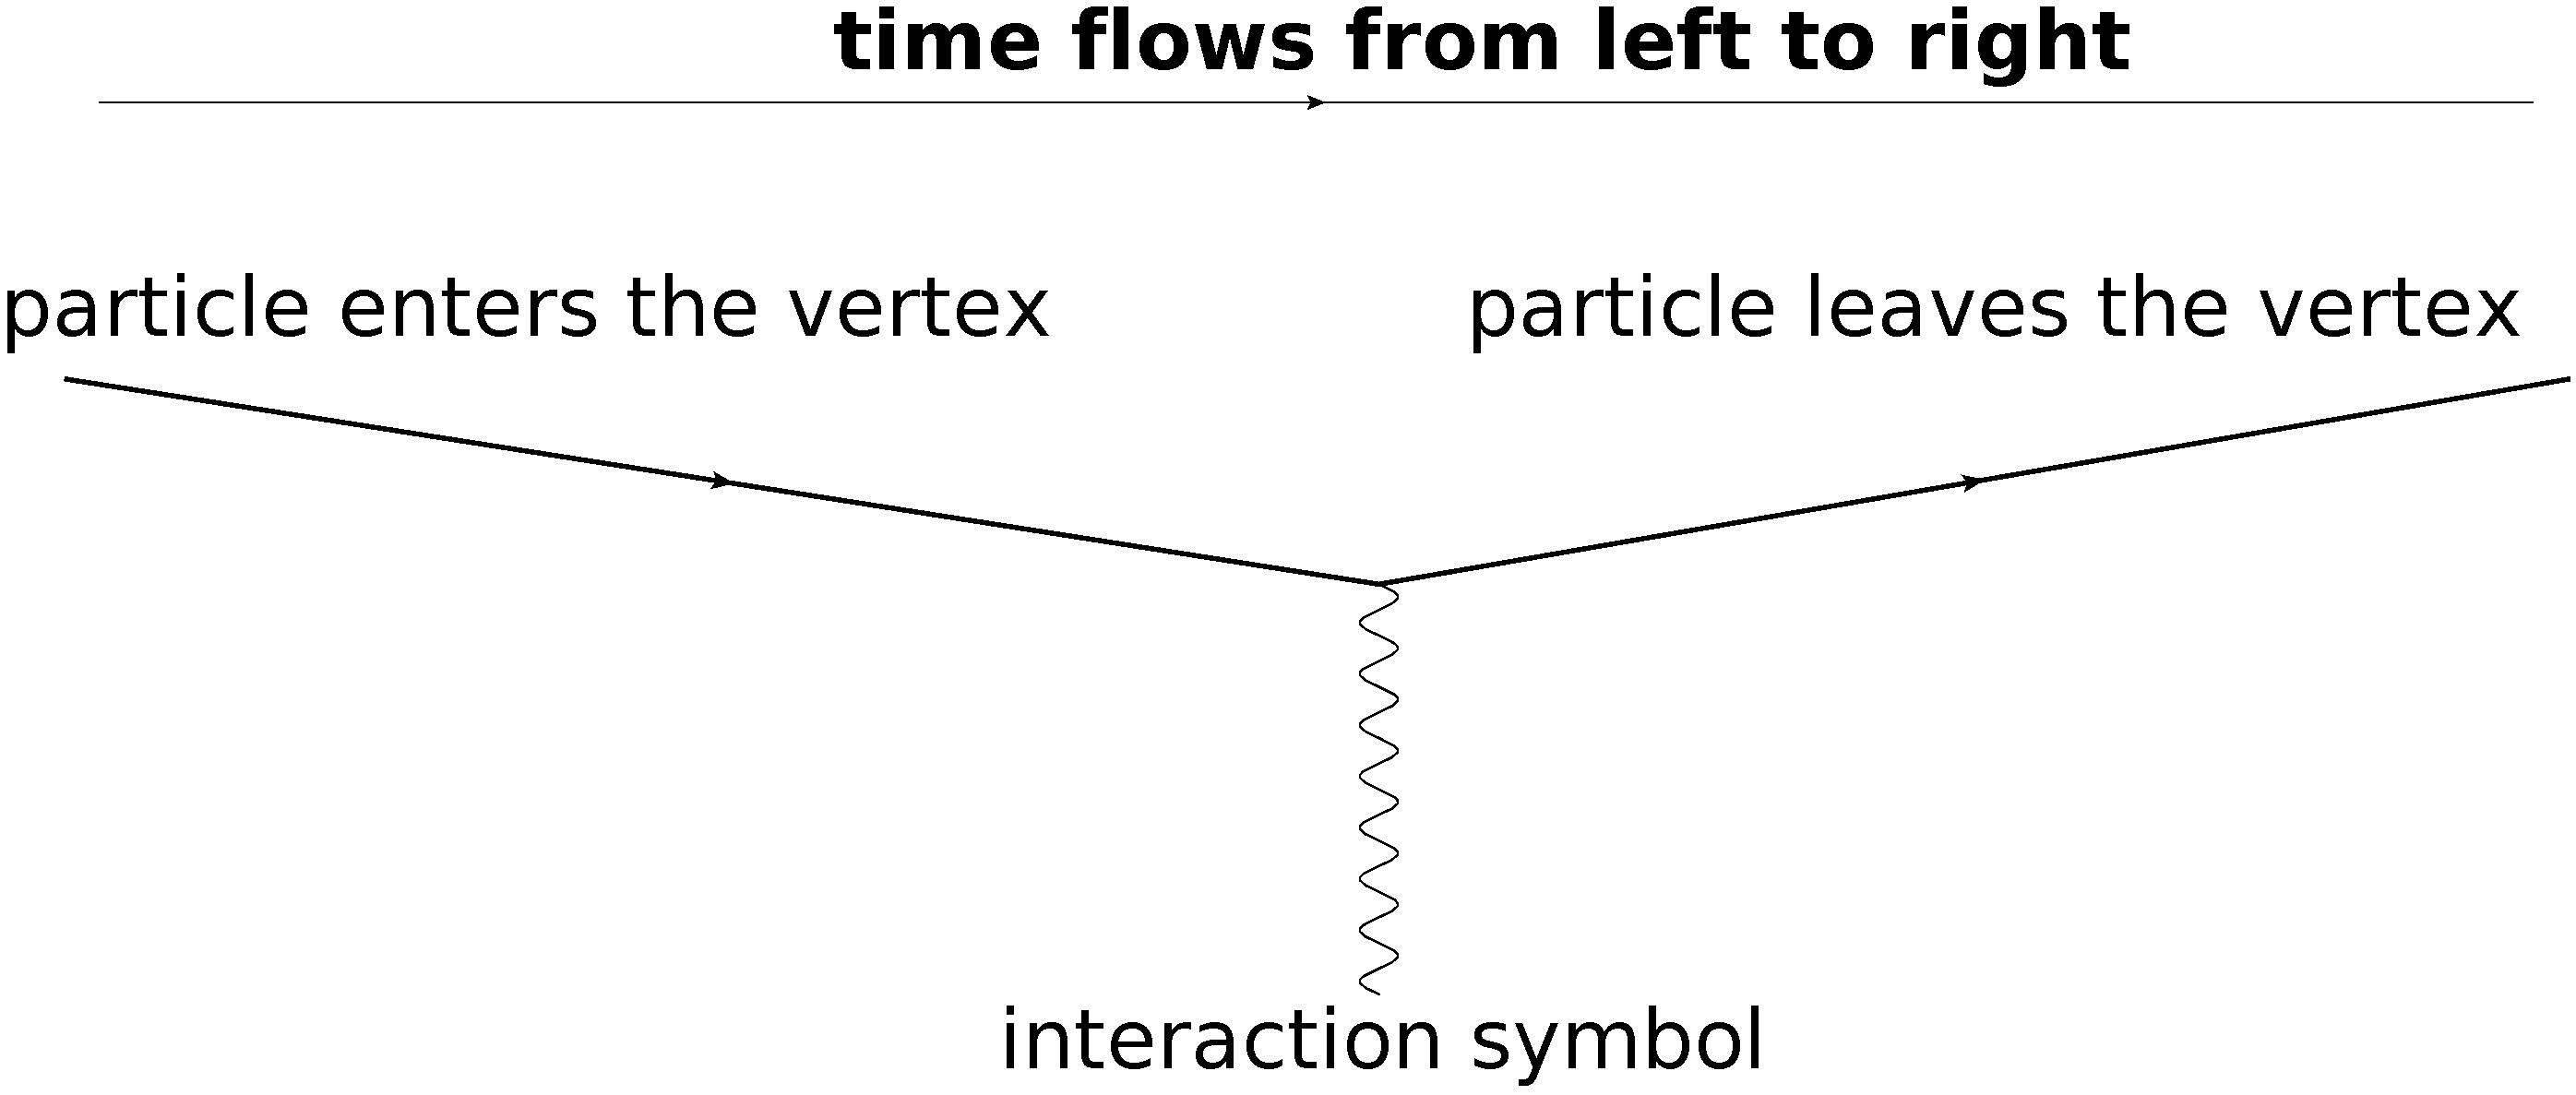
\includegraphics[width=0.6\textwidth]{01_Theory_SM/plots/QED_simple_uniform.png}
  \caption{Feynman graph of the elementary QED process.}
  \label{fig:QED_simple}
\end{figure}

The more complex processes can be described combining two or more of these elementary vertices.

The coupling constant, or the interaction strength of the electromagnetic interaction is given as following:

\begin{equation}
 \alpha = \frac{e^{2}}{4\pi\epsilon_{0}} \approx \frac{1}{137},
\end{equation}

where $\epsilon_{0}$ is the permitivity of vacuum and $e$ is the electron charge.

As the coupling constant is small ($\alpha \ll 1$), it can be used for expansion in perturbative calculations (observable $\sim\sum_{k=0}^{\infty} c_{k}\cdot\alpha^{k}$).
The naming of the processes, described by each of the terms of the $\alpha$ expansion
is Leading Order process (LO, which takes into account the first term with non-zero $c_{k}$), Next-to-Leading Order process (NLO, also takes
to account the next term, additionally to the LO), Next-to-Next-to-Leading Order process (NNLO), etc.

\subsection{Strong Interaction}\label{sec:strong_int}

The theory which describes the strong interaction is Quantum Chromodynamics (QCD), which is based on the gauge group $SU(3)$. Only the
objects which have a color charge can interact strongly. The color charge (first mentioned in sec. \ref{sec:quark}) has three eigenstates:
red (r), blue (b) and green (g). As for any other charge, the color charge eigenstates have also anticharges -- anticolors. The combination
of the color and corresponding anticolor, as well as the combination of all the colors/anticolors results in colorless states.

The mediators of the strong interaction are gluons. These particles are massless and carry two colors -- color and anticolor. The strong 
interaction is the interaction between quarks and gluons via gluons. The color charge is conserved during the interaction.

The coupling constant of the strong interaction, $\alpha_{s}$, is depending on the energy scale $Q$. As shown in the
Fig. \ref{fig:Alpha_s}, $\alpha_{s}$ rapidly increases with decreasing $Q$. This means that at larger distances 
the strength of the interaction increases a lot. This phenomenon is called \textit{confinement} and this means that the quarks
can't exist in an isolated state. The more the quarks separate from each other in terms of distance, the stronger they interact, the harder
it becomes to separate them further. Even if enough energy is present to separate quarks more and more from each other, the gluon field will become critically
high and produce a quark-antiquark pair out of the vacuum. This process may repeat sequentially. 
% This constantly happens under the conditions created in
% particle colliders. 
The phenomenon of sequential quark pair production is called \textit{hadronization}.

The confinement constrains the maximum distances on which the interaction in terms of the gluon field is observed before producing a quark-antiquark pair.
The limit of the region of strong interaction impact is of the order of the nucleon size $\sim 10^{-15}$ m.

\begin{figure}[t]
  \centering
  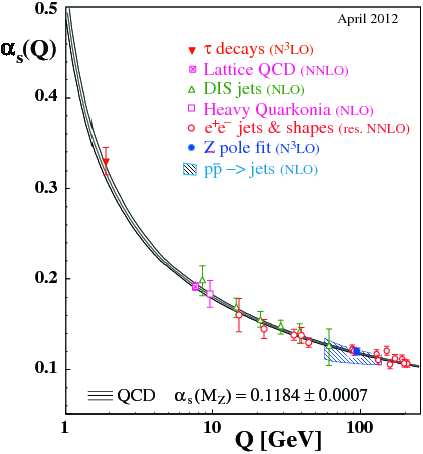
\includegraphics[width=0.6\textwidth]{01_Theory_SM/plots/Alpha_s.png}
  \caption{Summary of measurements of $\alpha_s$ as a function of the respective energy scale $Q$. The respective degree of QCD perturbation 
  theory used in the extraction of $\alpha_{s}$ is indicated in brackets (NLO: next-to-leading order; NNLO: next-to-next-to leading order; 
  res. NNLO: NNLO matched with resummed next-to-leading logs; N3LO: next-to-NNLO). Figure taken from \cite{PDG-2012}.}
  \label{fig:Alpha_s}
\end{figure}

The opposite tendency which can be observed in Fig. \ref{fig:Alpha_s} is that the $\alpha_{s}$ is getting smaller for higher values 
of the $Q$. This means that for the shorter interaction distances, the coupling constant becomes weaker. This phenomenon carries the 
name \textit{asymptotic freedom}\cite{PhysRevLett.30.1343}. Under these conditions the quarks can be effectively treated as free particles. The asymptotically 
free quarks are assumed to be observed in the \textit{quark-gluon plasma} \cite{Bohr1977275} -- the state of matter with extremely high density and/or temperature.

% The conjectured QCD states, depending on temperature and density, are shown in Fig. \ref{fig:QGP}.

% \begin{figure}[t]
%   \centering
%   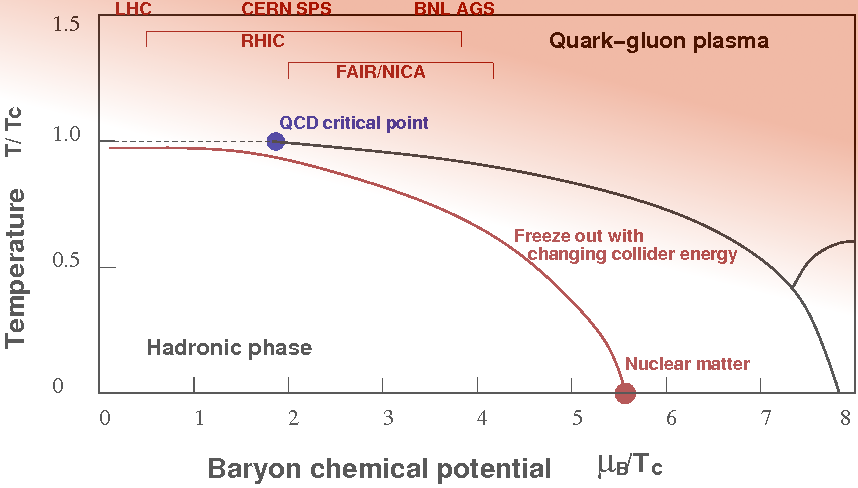
\includegraphics[width=0.8\textwidth]{01_Theory_SM/plots/QGP.png}
%   \caption{Conjectured phase diagram of QCD. The different states and phase curves are shown. The energy and density range of different high energy 
%   physics experiments are marked on the top of the figure.}
%   \label{fig:QGP}
% \end{figure}

\subsection{Weak Interaction}

As it can be seen in the table \ref{tab:forces}, the strength of the weak interaction is many orders of magnitude smaller than the one for the 
electromagnetic and strong interaction. This fact explains the name \textit{weak}.

A charge, which is responsible for the weak interaction is the \textit{weak isospin} $I_{3}$. All the left-handed\footnote{The 
\textit{chirality} of the particle defines it's handnessness. The left-handed and right-handed states are different components of the Dirac spinor\cite{aitchison2003gauge}. 
The parity transformation change the chirality (from left-handed to right handed and vise versa). For massless particles chirality is the same as helicity 
-- the property of the particle, which describes the coincidence of the spin and motion directions.} leptons and quarks carry the ability to interact
weakly.
% The weak interaction differs from the others in a way that there is no particular name for the charge responsible for this interaction 
% (like electrical charge for the electromagnetism and color charge for the strong interaction). 
A widely known example of the weak interaction is the process of the $\beta$-decay. The lepton number and lepton flavour both conserve in the weak interaction.

There are two kinds of weak interaction: \textit{neutral}, mediated by the 
$Z$-bosons, and \textit{charged}, mediated by the $W^{\pm}$. The masses of the 
mediators are shown in the Fig. \ref{fig:SM_Particles}.	In the neutral weak interaction there is no electric charge as well as no quark flavour exchange between the 
interacting particles. In the charged weak interaction, both the electric charge and the quark flavour exchange, are present.  
In the charged weak interactions the quark flavour can exchange not only within one generation, but also between the generations.
This intergeneration flavour exchange is described the following way. 
\begin{equation}
\left( \begin{array}{c}
       u \\ d
      \end{array} \right)
\left( \begin{array}{c}
       c \\ s
      \end{array} \right)
\left( \begin{array}{c}
       t \\ b
      \end{array} \right)
\end{equation}
These are the quark mass eigenstates. The weak quark eigenstates differ from the mass eigenstates. For the former ones, the $d$, $s$ and $t$ states are replaced with 
their linear combinations $d'$, $s'$ and $b'$, expressed as follows:

\begin{equation} \label{eq:CKM_transform}
\left( \begin{array}{c} d' \\ s' \\ b' \end{array} \right) = 
\left( \begin{array}{ccc} V_{ud} & V_{us} & V_{ub} \\ V_{cd} & V_{cs} & V_{cb} \\ V_{td} & V_{ts} & V_{tb} \end{array} \right)
\left( \begin{array}{c} d \\ s \\ b\end{array} \right).
\end{equation}

The matrix $V$ in \ref{eq:CKM_transform} is the Cabibbo-Kobayashi-Maskawa matrix (CKM-matrix)\cite{Kobayashi:1973fv}, which describes the transition probability 
between different quark flavours. Experimentally defined, the matrix elements have the following magnitudes \cite{PDG-2012}:

\begin{equation} \label{eq:CKM}
 V = \left( \begin{array}{ccc} 0.974 & 0.225 & 0.003 \\ 0.225 & 0.973 & 0.041 \\ 0.009 & 0.040 & 0.999 \end{array} \right).
\end{equation}

The diagonal elements of the CKM matrix (\ref{eq:CKM}) are close to 1, being much larger than the off-diagonal elements. Thus, flavour transformations
within one generation are preferred.

As the masses of the gauge bosons which mediate the weak interaction are quite large (see Fig. \ref{fig:SM_Particles}), the range of the interaction is restricted
to a size of $\sim \frac{1}{M_{W}}$, where $M_{W}$ is the mass of the $W^{\pm}$ boson, 80.4 GeV.

\subsection{Electroweak Unification and Symmetry Breaking}

If one compares the neutral weak interactions and the electromagnetic ones, it becomes obvious that they are very similar, differing mainly on the mediator
of the interaction. This can be also seen in Fig. \ref{fig:em_weak}.

\begin{figure}[h]
  \centering
  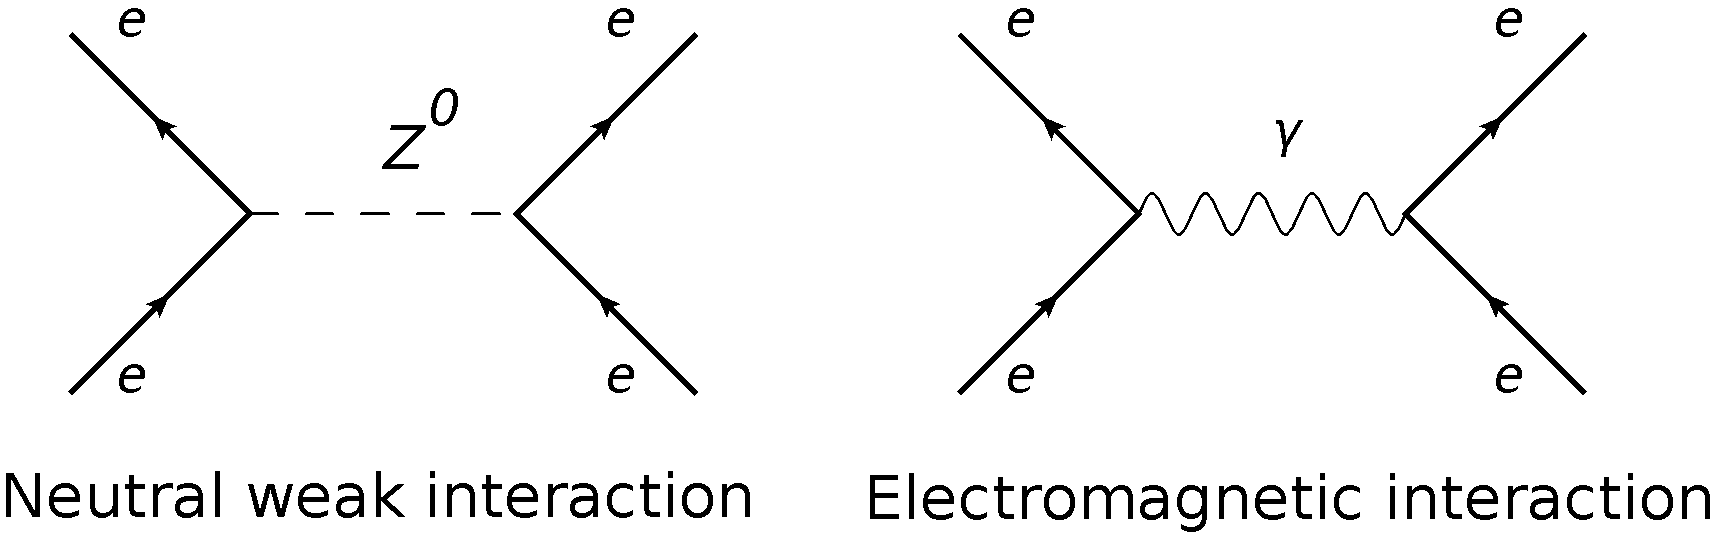
\includegraphics[width=0.6\textwidth]{01_Theory_SM/plots/feynz_uniform.png}
  \caption{$e^{+}e^{-}$ scattering in the electromagnetic (right) and neutral weak (left) interactions.}
  \label{fig:em_weak}
\end{figure}

A unification of these two interactions would seem to be a natural idea. It is not that simple as replacing the $Z^{0}$ by the photon $\gamma$, one
should take to account both processes and their interferences.

The theory \cite{Bilenky:1982ms} which describes the unified electroweak interactions is based on the $SU(2) \times U(1)$ symmetry. To make the Lagrangian of the weak interaction
symmetric to the $SU(2)$ transformations, three fields are introduced: $W_{\mu}^{1}$, $W_{\mu}^{2}$ and $W_{\mu}^{3}$. These fields couple to fermions with
the coupling constant $g$. The fields $W_{\mu}^{1}$ and $W_{\mu}^{2}$ couple to the left-handed fermions and
the $W_{\mu}^{3}$ is coupling to the neutrinos. The $W^{\pm}$ couples to the left-handed fermions, thus it can be represented as a linear combination of
$W_{\mu}^{1}$ and $W_{\mu}^{2}$:

\begin{equation}
 W^{\pm} = \frac{1}{\sqrt{2}}(W_{\mu}^{1} \mp iW_{\mu}^{2}).
\end{equation}

The symmetry $U(1)$ introduces the additional field $B_{\mu}$ which couples to neutrinos. The related coupling constant is $g'$. To describe the electromagnetic
field, the $Z_{\mu}$ and $\gamma_{\mu}$ fields are introduced:

\begin{equation}\label{eq:Zmu}
 Z_{\mu} = \frac{1}{\sqrt{g^{2} + g'^{2}}}(gW^{3}_{\mu} - g'B_{\mu}),
\end{equation}

\begin{equation}\label{eq:Amu}
 \gamma_{\mu} = \frac{1}{\sqrt{g^{2} + g'^{2}}}(gW^{3}_{\mu} + g'B_{\mu}).
\end{equation}

A free parameter of the Standard Model, which is introduced in this context, is the weak mixing angle $\theta_{W}$, which is expressed as follows:

\begin{equation}
 \cos(\theta_{W}) = \frac{g}{\sqrt{g^{2}+g'^{2}}}.
\end{equation}

Thus, the fields $Z_{\mu}$ and $\gamma_{\mu}$ can be expressed via this angle:

\begin{equation}
 Z_{\mu} = W^{3}_{\mu}\cos(\theta_{W}) - B_{\mu}\sin(\theta_{W}),
\end{equation}

\begin{equation}
 \gamma_{\mu} = W^{3}_{\mu}\cos(\theta_{W}) + B_{\mu}\sin(\theta_{W}).
\end{equation}

So in fact, the photon $\gamma$ and the $Z^{0}$ mix the states of $W^{3}_{\mu}$ (corresponding to $W^{0}$) and $B_{\mu}$ (corresponding to $B^{0}$).
The mixing angle $\theta_{W}$ has been measured experimentally \cite{PDG-2012} and corresponds to approximately $30^{o}$.

There is also a charge introduced to describe the electroweak interaction, which is called a \textit{hypercharge} $Y$ and is expressed in the Gell-Mann--Nishijima
equation:

\begin{equation}
 Y = (2Q - I_{3}).
\end{equation}Here $Q$ is an electric charge in units of the electron charge $e$ and $I_{3}$ is the weak isospin.

The whole model, however, is based on the assumption that all gauge bosons have to be massless, which is not the case. The known experimental fact
is that the $W^{\pm}$ and $Z^{0}$ bosons carry a non-zero mass \cite{PDG-2012}. The masses appear in this theory due to \textit{spontaneous gauge symmetry
breaking}. In another words, the particles remain massless, but a new field appears. The particles couple to this field and obtain masses in this
interaction. The symmetry breaking is accompanied with the appearance of three massless particles with zero spin, so-called \textit{Goldstone bosons}.
They are eliminated by the \textit{Higgs mechanism}\cite{1964PhRvL..13..508H}, which, however, introduces a massive particle with zero spin - \textit{Higgs boson}. At the time when the
Higgs mechanism was introduced, such particle was not yet discovered. A Higgs-like particle was discovered only in 2012 \cite{Aad20121, Chatrchyan:2012xdj} 
and it's properties still need to be checked for the consistency to the theoretical predictions.


\subsection{Gravity}

The fourth interaction which is present in our Universe is gravity. The gravity is not described in the Standard Model, but it has to be mentioned for a consistent 
picture. The gravity is described by the \textit{general relativity}, which is a classical non-quantum field theory. Up to now it couldn't be combined with the
Standard Model. The Standard Model breaks down at the large scale, where gravity starts to play role. Although the extension of the Standard Model is predicting 
the existence of a gravity gauge boson -- a \textit{graviton} with a spin 2 and zero mass -- there has been no experimental proof of it's existence to date.
The "charge`` which reacts to the gravity is the mass of the interacting object.

The gravitation force between the elementary particles is very weak, even though the distances are very small (the gravity strength is proportional to $\sim\frac{1}{r^{2}}$). 
The reason for that are very low masses of the interacting particles. Gravity only becomes noticable
on large distances when large, electrically uncharged objects with large masses are interacting. For example, the movement of the bodies in outer space 
(planets, stars, asteroids, etc) are to the large extend governed by gravity. 

The influence of gravity is negligible for the processes studied in this thesis, thus it is neglected.

\section{Top Quark Physics}

In this thesis the process of $t\bar{t}$ production is being analyzed. Some more details of the top quark physics should be presented.
The top quark has unique properties compared to the other elementary particles: it is the heaviest known elementary particles and its mass is so large that its the lifetime 
is smaller than the typical hadronization time. Thus, the top quark decays 
faster than it can hadronize, which means that studying the top quark is gaining knowledge about a bare quark. This section describes the production process of the top quark and its decay.

\subsection{Top Quark Production}\label{ssec:tprod}

The top quark production cross section depends on the center-of-mass energy of the experiment in which it is produced. From Fig. \ref{fig:SM_XSec_Prod}
one can judge that the LHC with its large center-of-mass energy (design energy of 14 TeV) acts like 
a top production factory. The top production cross section ($\sigma_{top}$) at the LHC scale is almost an order of magnitude larger than for the
TEVATRON.

\begin{figure}[p]
  \centering
  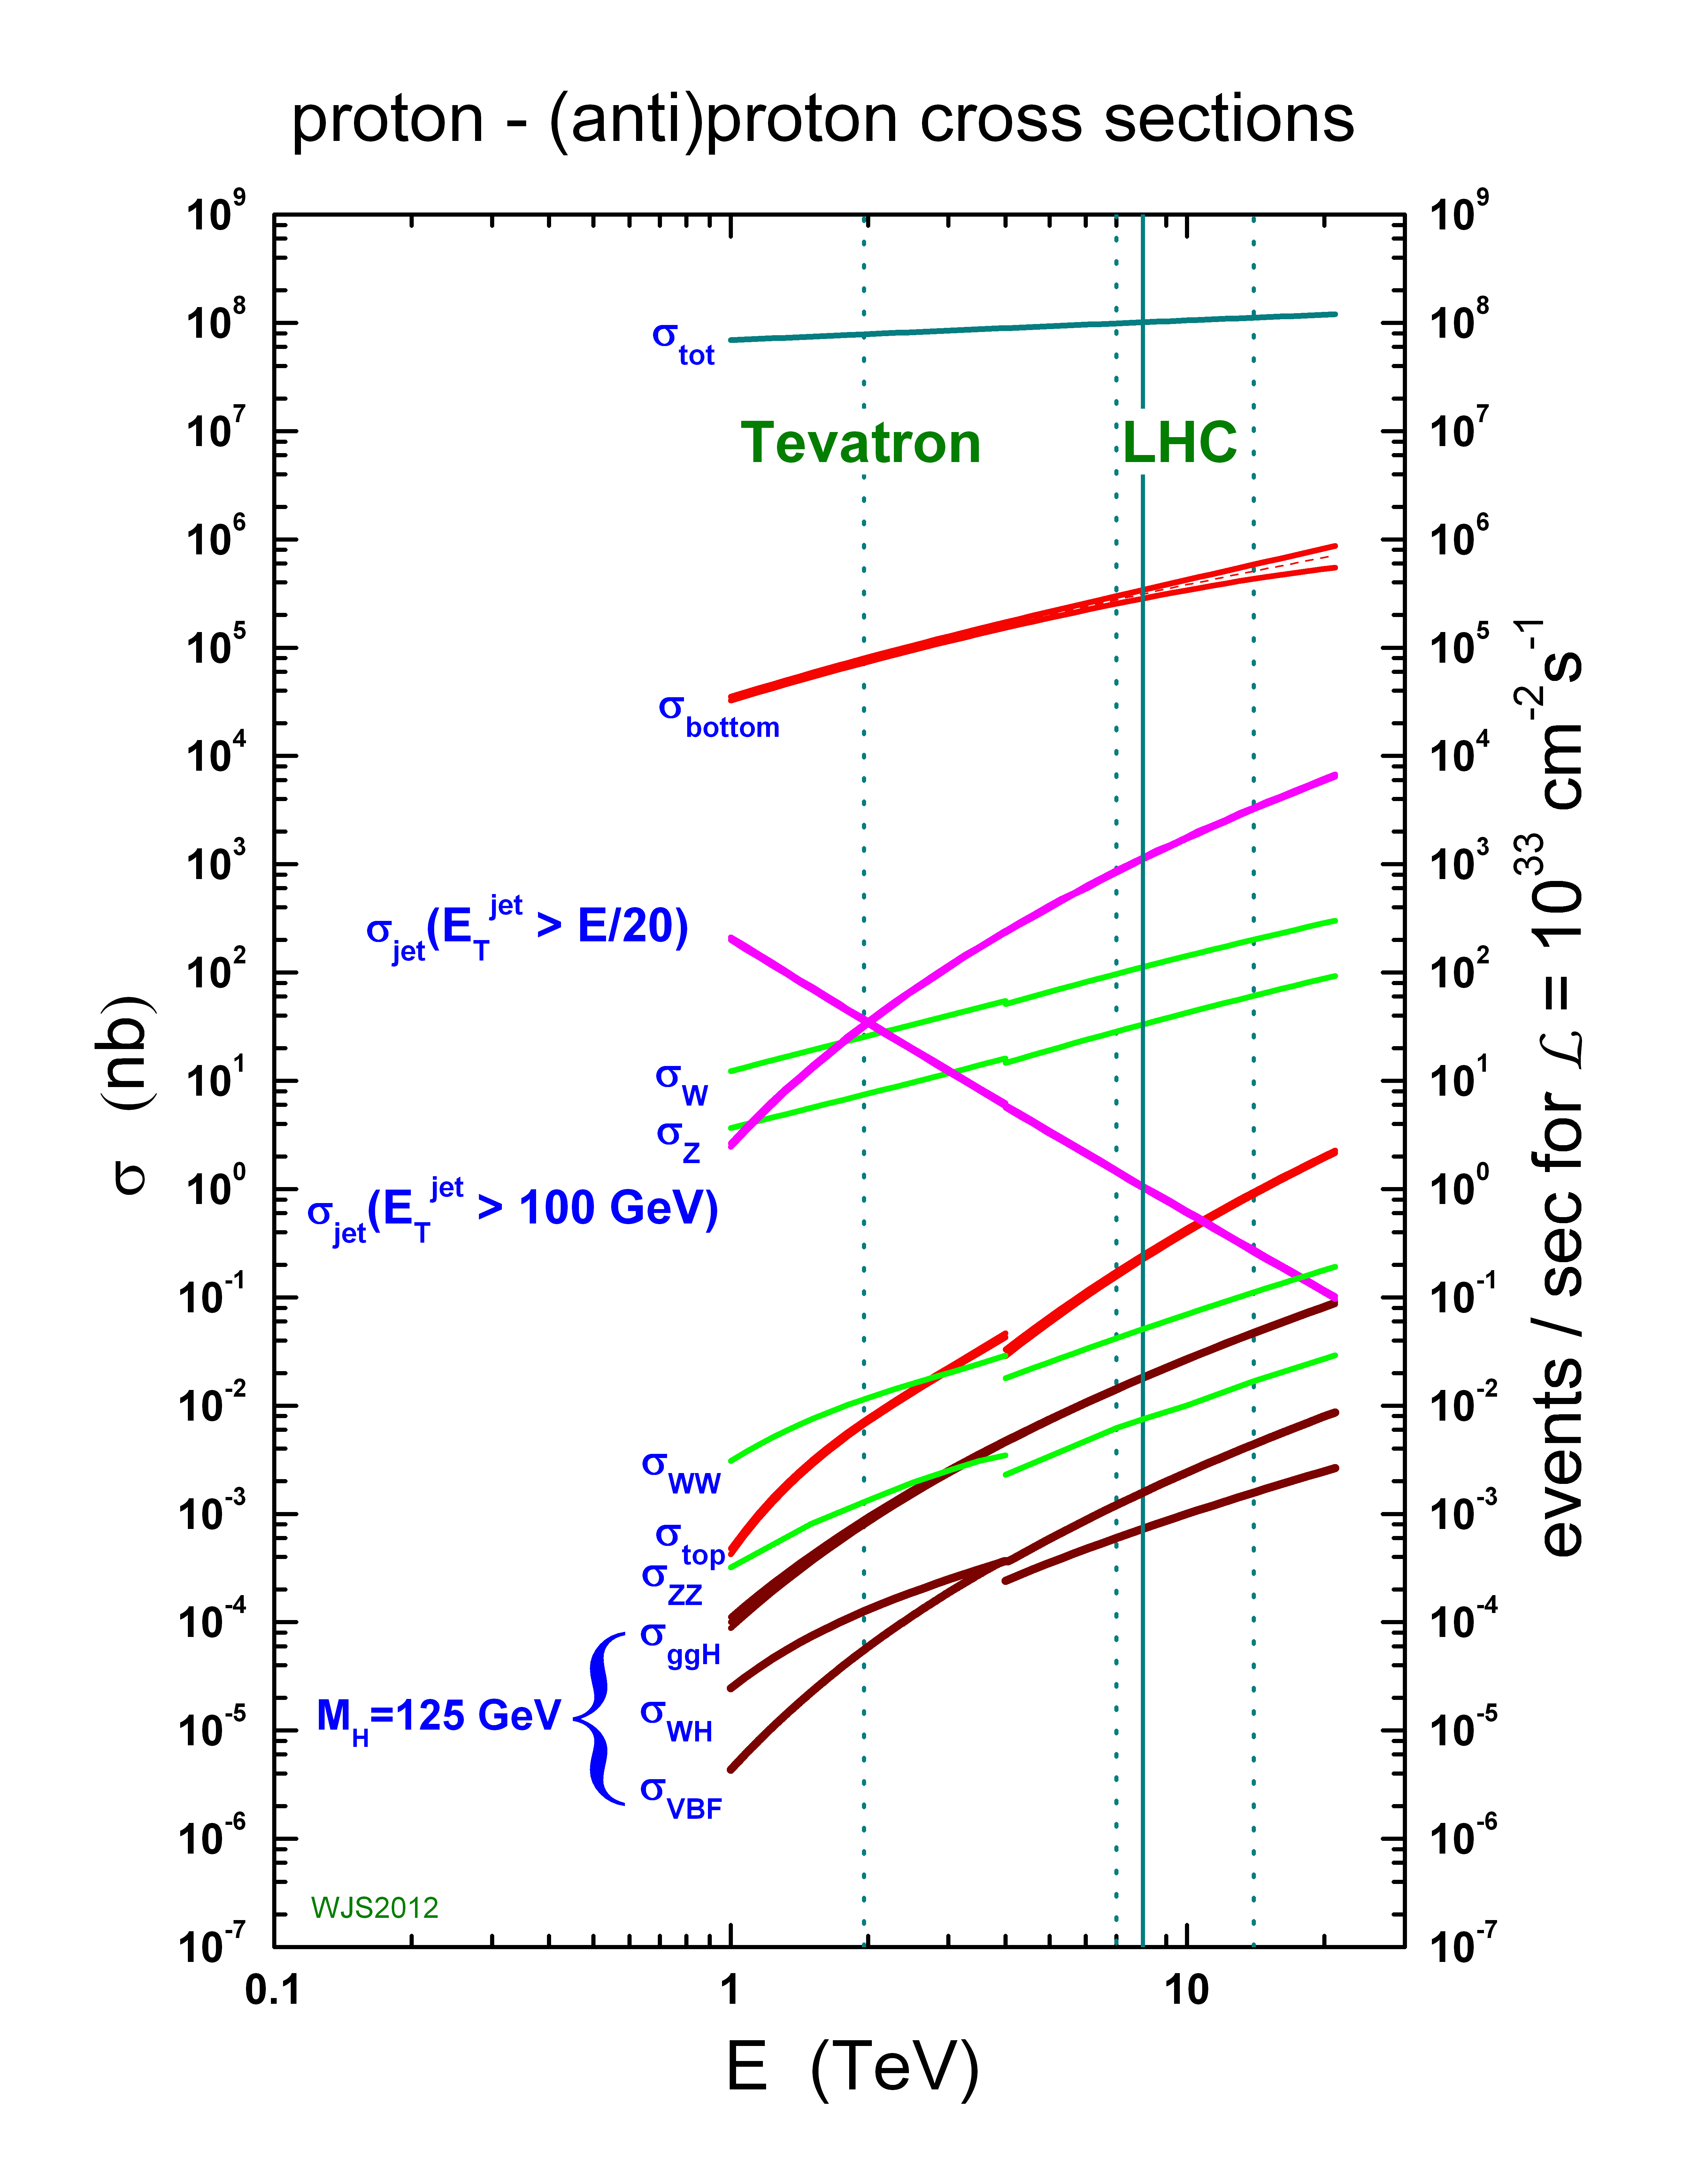
\includegraphics[width=1.0\textwidth]{01_Theory_SM/plots/crosssections2013.png}
  \caption{Standard Model leading order cross sections for different SM processes depending on the energies. The turquoise vertical line presents the energy
  of the Large Hadron Collider running in 2012. The plot is taken from \cite{Stirling}.}
  \label{fig:SM_XSec_Prod}
\end{figure}

The top quarks may be produced as single top quarks or in pairs.

\subsubsection{Single Top Production}

Single top quarks can be produced in the weak interaction processes via the $Wtb$ vertex.

There are three production modes of the single top -- $t$-channel, $s$-channel and $tW$-channel. These production channels are shown in Fig. \ref{fig:single_t_prod}.

\begin{figure}[H]
  \centering
  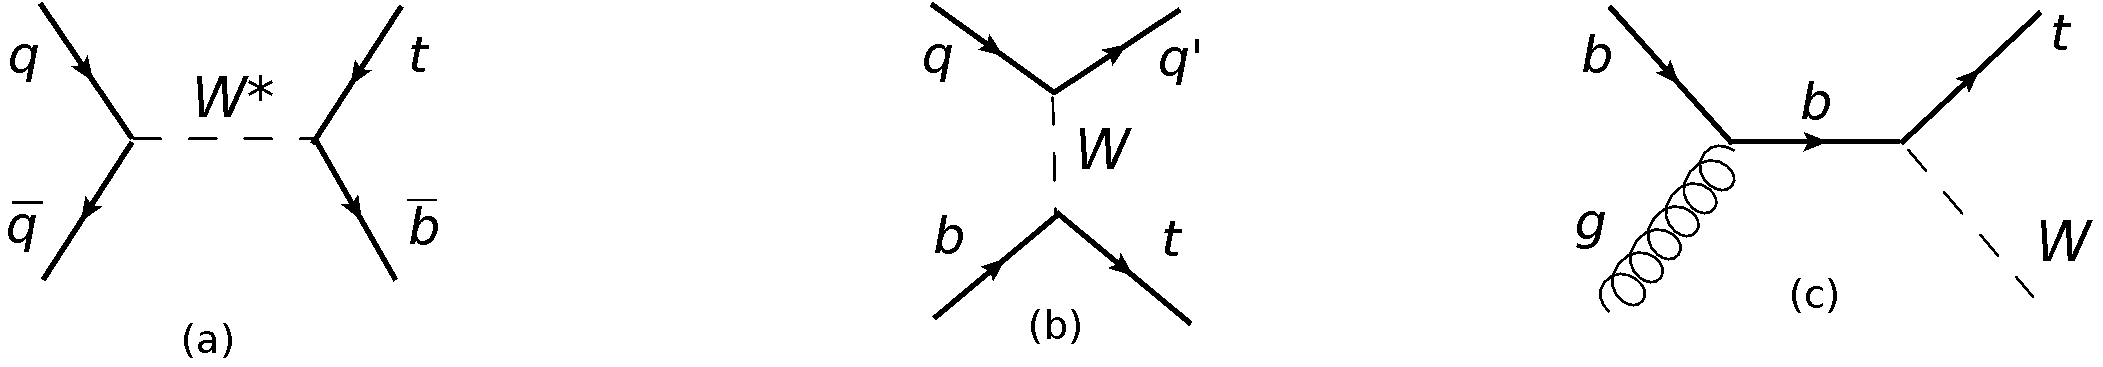
\includegraphics[width=1.0\textwidth]{01_Theory_SM/plots/single_top_uniform.png}
  \caption{Feynman diagrams for the LO single $t$-quark production. Three different production channels for single top quarks are illustrated: 
  the $s$-channel (a), the $t$-channel (b) and the W-associated $tW$-channel (c).}
  \label{fig:single_t_prod}
\end{figure}

Single top quark production is interesting for various studies. It is a test of the Standard Model and it is directly sensitive to the CKM matrix
element $|V_{tb}|$.

\subsubsection{Top Quark Pair Production}\label{ssec:tt_prod}

The dominant SM $t\bar{t}$ production mechanism at the LHC is the gluon-gluon fusion. In QCD the inclusive production cross section of the $t\bar{t}$ pair
from the proton-proton interaction can be factorized as follows \cite{Schilling:2012dx}:

\begin{equation} \label{eq:pptt}
 \sigma_{pp \rightarrow t\bar{t}} (s, m_{t}) = \sum_{i,j = q, \bar{q}, g} \int dx_{i} dx_{j} f_{i}(x_{i}, \mu_{f}^{2}) f_{j}(x_{j}, \mu_{f}^{2}) \cdot \hat{\sigma}_{ij \rightarrow t\bar{t}}(\hat{s}, m_{t}, \mu_{f}, \mu_{r}, \alpha_{s}).
\end{equation}

Here the sum is running over all quarks and gluons contributing to the process, $m_{t}$ is the mass of the top quark, $s$ is the squared center-of-mass 
energy for the $pp$ collision, $x$ is the parton momentum fractions with respect to the proton momenta, $\mu_{f,r}$ are the factorization and renormalization 
scales, $\hat{s} \sim sx_{i}x_{j}$ is the partonic center-of-mass energy, $\alpha_{s}$ is the strong coupling constant and  $f_{i(j)}(x, \mu_{f}^{2})$ is the parton distribution
function (PDF). 

The formula \ref{eq:pptt} is a convolution of long-distance contributions (proton densities) and short distance contributions (hard scattering cross sections). 
As the mass of the $t\bar{t}$ pair is high, the $\alpha_{s}$ turns out
to be quite low (see Fig. \ref{fig:Alpha_s}), thus the perturbative expansion of the hard scattering cross sections is possible -- $\sigma \sim \sum_{k} c_{k}\alpha_{s}^{k}(\mu)$,
where the smallest $k$ defines the leading order. The \textit{Parton Density Function}, or the \textit{PDF}, is depending on the parton flavour $i$, parton momentum
fraction $x_{i}$ and the energy scale of the interaction. A PDF gives a probability that within the interaction of a given scale a parton with a given flavour $i$
and longitudinal momentum fraction $x_{i}$ will be found in a proton. PDFs can't be expanded in perturbative QCD (pQCD), thus need a parametrization, depending on $x$ and 
the scale $Q$. The dependence on the scale $Q$ is described in the DGLAP evolution\cite{Altarelli:1977zs, Dokshitzer:1977sg, Gribov:1972ri}. The scale can be chosen arbitrarily.
%for particular needs.
This scale is called \textit{factorization scale} $\mu_{f}$.
% , it is a sum of the 
% densities of all the quark (valent and from the sea) and gluon constituents. 

The proton densities are obtained as a result of fits to experimental data. 
The PDFs are determined by different groups (for example, HERAfitter \cite{Alekhin:2014irh} or 
CTEQ \cite{Pumplin:2002vw}). The backbone of any modern PDFs are inclusive $ep$ scattering cross sections
measured in deep inelastic $ep$ scattering (DIS) over a wide kinematic range of proton momentum fractions $x$ and hard scales $Q$. 
An example of PDFs obtained by the HERA experiments H1 and ZEUS from fits to their combined inclusive DIS data are shown in Fig. \ref{fig:HERA_PDF}.

\begin{figure}[t]
  \centering
  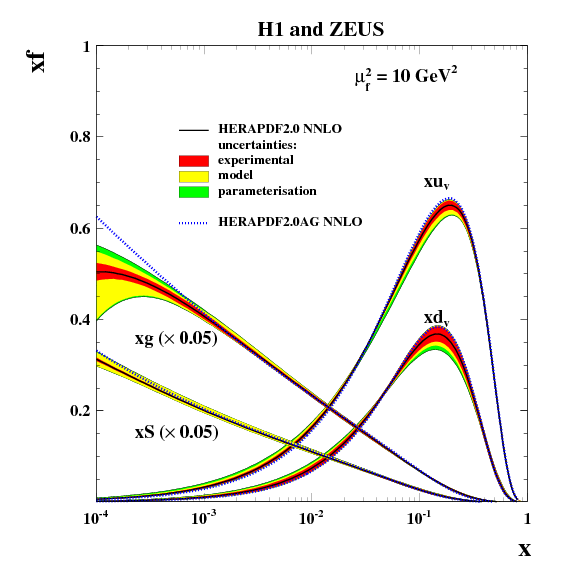
\includegraphics[width=0.8\textwidth]{01_Theory_SM/plots/d15-039f23.png}
  \caption{PDFs from HERAPDF2.0 \cite{Abramowicz:2015mha}.}
  \label{fig:HERA_PDF}
\end{figure}

At the LHC $t\bar{t}$ pairs are dominantly produced in the process of gluon-gluon fusion $gg \rightarrow t\bar{t}$ (at 80\% of the cases at 8 TeV $pp$ collisions) 
and to somewhat lesser extent in quark-antiquark annihilation $q\bar{q} \rightarrow t\bar{t}$ (at 20\% of the cases). These LO production processes are shown in 
Fig. \ref{fig:LO_tt_prod}. In the NLO production processes there are also partonic sub-processes with $gq$($g\bar{q}$) present.

\begin{figure}[h]
  \centering
  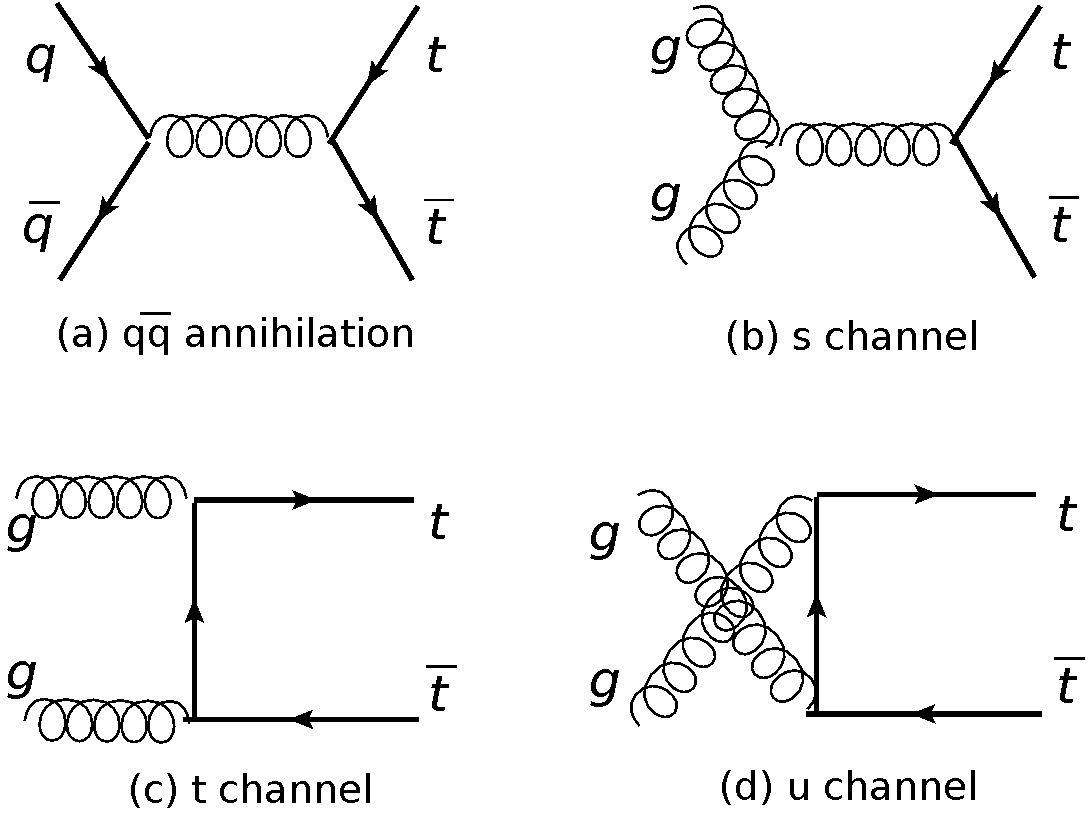
\includegraphics[width=0.8\textwidth]{01_Theory_SM/plots/LO_tt_production_uniform.png}
  \caption{Feynman diagrams for the LO $t\bar{t}$ production.}
  \label{fig:LO_tt_prod}
\end{figure}

In the leading order picture the proton momentum fractions $x_{1}$ and $x_{2}$ of the two partons ($gg$ or $q\bar{q}$) producing a $t\bar{t}$ pair can be derived
as follows. One can write down the momentum conservation equation:

\begin{equation}\label{eq:xcons}
 p^{t} + p^{\bar{t}} = x_{1}p_{1} + x_{2}p_{2}, 
\end{equation}
where $p^{t} = (p_{x}^{t}, p_{y}^{t}, p_{z}^{t}, E^{t})$ and $p^{\bar{t}} = (p_{x}^{\bar{t}}, p_{y}^{\bar{t}}, p_{z}^{\bar{t}}, E^{\bar{t}})$ are the top and antitop 
momenta respectively, $p_{1} = (E_{p},0,0, -E_{p})$ and $p_{2}= (E_{p},0,0, E_{p})$ denote the momenta of two protons. Multiplying the eq. \ref{eq:xcons} 
by $p_{1}$ or $p_{2}$ and neglecting the $m_{p}^{2}$ terms, one can obtain the following expressions:

\begin{equation}\label{eq:x12}
 x_{1(2)} = \frac{E^{t} + E^{\bar{t}} -(+) p_{z}^{t} -(+)p_{z}^{\bar{t}}}{2E_{p}}.
\end{equation}

The studies of the $t\bar{t}$ production process provide a very important test of the Standard Model. 
In particular, the process of $t\bar{t}$ production in the $pp$ collisions at the LHC (sec. \ref{ssec:tprod}, Fig.\ref{fig:LO_tt_prod})
is precisely predictable in QCD. Thus, the $t\bar{t}$ production cross section measurement can provide constraints on the PDF and the strong coupling constant $\alpha_s$.
The total $t\bar{t}$ production cross section is accurately calculated up to NNLO, which means that the experimental measurement of this cross sections provide a 
test of perturbative QCD.
On the other hand, the deviation from the QCD predictions may point to some processes beyond the Standard Model. In addition, a measurement of the $t\bar{t}$ production 
cross sections may deliver information about various top properties, e.g. mass or spin of the $t$-quark.

\subsection{Top Quark Pair Decay}\label{ssec:tdecay}

The top quark decays before hadronizing almost exclusively to a $b$-quark and a $W$-boson, as the value of $|V_{tb}|$ is almost 1 (see eq. \ref{eq:CKM}).

The decay modes of the $t\bar{t}$ pairs can be classified according to the decay mode of the $W$ bosons. The decay modes and their branching ratios are presented
in Fig. \ref{fig:tt_decay}:

\begin{figure}[h]
\centering
\begin{subfigure}
  \centering
  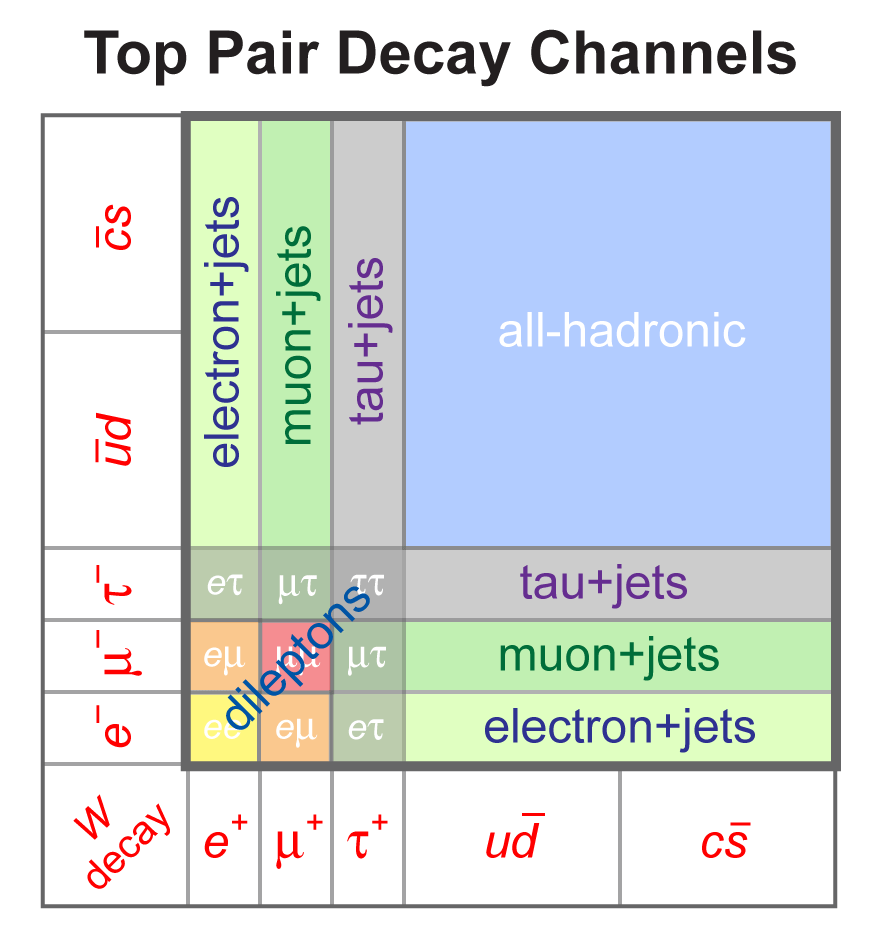
\includegraphics[width=0.49\textwidth]{01_Theory_SM/plots/top_pair_decay_channels.png}
\end{subfigure}
\begin{subfigure}
  \centering
  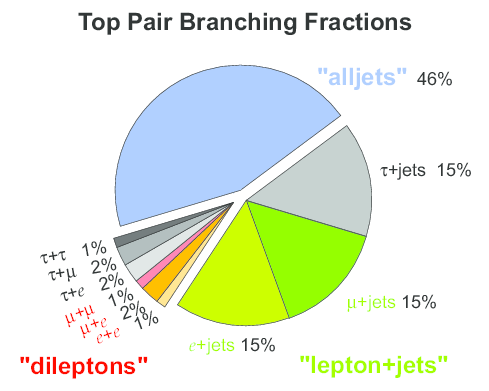
\includegraphics[width=0.49\textwidth]{01_Theory_SM/plots/top_pair_branching_frac.png}
\end{subfigure}
\caption{$t\bar{t}$ decay channels. On the right the branching ratio of different decay channels are shown. The diagrams are taken from \cite{UsefulDiagrams}.}
  \label{fig:tt_decay}
\end{figure}

\begin{itemize}
 \item \textit{Full hadronic channel}. Both $W$ bosons decay into quark-antiquark pairs -- $t\bar{t} \rightarrow (W^{+} \rightarrow q\bar{q}')b\:(W^{-} \rightarrow q''\bar{q}''')\bar{b}$.
 This decay channel has the largest branching ratio\footnote{The \textit{branching ratio} of a specific decay of a particular particle/system is the probability of this particle/system
 to decay via this decay mode.}. However, this state has a not very pure quality in the Large Hadron Collider environment, as a large number of quark and gluon jets is produced and similar
 final states are produced in many other non top production processes at the LHC.
 
 \item \textit{Semileptonic (lepton+jet) channel}. One $W$ boson decays hadronically, another one - into two leptons:  $t\bar{t} \rightarrow (W^{\pm} \rightarrow q\bar{q}')b \: (W^{\mp} \rightarrow l^{\mp}\nu)\bar{b}$.
 The high momentum lepton, which occurs in this process, is a signature that helps to identify the decay.
%  The semileptonic decay is an over-constrained system with 22 known components of four vector components of
%  jets and leptons and two $W$-mass constraints.
 
 \item \textit{Dileptonic channel}. Both $W$ bosons decay into leptons -- $t\bar{t} \rightarrow (W^{+} \rightarrow l^{+}\nu_{l^{-}})b \: (W^{-} \rightarrow l^{-}\bar{\nu}_{l^{-}})\bar{b}$.
 This decay channel has the smallest branching ratio, but the two high momentum leptons are a clear signature which helps to distinguish this final state from other processes
 occurring in the Large Hadron Collider collisions.
\end{itemize}

This analysis is based on the dileptonic channel. However, only the final states with one electron and one muon of opposite charge is considered. The ones with the decaying into
an $e\mu$ final state $\tau$ leptons are not taken into account as signal.

% \subsection{Studies of the $t\bar{t}$ Production}

% The studies of the $t\bar{t}$ production process provide a very important test of the Standard Model. 
% 
% In particular, the $t\bar{t}$ production in the $pp$ collisions at the LHC is dominated by gluon-gluon fusion (sec. \ref{ssec:tprod}, Fig.\ref{fig:LO_tt_prod}), which 
% is precisely measured in the QCD. Thus, the $t\bar{t}$ production cross section measurement can provide constraints for the PDF and the strong coupling constant $\alpha_s$.
% The total $t\bar{t}$ production cross section is accurately calculated up to NNLO, which means that the experimental measurement of this cross sections provide a 
% test of perturbative QCD.
% On the other hand, the deviation from the QCD predictions may point to some processes beyond the Standard Model. In addition, a measurement of the $t\bar{t}$ production 
% cross sections may deliver information about various top properties, e.g. mass or spin of the $t$-quark.

\chapter{Experimental Setup}
Every theory needs to have experimental proof to show it's compatibility. Particle physics is tested on
the colliders.
% \\
% Before the Large Hadron Collider era the Standard Model was experimentaly tested up to the scale of ~TeV.
% But there was a strong demand to raise the scale and implement the studies of electroweak symmetry breaking
% and Higgs mechanism.
% Physics beyond SM is also of interest on the scales above 1 TeV.
% The Large Hadron Collider\cite{LHCmachine} was providing the collisions with a centre-of-mass energy
% up to 8 TeV which is an eightfold increase of the scale compared to the previosly most powerful collider TEVATRON.
% \\


This chapter is devided into three parts.
The first part is denoted to the description of the Large Hadron Collider. The second part of the 
chapter is revealing the CMS detector construction and features in more detail as it was used to produce the final
results of this work. The third and the last part of this chapter is about the upgrade plans for the
CMS detector to operate with higher energies and luminosities.

\section{Large Hadron Collider}

The fastest protons in the world, ever controlled by human, are alive in Switzerland at CERN.
The Machine which can manage the operation of these protons is called Large Hadron Collider(LHC). 
The LHC is a ring-shape tunnel 26.7 km long  placed 45 - 170 m unground. 
Inside the tunnel there are two rings with vacuum tubes where proton(or lead nuclei) beams are circulating in different directions.
There are four locations where the rings are crossing and the protons can collide with each other. 
The designed center-of-mass energy for those collisions is $\sqrt{s}$ = 14 TeV, which means 7 TeV in one direction.


Not to get out of the ring 7 TeV protons are guided by 8 T superconducting magnets. 
For optimal usage of these magnets one needs to preaccelerate and preforme the proton banches.
For this porpose LHC is supported by preacceleration system shown at Fig. \ref{fig:AccelCERN}


The way of the protons literally starts from a bottel of hydrogen gas.
H2 atoms entering 

%[http://www.lhc-closer.es/1/3/10/0]

%To kep running LHC during the 2012 data taking periud was used only 1 cubic suntemiter of H2 gass.
\begin{figure}[t]
  \centering
  %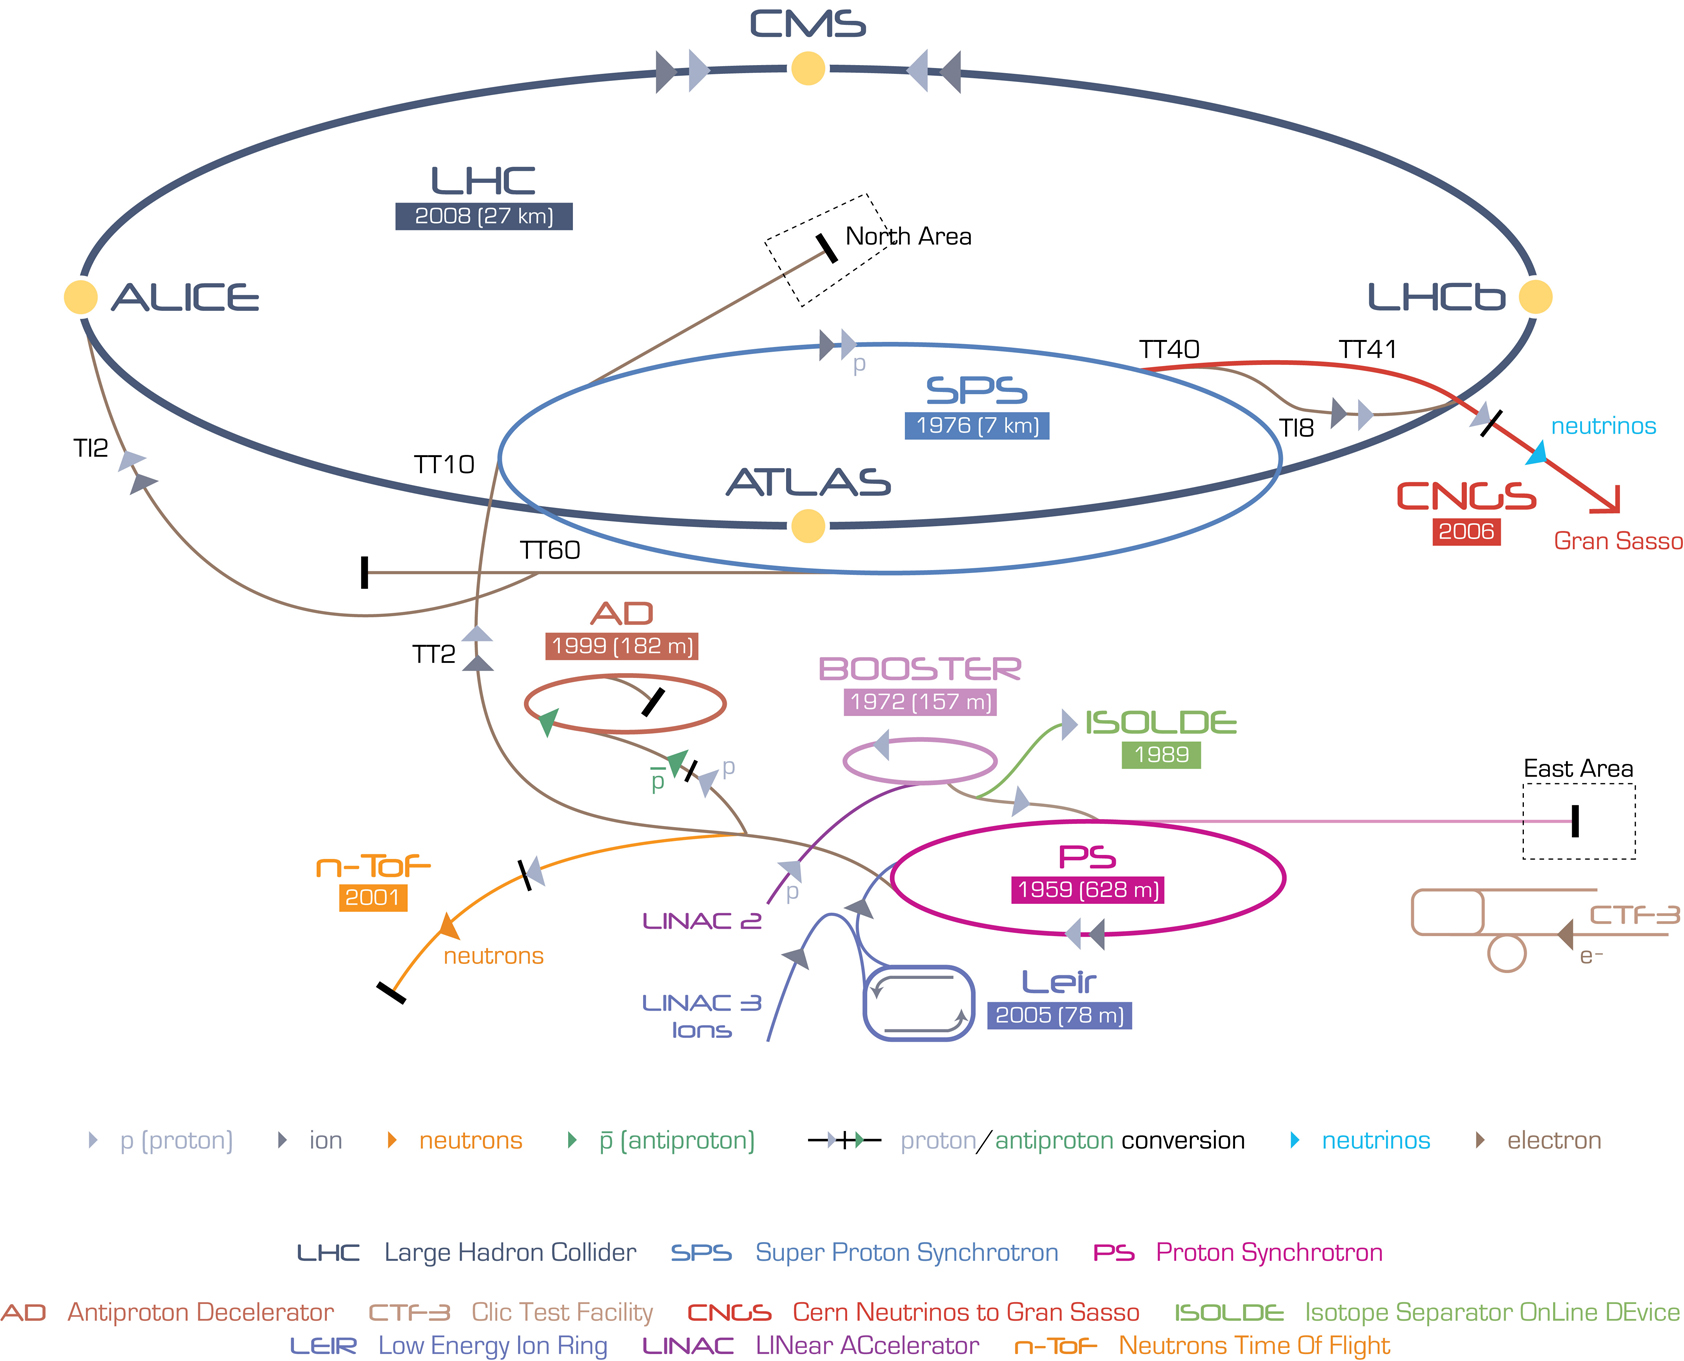
\includegraphics[width=0.6\textwidth]{02_experimental_setup/plots/Cern-Accelerator-Complex.png}
  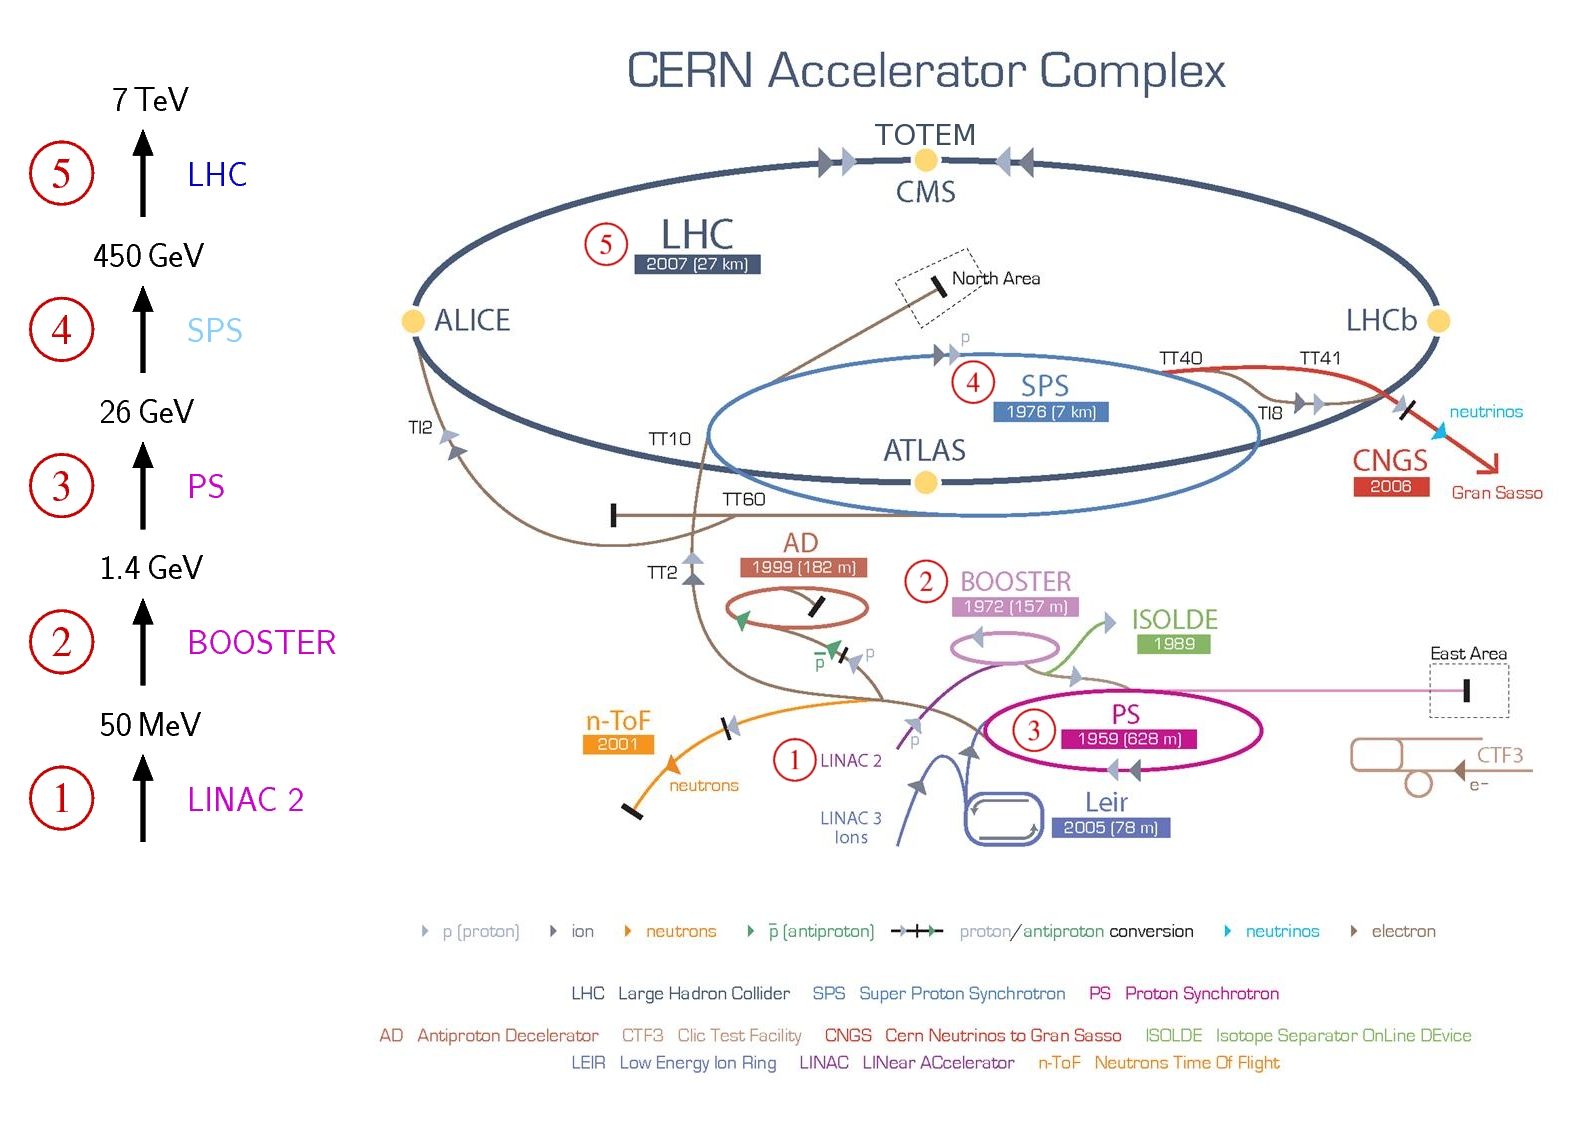
\includegraphics[width=0.6\textwidth]{02_experimental_setup/plots/Cern-Accelerator-Complex-2.png}
  \caption{The complex of accelerators at CERN with their length and particles being accelerated inside.}
  \label{fig:AccelCERN}
\end{figure}


% Each accelerator in the chain boosts the energy of the particles beams and injects them to the next machine in
% the preaccelerator chain. The LHC is the last accelerator in the sequence.
% \\
% \\
% The first accelerator on the way to the LHC is the Linac2. It injects protons or heavy ions to the Proton Synchrotron
% Booster (PSB). Then the particle beams arrive to Proton Synchrotron (PS) followe by Super Proton Synchrotron (SPS).
% \\
% \\
% And finaly the beams are transfered to the two pipes of the LHC. Beams inside one of the pipes circulate clockwise
% and in the other -- anticklockwise. 
% \\
% \\
% The whole preaccelerations takes four and a half minutes, while the particles in the LHC circulate 20 minutes
% to reach the final energy.
% \\
% \\
% ------The designed working centre-of-mass energy at the LHC is $\sqrt{s} = 14 TeV$, but from the safety
% point of view it first operated at the smaller energies -- $\sqrt{s} = 7 TeV$ and $\sqrt{s} = 8 TeV$ up to
% the end of 2011 and 2012 correspondingly.
% \\
% \\
% And after a long shutdown and a sequence of the upgrade workarounds the machine is ready for the operation
% with the centre-of-mass energies of $\sqrt{s} = 13 TeV$ and finally $\sqrt{s} = 14 TeV$. 
% \\
% \\
% ------Another parameter of the LHC which is very important for the experimental results is the \textit{luminosity}, $L$.
% \\
% \\
% It desribes the rate of events $\frac{dN}{dt}$, taking their cross section $\sigma$ into account:
% 
% \begin{equation}\label{eq:lumi}
%   L \sigma = \frac{dN}{dt}.
% \end{equation}
% 
% Equation\ref{eq:lumi} shows that the measurement of the cross section of any process needs the luminosity 
% value, which is an accelerator parameter and is given as\cite{CMStdr}:
% 
% \begin{equation}
%  L = \frac{\gamma f k_{B} N_{p}^2}{4 \pi \epsilon_{n} \beta} F,
% \end{equation}
% 
% where $\gamma$ is a relativistic gamma factor, $f$ is a revolution frequency, $k_{B}$ is a number of bunches,
% $N_{p}$ is a number of particles per bunch, $\epsilon_{n}$ is a normalized transverse emittance (designed value
% is 3.75$\mu m$), $\beta$ is the focus of the beam and $F$ is a reduction factor due to the crossing angle at the 
% interaction point.
% \\
% \\
% The designed luminosity is $L = 10^{34} cm^{-2}s^{-1}$ which leads to arround 1 billion proton-proton 
% interactions per second.
% \\
% \\
% ------There are other accelerator parameters which are relevant for the physics analysis. Some of them were
% mentioned above.
% \\
% \\
% Bunches of protons are formed in the PS with the time spacing of 25 $ns$. The number of proton bunches in the LHC is
% 2808. Each bunch has $11 $
% \\
% \\
% ------
% \\
% \\

The measurements of collision products are done with the complex particle detectors. There are four of them, 
\textit{ALICE}, \textit{LHCb}, \textit{ATLAS} and \textit{CMS}, on the LHC
ring, each located around the point where beams of particles of different directions are brought together.
These detectors have different construction thus having slightly different goals.

\begin{itemize}
 \item The ALICE (A Large Ion Collider Experiment)\cite{ALICEtdr} is designed to
 work with the heavy ion collisions. The goal of the ALICE experiment studies is
 the strongly interacting matter in extremely high density state called \textit{quark-gluon plasma}. This 
 state of matter provides a unique possibility to find a bare quark without a pair and also to study the early
 Universe which was so dense at the first moments after the Big Bang.
 \\
 The ALICE detector weights 10000 tonnes and is 26 m long, 16 m high and 16 m wide. It sits on the depth of
 56 m below the ground.
 
 \item The LHCb (Large Hadron Collider beaty)\cite{LHCb} is investigating the $CP$ violation and hevy flavour physics via
 the rare $B$ hadron decays. As the $b\bar{b}$ pairs are mostly produced in the forward and backward directions, 
 and their production cross section is very high there was no need to construct a big and expensive $4\pi$ detector 
 complex. For this reason the LHCb is a one side spectrometer corresponding to the forward beam direction.
 For a better detection of the $b$-decays the LHCb features a movable tracking system which can go very close
 to the beampipe.
 \\
 The LHCb detector weights 5600 tonnes and is 21 m long, 10 m high and 13 m wide. It sits on the depth of 100 m 
 below the ground.
 
 
 
\end{itemize}

% \section{The Compact Muon Solenoid}
% \subsection{Tracking Detector}
% \subsection{Electromagnetic Calorimeter}
% \subsection{Hadronic Calorimeter}
% \subsection{Muon Detector}
% \subsection{Trigger system}
% 
% \section{Upgrade for RunII}
% \subsection{CMS Pixel Tracker Upgrade}

\chapter{Upgrade of the Pixel Tracker}\label{chapt:pixel}

The CMS detector as described in chapter \ref{chap:exp_setup} was performing during the time period 
between 2010 and 2012. It provided a center-of-mass energy up to 8 TeV and the bunch spacing was 50 ns. 
However, the LHC program was planned for at least a decade longer and the plan includes several improvements.

After the shutdown for two years, from the end of 2012 until the beginning of 2015, the LHC 
center-of-mass energy was increased up to 13 TeV and will be further increased to the designed value
of 14 TeV. The next long shutdown is planned in 2018. Until that time it is planned that the peak
luminosity will reach $10^{34} \text{cm}^{-2} \text{s}^{-1}$ (comparing to the $7 \cdot 10^{33} \text{cm}^{-2}\text{s}^{-1}$
reached in 2012). The total integrated luminosity which is planned to achieve prior the second long shutdown
is 100 fb$^{-1}$ \cite{CMS:2012sda}. This LHC phase is called \textit{Phase 0}.

The plan after the second long shutdown (2018) is to increase the brightness of the bunches
in the accelerators. This is planned to be done with improving the injectors. In the period 
after a second long shut down and until 2022 (so-called \textit{Phase 1}) the LHC will reach
a peak luminosity of $2-3 \cdot 10^{34} \text{cm}^{-2} \text{s}^{-1}$ and deliver about 
300 fb$^{-1}$ of data \cite{Rocca:2014soa}. 

The third long shutdown in 2022-2023 will be used for the improvements of the LHC accelerating system by
exchanging the aged parts by the new and improved ones (focusing magnets, cryogenics system, etc.).
After these improvements, the LHC is expected to reach a peak luminosity of $2-3 \cdot 10^{34} \text{cm}^{-2} \text{s}^{-1}$.
The period of LHC operation after the third long shut down is called \textit{Phase 2} \cite{Rocca:2014soa}.

It is natural that the changes of the accelerator systems have to be reflected also in the detector construction.
If the collisions with higher energies and frequencies are provided by the accelerator machine, the detector might
be overloaded with information and some of its parts might be damaged by the higher radiation. That is why 
the CMS is also being upgraded simultaneously with the LHC.

The silicon pixel tracker (see the description in sec. \ref{sec:tracker}) is the innermost part of the CMS 
detector mounted around the beam pipe and being the closest detector to the collision point. That means that
it receives the highest irradiation dose and operates in a very dense particle environment. After the upgrade 
in 2015 the conditions for the pixel tracker will get even more severe. That is why it has to be significantly 
upgraded to perform with the sufficient precision. 

This chapter describes the studies performed in frames of the fourth layer barrel pixel detector upgrade for the
LHC Phase 1. It is mainly concentrated on the barrel pixel tracker, and specifically on the tests for the
planned fourth layer of the latter.

\section{Plan For the Upgrade of the Barrel Pixel Tracker}

This section will give a brief overview of the plan for the whole CMS silicon pixel upgrade in frames of so-called
Phase I upgrade. The purpose of this upgrade is to remake and update the present silicon pixel tracker to make it 
suitable for the high luminosity and energy runs which will start after the year 2016. The replacement of the silicon
pixel tracker is planned for the technical stop in 2016/2017. 

The main goal for the updated pixel detector is that it should function at higher luminosities with the same or even
better performance as the current pixel tracker on the lower luminosities \cite{CMS:2012sda}. For these needs new read-out chips
(ROCs) have to be designed such that the data losses are minimized. In addition, the readout system as well as all
the other detector components have to be radiation hard, as the expected doses which the detector has to meet (especially
the first layer, which is the closest to the beam pipe) are much increased.

It was also decided to increase the number of barrel layers of the pixel detector from 3 to 4 (see Fig. \ref{fig:tracker_4}).
They were designed as four concentric cylinders with a length of 548.8 mm and radii between 30 mm and 160 mm.
This improves the track identification, which is crucial in the environment with a twice higher pile-up, expected for the 
LHC run after 2017. In addition the innermost layer of the detector is moved closer to the collision point (by 10 mm), while
the layers 2 and 3 are almost unchanged in the position. The beam pipe
will also be made smaller to allow the closer approach to the interactions.

Each layer will constructed of various number of 22 mm wide facets, in total consisting of 1184 rectangular pixel modules. Each module
consists of 16 pixel chips. The total number of pixels will be increased from roughly 48 M to 79 M.

\begin{figure}[t]
 \centering
 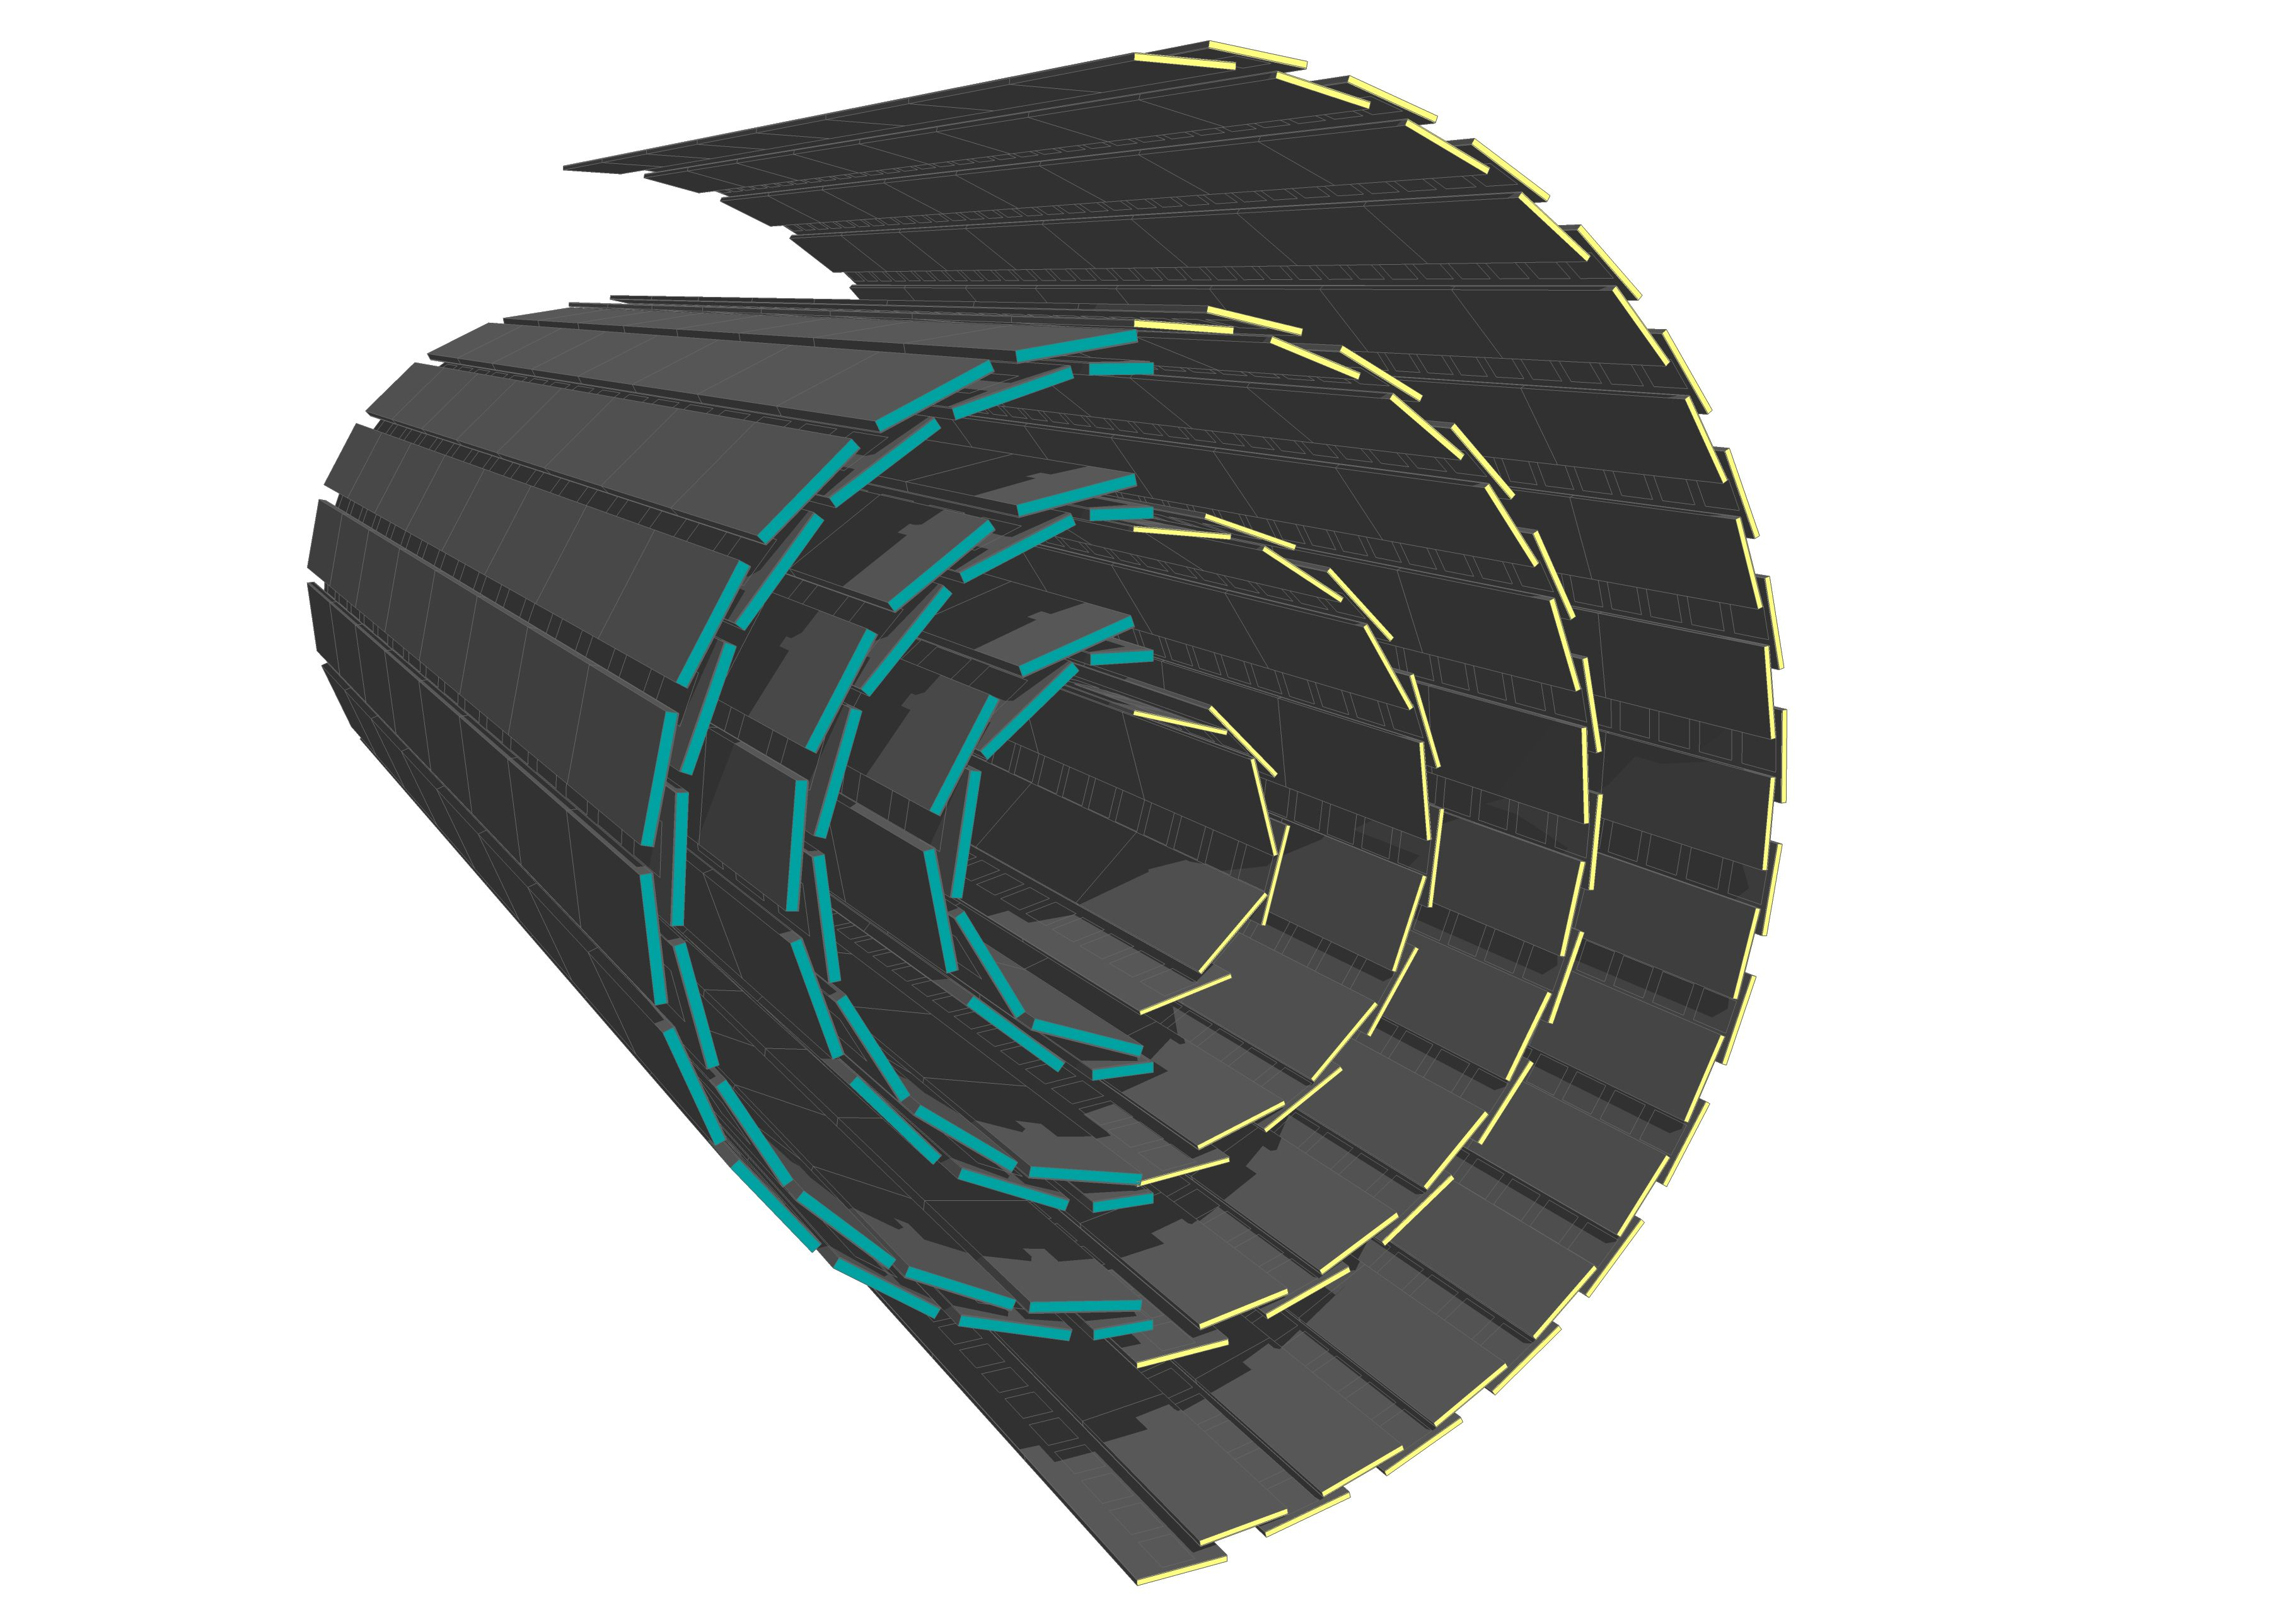
\includegraphics[width=1.0\textwidth]{021_pixel_upgrade/plots/pixel_phase1_4_layers.png}
 \caption{The model of the barrel pixel tracker before (on the left) and after the Phase 1 upgrade (on the right). Figure taken from
 \cite{CMS:2012sda}.}
 \label{fig:tracker_4}
\end{figure}

The addition of the fourth layer increases the amount of material which the particles have to go through. This is not
the desired feature for the innermost detectors. So the volume of the material, which the detector is made of, has to be decreased. 
First of all, the readout system itself is planned to be thinner (it is easy to see in the Fig. \ref{fig:tracker_4},
where the new pixel barrels are thinner). Secondly, the electronic boards will be moved out of the detector volume. 
Additionally, a new $CO_{2}$ cooling system \cite{CMS:2012sda} with a light-weight mechanical support will save material budget.

The improvements planned will lead to higher efficiencies, lower fake track rates (see sec. \ref{ssec:trkReco}), lower read-out dead time,
and extended lifetime of the detector. This results in a better identification of the particles for offline analysis and HLT.

The planned upgraded detector performance was simulated. It was compared to the performance of the non-upgraded tracker. This comparison
is shown in Fig. \ref{fig:sim_perform}. These simulations were performed on the simulated $t\bar{t}$ samples. The studies show overall higher 
efficiencies and lower fake rates for the upgrade detector for the higher puleup scenarios.

\begin{figure}[p]
 \centering
 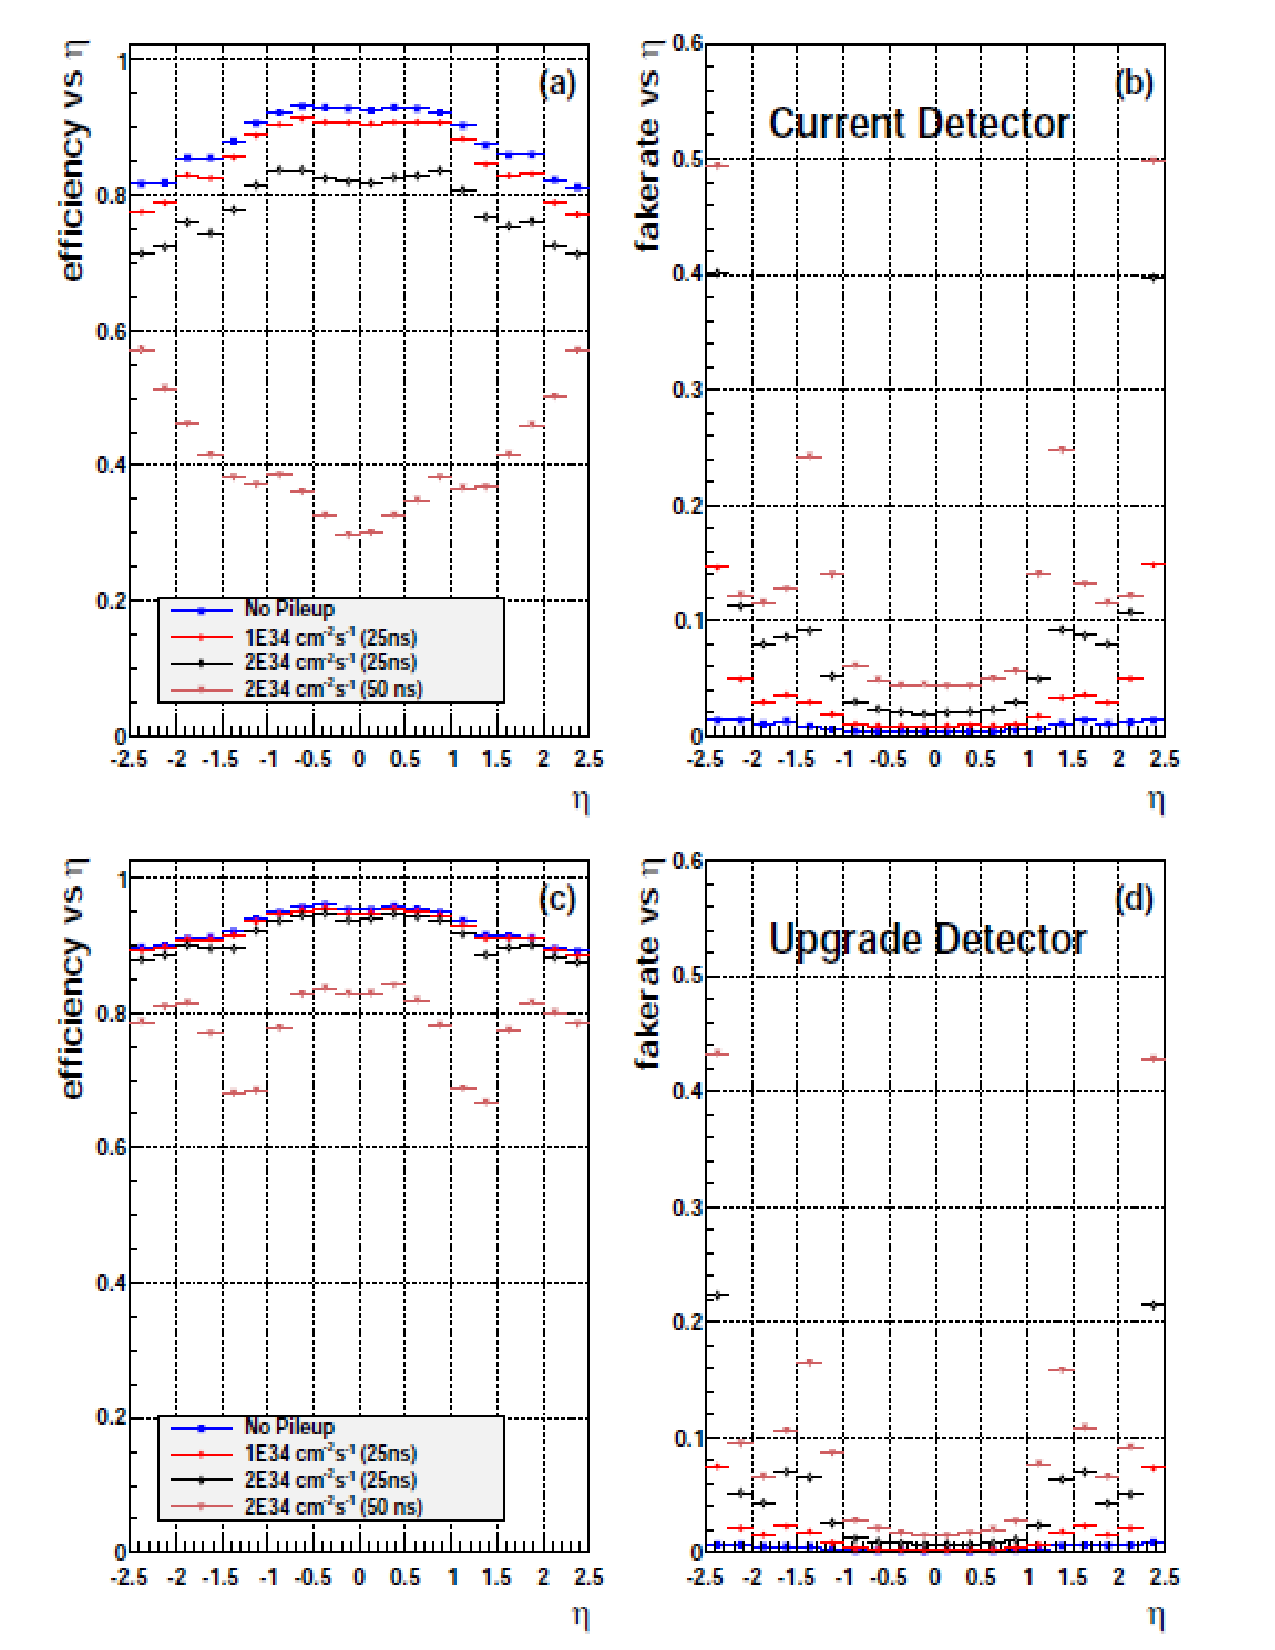
\includegraphics[width=0.8\textwidth]{021_pixel_upgrade/plots/sim_perform.pdf}
 \caption{Tracking efficiency (a,c) and fake rate (b,d) for the simulated $t\bar{t}$ sample as a function of track
          pseudorapidity $\eta$, for the current detector (a,b) and the upgrade pixel detector (c,d). Results are shown for
          zero pileup (blue squares), an average pileup of 25 (red dots), an average pileup of 50 (black
          diamonds), and an average pileup of 100 (brown triangles). The ROC data losses were simulated
          as expected at each given luminosity. The plot is taken from \cite{CMS:2012sda}.}
 \label{fig:sim_perform}
\end{figure}


\section{Studies of Irradiated Prototype Modules}

The expected performance of the barrel pixel tracker was confirmed in the simulated experiments. However, it is also crucial to test 
the performance of the device under real conditions. 

Prototype single chips were produced for the needs of such tests. These are chips of the design which was meant for the production
of the real detector facility, but supplemented with a separate readout system and board to enable an independent operation of such
a chip. 

In this work tests of the prototype chips for the fourth layer barrel pixel (BPIX) detector were performed. The layout of the prototype chip is shown 
in Fig. \ref{fig:prototype}. The chip is a 1/16 part of the modules from which the pixel detector will consist. 
One prototype chip contains 80 rows and 52 columns of pixels, each of the size $100\times150$ $\mu$m$^{2}$.
These pixels collect electrons from oxygenated high-resistivity $n$-type silicon sensors of 285 $\mu$m thickness with n+ implants. 

\begin{figure}[t]
 \centering
 \begin{subfigure}
  \centering
  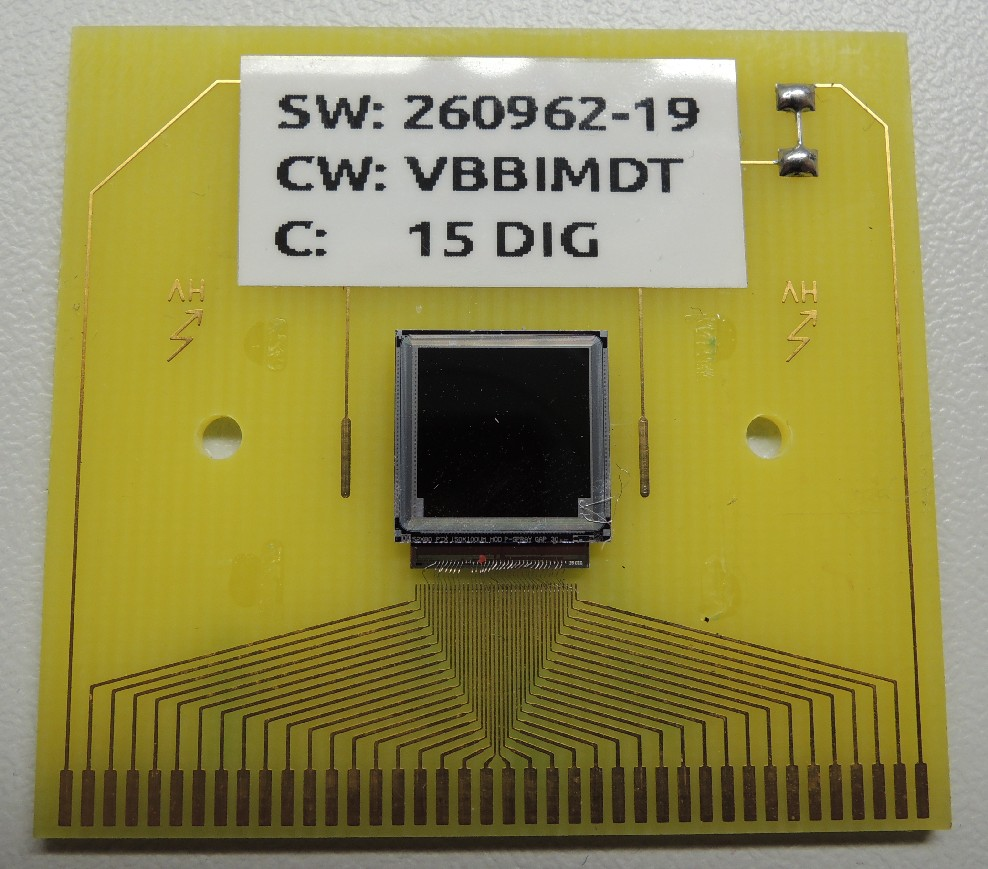
\includegraphics[width=0.4\textwidth]{021_pixel_upgrade/plots/prototype_chip_photo.png}
 \end{subfigure}
 \begin{subfigure}
  \centering
  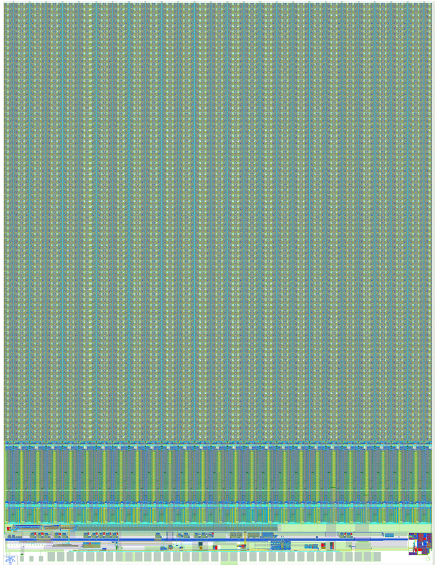
\includegraphics[width=0.4\textwidth]{021_pixel_upgrade/plots/prototype_chip.png}
 \end{subfigure}
 \caption{The photo of the prototype silicon pixel chip for the Phase I upgrade of the CMS BPIX, layer 4, mounted to the readout panel (on the left)
 and a magnified readout chip layout print (on the right).}
 \label{fig:prototype}
\end{figure}

Each pixel is bump-bonded to the ROC of the same height and width. The ROCs are fabricated in 250 nm CMOS (Complementary Metal-Oxide-Semiconductor)
employing the radiation hard design rules.
For the upgrade, the data buffer is increased to be able to work with higher occupancy connected with the higher data flow from the more frequent 
and dense LHC collisions. Furthermore the measured charges are digitalized and transmitted at 160 MHz. The effect of the internal cross talk is reduced
by design optimization and use of the 6 metal layers for the circuit, which allowed to operate at lower thresholds.

One of the important tests was to examine the chips with new design with respect to their radiation hardness. As discussed before the
pixel detector will receive the maximum dose of the radiation being the closest detector part to the collision point (see Fig. \ref{fig:irrad_dose}).
It is expected that the dose absorbed by the layer 1 of BPIX during the full lifetime of the detector will be 100 MRad, or 1 MGy. Layer 2 is 
expected to absorb 40 MRad (0.4 MGy), layer 3 -- 20 MRad (0.2 MGy) and layer 4 -- 13 MRad (0.13 MGy).

\begin{figure}[t]
 \centering
 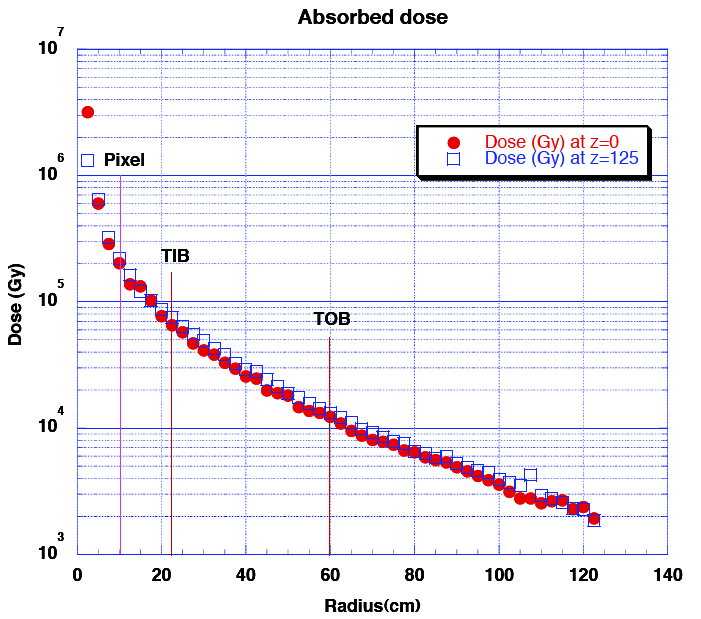
\includegraphics[width=0.8\textwidth]{021_pixel_upgrade/plots/irradiation_dose.png}
 \caption{The dose in Gy on to be absorbed by different tracker parts at different radial distance from the LHC $pp$ beam line for different
 $z$ coordinate values. The average position of the pixel detector is marked with a red vertical line. The location of different parts of the 
 silicon strip detector are also shown for comparison. The dose is defined for the expected full run time of the LHC until 2018, which 
 corresponds to the integrated luminosity of 500 fb$^{-1}$. The plot is taken from \cite{CMS:2012sda}.}
 \label{fig:irrad_dose}
\end{figure}

Here the studies of the properties of the irradiated prototype chips for layer 4 of BPIX will be presented. For this purpose the prototype
chips were irradiated at the CERN PS \cite{CERNTB} with the 23 GeV protons up to fluences of 3.8 $\cdot$ 10$^{14}$ $p/cm^{2}$ which corresponds to 
the expected lifetime dose of the layer 4 of the BPIX (approximately 16 MRad). 

The prototype chips were irradiated such that the silicon sensor side was facing the beam. The readout chips on the back side received a dose
up to 130 kGy. The tests  in the laboratory at DESY \cite{DESYWeb} showed the full functionality of the irradiated ROCs.

\subsection{DESY Beam Test}

To test the functionality of the prototype silicon pixel chip, one needs to deliver some particles with relatively high energy and let
the chip register them. For this purpose so called ``beam tests'' are performed. For the studies described in this thesis, the DESY beam test
facility was exploited.

The DESY beam test facility makes use of the electron-positron synchrotron DESY II \cite{Hemmie:1982xq, DESYIIWeb}, which provides electron
and positron beams with up to 1000 particles per cm$^{2}$ at energies of up to 6 GeV. However, these are not the particles which are directed
to the beam test areas. The circulating DESY II beam hits the 25$\mu$m thick carbon fiber and emits bremsstrahlung. The resulting photons are afterwards 
converted to electron-positron pairs on the converter, which is actually a copper plane. The resulting beam is passed to a dipole magnet for
separating the particles with the required momentum. Afterwards the beam is collimated and brought to the area where it can be exploited for the
experimental needs. The scheme of the facility which delivers the beam for the tests is shown in Fig. \ref{fig:desy_tb}.

\begin{figure}[t]
 \centering
 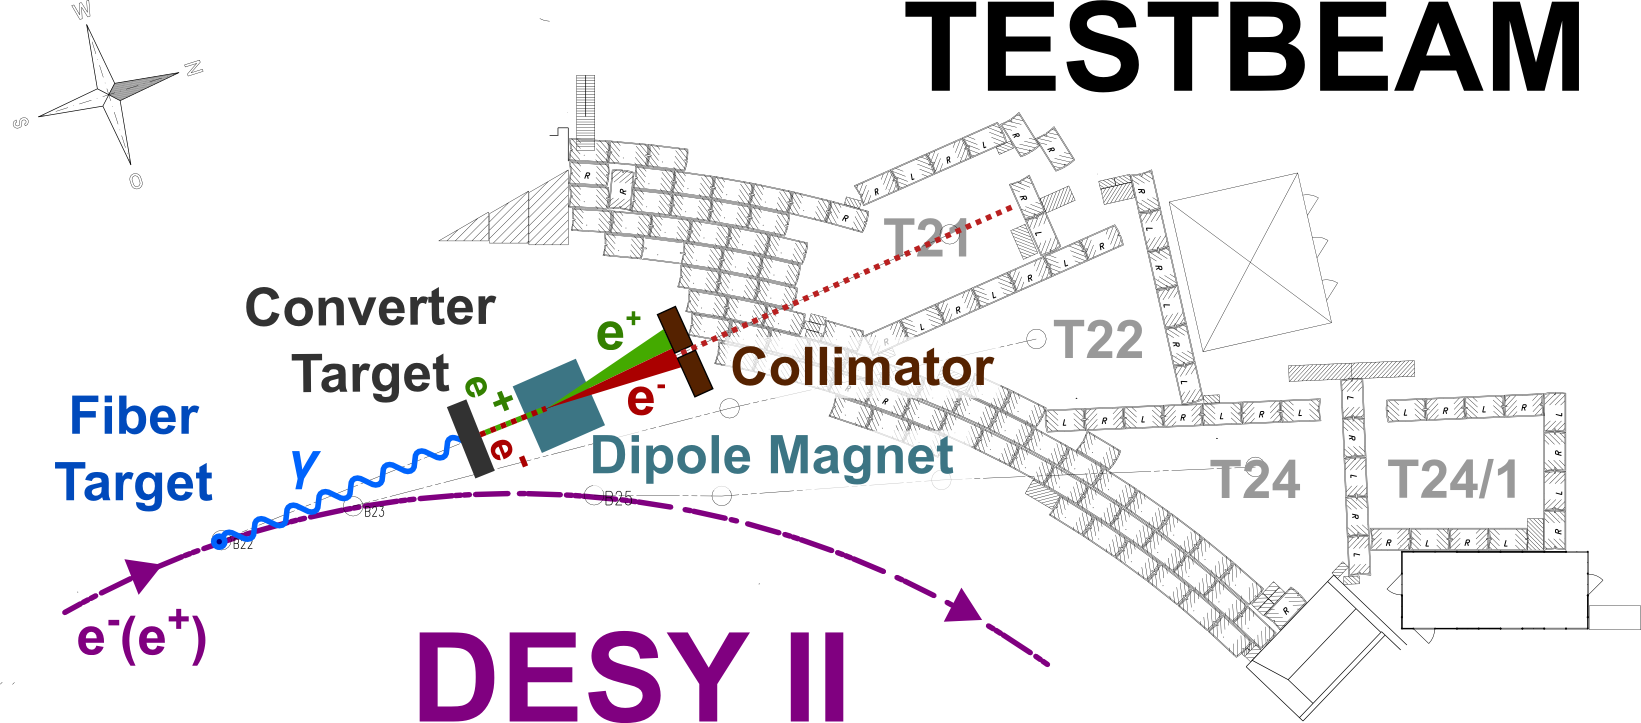
\includegraphics[width=1.0\textwidth]{021_pixel_upgrade/plots/desy_tb-sketch.png}
 \caption{Schematic layout of the test beam facility at DESY. The plot is taken from \cite{DESYTBArea}.}
 \label{fig:desy_tb}
\end{figure}

\subsection{EUDET Telescope and Experimental Setup} 

The beam test line where the tests described in this thesis were performed is equipped with a telescope of the EUDET/AIDA-family \cite{EUDET},
which is shown in Fig. \ref{fig:EUDET_tel}. It consists of two arms each equipped with three sensors kept at a stable temperature by a cooling
system. Each sensor plate can be moved along the beam axis to meet some particular experimental requirements.

\begin{figure}[t]
 \centering
 \includegraphics[width=1.0\textwidth]{021_pixel_upgrade/plots/Fig1.pdf}
 \caption{Photo of the EUDET telescope present at the beam test line 21 at DESY. The device under test is installed in between the two
 groups consisting of three telescope plates each. The electron/positron beam impinges perpendicularly onto the EUDET telescope planes 
 coming in from the right side of this photo.}
 \label{fig:EUDET_tel}
\end{figure}

The telescope serves as a device which measures the particle path with a very good precision so that it is assumed to be known.
The EUDET telescope is equipped with silicon pixels. The telescope sensors have a point precision of 3.4 $\mu$m and they
are made with a minimum of material (their thickness is only 50 $\mu$m), so that the precision doesn't drop even on the lowest 
energy border of the test beam ($\sim$ 1 GeV), when the contribution of the interaction of the particles with matter (multiple
scattering) becomes sizable. The installed Mimosa (Minimum Ionizing MOS Active Pixel Sensor) sensors (with a size of 
$21 \times 11$ mm$^{2}$ with squared pixels with s size of 18.4 $\mu$m) developed for the EUDET telescope make use of the MAPS 
(Monolitic Active Pixel Sensors) technology \cite{2001NIMPA.458..677T, Fischer:2002bv}.

The prototype silicon pixel chip for the BPIX upgrade was placed in between two arms of the telescope. In the beam test 
campaign the tested device (in case of these studies it's the prototype chip) is called a Device-Under-Test (DUT). The DUT
and it's board are placed in a special frame which allows tilting and turning (see Fig. \ref{fig:prototype_board}). 
This enables studies of the detector behavior with inclined particle tracks producing multi-pixel clusters. 

\begin{figure}[t]
 \centering
 \includegraphics[width=1.0\textwidth]{021_pixel_upgrade/plots/prototype_board.png}
 \caption{Photo of the DUT (prototype silicon pixel chip for the BPIX 4$^{th}$ layer upgrade) and it's board in the metal frame
 mounted between two arms of the EUDET telescope at the DESY beam test area.}
 \label{fig:prototype_board}
\end{figure}

There is a second CMS prototype chip placed downstream at the end of the beam telescope. It had to serve as a reference for the
measurement of the DUT efficiency, as it has the same time of the working cycle as the DUT (25 ns). The Mimosa has a much longer
cycle (115 $\mu$s) and it can't be used as a reference for the DUT.

On the front before and in right after the telescope two crossed scintillators are located. They serve as a trigger. 
If their signals coincide, the particle has passed all the way through the telescope.
The typical duration of one run when the telescope, DUT and reference chip were registering the test beam particles, was from 10
to 30 minutes having several hundred thousand trigger signals.

\subsection{Data Taking}

The data from the telescope was passed to the computer through network cables (see Fig. \ref{fig:EUDET_tel}) and from
the CMS prototype chips -- through USB cables (see Fig. \ref{fig:prototype_board}). These are the signals which inform
about the particles hitt the detector plane.  Afterwards the received data had to be preanalysed. 

To gain accurate knowledge of the geometry of the setup, alignment procedure was done with the Millipede algorithm 
\cite{1748-0221-3-09-P09002}.

The neighboring fired pixels on the pixel detector are grouped into clusters and the centers of the clusters are the hits.
The tracks were reconstructed from the hits using the general broken lines algorithm \cite{Blobel:2006yi}. It takes into
account the multiple scattering in the detector. 

To define the telescope resolution, first the particle track was reconstructed using the hits in the first and third telescope planes.
Then the second plane was used to determine the difference between the reconstructed particle track position and the actual hit in the 
second telescope plane.

This basic information from the telescope and from the prototype chips is used for the further analysis.

\subsection{Analyzing the Prototype Chip Properties}

Several crucial properties which are important for the future BPIX detector operation were measured during the DESY test beam 
campaign.

\subsubsection{Charge Collection}

The external bias voltage is needed to collect all the charge which was released due to the particle crossing the sensitive silicon
pixel of the detector. If the bias voltage is not high enough, not all the charge is collected and the particle energy may be defined
incorrectly. The voltage at which the full charge starts to be collected is called \textit{depletion voltage}. The bias voltage is
applied on the $p$-implant side. A schematic path of the ionizing particle through the silicon sensor and of the resulting charge 
collection is shown in \ref{fig:depl_volt}.

\begin{figure}[h]
 \centering
 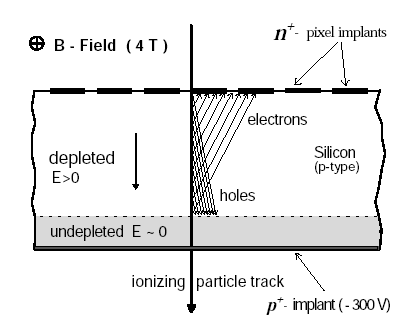
\includegraphics[width=0.6\textwidth]{021_pixel_upgrade/plots/depletion_voltage.png}
 \caption{The sketch of the charge collection from the ionizing particle crossing the silicon sensor. The figure is taken from \cite{}.}
 \label{fig:depl_volt}
\end{figure}

After the irradiation the damages in the silicon material are introduced. These damages may trap the ionized charge  which is traveling 
through the silicon to the place where it is read off. That is why a higher voltage is needed so that the particles overcome the traps.
However, there is a practical power dissipation related with the ohmic heating and on the bias voltage supply. If the depletion voltage
is higher than the voltage allowed by these limitations, the full depletion conditions for the sensors can never be reached. That is why 
it is necessary to test if the full depletion region can be reached and if so, then at which bias voltage.

To study this problem, the external bias voltage was varied from the very low values up to few hundred volts. The collected charge was
measured for each value of supplied bias voltage.

Fig. \ref{fig:depletion_voltage} shows the collected pixel cluster charge normalized to the maximum charge collected and tracking efficiency,
which was defined as the number of tracks which were registered in telescope, reference and DUT chips over the number
of tracks registered in telescope and reference chip.
These quantities are shown for two chips which were irradiated with doses of $0.9 \cdot 10^{14}$ p/cm$^2$ and $3.8 \cdot 10^{14}$ p/cm$^2$. 

\begin{figure}[t]
\centering
\begin{subfigure}
  \centering
  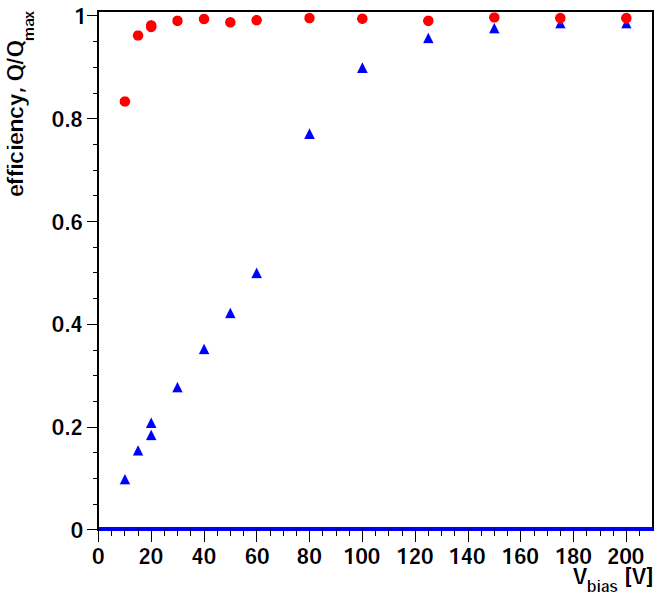
\includegraphics[width=0.42\textwidth]{021_pixel_upgrade/plots/voltage_scan_low_irrad.png}
\end{subfigure}
\begin{subfigure}
  \centering
  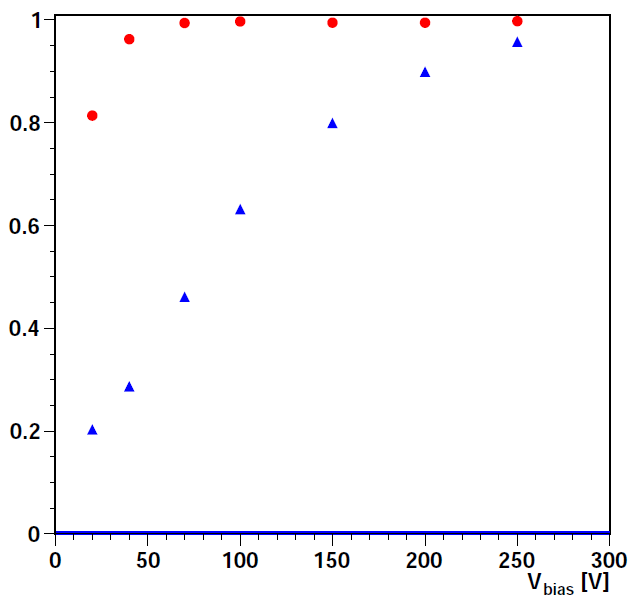
\includegraphics[width=0.4\textwidth]{021_pixel_upgrade/plots/voltage_scan_high_irrad.png}
\end{subfigure}
\caption{Charge collection efficiency, normalized to the maximum cluster charge (triangles) and tracking efficiency (circles) of the prototype silicon sensor
         for the CMS pixel tracker irradiated with $0.9 \cdot 10^{14}$ p/cm$^2$ (left) and $3.8 \cdot 10^{14}$ p/cm$^2$ (right) as function of the applied bias voltage.}
\label{fig:depletion_voltage}
\end{figure}

For the prototype chip which was irradiated with $0.9 \cdot 10^{14}$ p/cm$^2$, the collected charge drops quickly for bias voltages below -110 V. 
Only about one third of the charge is collected with a bias voltage lower than -30 V. However, the tracking efficiency still remains higher
than 90\%. This means, that the detector is fully efficient in terms of tracking with only one third of the charge collected.

For the chip with higher dose of $3.8 \cdot 10^{14}$ p/cm$^2$ full depletion is reached only with -250 V. The full tracking efficiency
is reached at -70 V, where around half of the charge was collected.

Additionally, the absolute pixel cluster charge distribution for the chip irradiated with a dose of $3.8 \cdot 10^{14}$ p/cm$^2$ was measured
with the -250 V bias voltage supplied (see Fig. \ref{fig:Landau}). It has an expected Landau shape, peaking at 18 ke. Before the irradiation a 
similar test was performed for this chip and Landau peak was at 22 ke then. This means that there is a charge loss due to trapping in the silicon
bulk after the irradiation.

\begin{figure}[t]
 \centering
 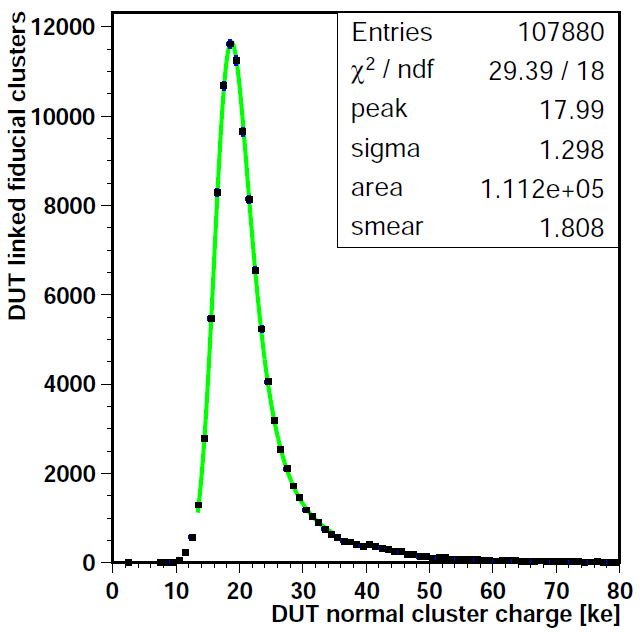
\includegraphics[width=0.6\textwidth]{021_pixel_upgrade/plots/Landau.png}
 \caption{Cluster charge distribution measured in the electron beam for a 285 $\mu$m thick pixel sensor irradiated with $3.8 \cdot 10^{14}$ p/cm$^2$ 
 at a bias voltage of -250 V (plateau region).}
 \label{fig:Landau}
\end{figure}

\subsubsection{Position Resolution}

The accuracy of the measurement of the position where the particle hit the silicon detector is primarily limited by the size of the silicon pixels.
However there is the way to improve the resolution using the charge sharing technique. If the charge from one particle will be collected in more
than one pixel, the position of the particle will be defined as the weighted average position of these pixels (the weighting is done corresponding 
to the amount of charge collected by each pixel). The charge sharing may happen either due to the inclined particle tracks with respect to the 
silicon sensor plane or because of the Lorentz drift in the magnetic field.

The particles from the DESY test beam were flying only in one direction. For the resolution improvement, the silicon chips were tilted by a certain 
angle with respect to the particle path to make the particles cross more than one pixel. This aims at obtaining an optimal charge sharing.

As discussed before, the irradiation introduces defects in the silicon which trap the charge carriers. This may influence the charge sharing
and thus the position resolution of the detector. It is also necessary to have the full charge collection to correctly measure the particle position.
Thus, the optimal bias voltage has to be delivered.

The resolution at the beam test was defined as the difference between the position of the particle hit defined by the DUT chip and the position of the
track defined in the telescope and extrapolated to the DUT. The telescope resolution (around 4.3 $\mu$m at 5 GeV beam energy and 150 mm spacing between
the telescope plane) is being quadratically subtracted.

To define the optimal tilt angle in the direction of the pixel rows of prototype chip, the DUT was tilted several times at different angles and the 
pixel row resolution\footnote{The \textit{row resolution} of the silicon pixel chip is the resolution of the coordinate in the pixel row direction. This
is the direction which an object would have if it would move from one row to the other staying inside one column.} was measured. Fig. \ref{fig:tilt_scan} 
shows the result of these studies for the prototype chip irradiated with a dose of $3.8 \cdot 10^{14}$ p/cm$^2$. As expected, first the resolution is 
getting better with increasing the tilt angle because the particle starts to pass through multiple pixels on it's way and the charge is shared between 
those pixels. After a certain optimal tilt angle, however, the resolution starts to get worse again. This is explained with a fact that the particle 
ionizes too many pixels initiating a very low charge in some of them. This charge doesn't overcome the threshold\footnote{A threshold on the charge 
collected is set on every pixel to avoid noise collection} level of a pixel and is lost. The plot shows that the minimum resolution is reached at 
the angle of around 20$^{o}$. Geometrically, the optimal charge sharing is expected at 19.3$^{o}$ tilt angle for 100 $\mu$m pixels and 285 $\mu$m 
sensor thickness. The higher angle which is practically measured may be explained by the trapping of deep charges. This means that the charges 
created in a silicon sensor by an ionizing particle trap on the defects starting from some depth of the sensor. Effectively it results in the
reduction of the sensitive thickness of the sensor, thus the tilt angle for an optimal charge sharing increases.

\begin{figure}[t]
 \centering
 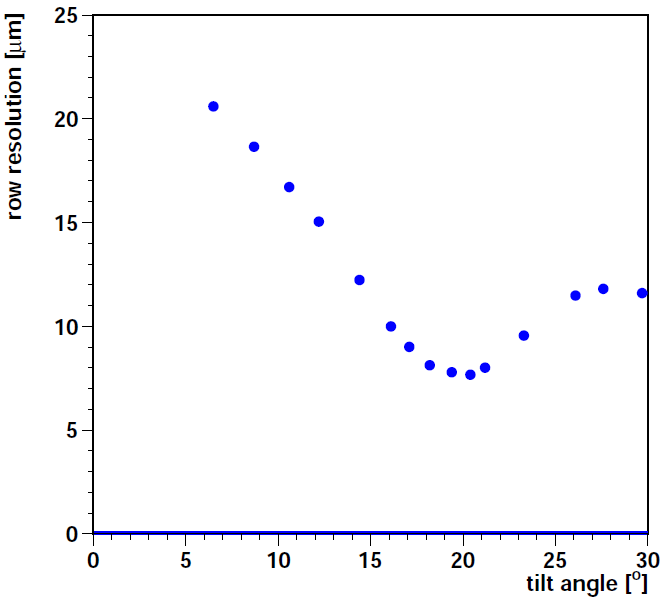
\includegraphics[width=0.55\textwidth]{021_pixel_upgrade/plots/tilt_scan.png}
 \caption{Resolution as a function of the tilt angle for a prototype silicon pixel module irradiated with $3.8 \cdot 10^{14}$ p/cm$^2$. The bias voltage  
 was set to -200 V and the threshold to 1.8 ke.}
 \label{fig:tilt_scan}
\end{figure}

For each point in Fig. \ref{fig:tilt_scan} the resolution in pixel row direction was determined as illustrated in Fig. \ref{fig:resol} using the 
width of the fitted gaussian. The plot shown is derived with the DUT tilted at 19$^{o}$.

\begin{figure}[t]
 \centering
 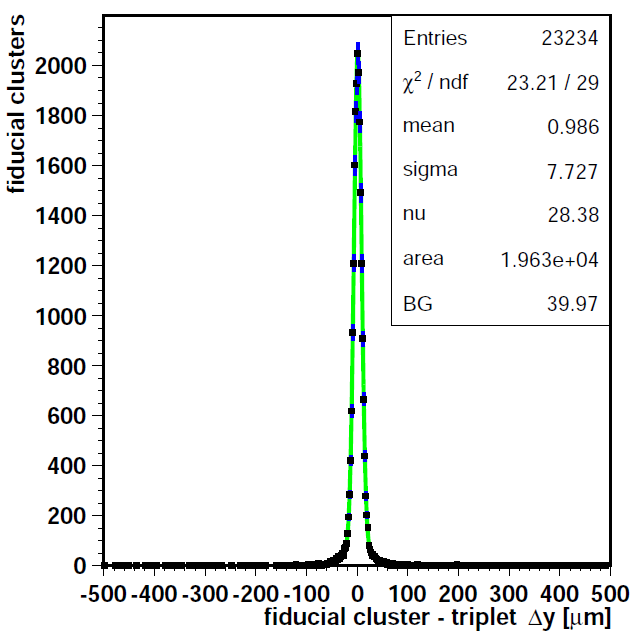
\includegraphics[width=0.6\textwidth]{021_pixel_upgrade/plots/resol_dist.png}
 \caption{Residual between DUT cluster position and telescope track in the direction of the 100 $\mu$m pixel size at a bias voltage of -320 V. The sensor 
 was tilted by an angle of 19$^{o}$ to the beam direction. The charge threshold was set to 1.8 ke. The fluence is $3.8 \cdot 10^{14}$ p/cm$^2$.}
 \label{fig:resol}
\end{figure}

The position resolution in the row direction was also measured for different bias voltages supplied. The result is presented in Fig. \ref{fig:bias_res}.
It shows that reducing the bias voltage below 150 V leads to a resolution degradation.

\begin{figure}[t]
 \centering
 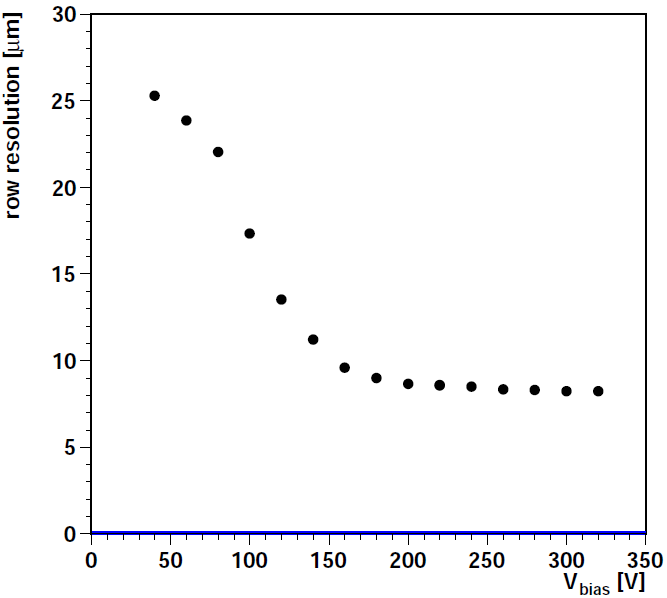
\includegraphics[width=0.55\textwidth]{021_pixel_upgrade/plots/bias_resol.png}
 \caption{Resolution as a function of the applied bias voltage without subtracting the telescope contribution, for a prototype silicon pixel module 
 irradiated with $3.8 \cdot 10^{14}$ p/cm$^2$.}
 \label{fig:bias_res}
\end{figure}

\subsection{Summary}

The prototype chips for the layer 4 of silicon pixel tracker for the CMS Phase 1 upgrade were operating after absorbing doses in order of and 
much higher than expected to be absorbed during the detector operation time. The damage effects caused by irradiation are observed. However,
the chips are fully operable and produce reasonable results. The resolution only slightly degrades -- the irradiated prototype has the resolution
of 6.4 $\mu$m in row direction, while before the irradiation this value was 5.5 $\mu$m. The full depletion after is reached at 150 V after the
irradiation.

In summary the tests of the prototype chips indicate that these types of chips meet the demands for operation after Phase I upgrade.

\chapter{Monte Carlo Simulation}

\section{Different Monte Carlo Generators and Models}
\subsection{Hard Scattering}
\subsection{Parton Showering}
\subsection{Hadronization Models}
\subsection{Simulated Samples}

\section{Detector simulation}

\chapter{Event Reconstruction}\label{chapt:event_selection}
 
The next step after gathering the available information from the detector machine (doesn't matter if it is a real or simulated facility)
is to interpret outcoming signals correctly. The task is to say which objects were present in the detecting apparatus using the hits
in the tracker, energy deposits in the calorimeter and signals from the muon system. Assigning this information to some concrete particle 
or object is a reconstruction procedure.

Different algorithms and methods are used to reconstruct different objects and some of them (relevant for this analysis -- leptons, jets and missing transverse
energy, responsible for neutrinos) are discussed in this
chapter. In general, for this analysis each object of the $t\bar{t}$ dileptonic final state was reconstructed using the information from many
CMS sub-detectors.


% 
% %%%%%%%%%%%%%%%%%%%%%%%%%%%%%%%%%%%%%%%%%%%%%%%
% \section{Particle Flow Concept}\label{sec:PF}
% 
% All the objects in $t\bar{t}$ dileptonic final state were reconstructed making use of \textit{Particle Flow} (PF)
% algorithm \cite{Beaudette:2014cea}. In other words each particle or jet is identified exploiting the information from all parts
% of the detector instead of using only one dedicated detector sector. The algorithm relies on an efficient track reconstruction,
% clustering algorithm in wich is able to distinguish overlapping showers and on the efficient linking procedure to connect 
% the signals from different sub-detectors.
% 
% A simplistic description of the reconstruction with the PF algorithm can be given as follows \cite{Beaudette:2014cea}.
% 
% \begin{itemize}
%  \item [--] Muons are identified beforehand to exclude overlapping with the charged hadrons. Their tracks are extrapolated
%  from tracker to calorimeter clusters and to the muon systems. An example of muon reconstruction using particle flow algorithm is 
%  shown on the figure \ref{fig:PFmuons}. The clusters in calorimeter and tracks in the tracker which the muons are assigned to
%  do not enter the further objects identification process.
%  %
%  \item [--] Charged hadrons are reconstructed from the tracks which after the extrapolation to the HCAL region fall within the boundaries
%  of one or more calorimeter clusters. Analogically to the tracks used for muon identification, tracks associated to the charged 
%  hadrons do not enter any further particle reconstruction.
%  %
%  \item [--] Electrons have to be reconstructed taking into account not only the tracks and ECAL deposits matching to them, but also
%  adding the photons from the frequent Bremsstrahlung.
%  %
%  \item [--] The remaining ECAL clusters are assigned to photons, and the one from HCAL - to the neutral hadrons
% \end{itemize}
% 
% \begin{figure}[t]
%   \centering
%   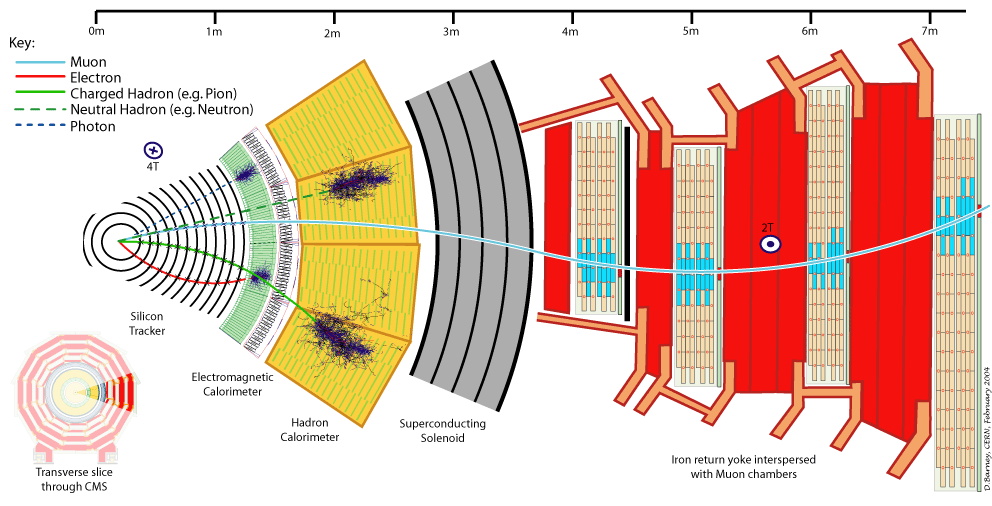
\includegraphics[width=1.0\textwidth]{04_event_reconstruction/plots/CMS_Slice.png}
%   \caption{Track reconstruction using different sub-detector information in combination in Particle Flow algorithm. An actual
%   muon track is shown with a curved blue line, an electron track is red and a charged hadron is solid green.}
%   \label{fig:PFmuons}
% \end{figure}
% 
% The resulting list of particles is used for further jet and missing transverse energy ($E_{T}^{miss}$) construction. 
% 
% The performance of the algorithm was studied with the simulated events \cite{CMS-PAS-PFT-09-001}. Particularly the jet energy
% resolution gain reaches factor 3 for a low transverse momentum region. Furthermore, the angular resolution is improved by factor 2-3.
% 
% A more detailed description of each object reconstruction relevant for this analysis is given in the following sections of this chapter.
% A complete overview of the PF algorithm can be found in \cite{CMS-PAS-PFT-09-001}. 
% 
% 
% %%%%%%%%%%%%%%%%%%%%%%%%%%%%%%%%%%%%%%%%%%%%%%%
% \section{Lepton reconstruction and selection}
% 
% The presence of two leptons, electrons or muons, is required for this analysis. Their reconstruction
% differs a lot due to a huge mass distinction. Thus, the reconstruction of leptons and muons is discussed separately.
% 
% \subsection{Muons reconstruction}
% 
% As it was discussed in section \ref{sec:CMS}, the CMS experiment has a well established setup for the muon reconstruction.
% Muons are the only particles expected to appear in the muon sub-detector system, thus their identification is unambiguous.
% Three techniques of muon reconstruction were implemented:
% 
% \begin{itemize}
%  \item [--] \textit{Standalone}: muons are reconstructed using the information from the muon system only. As 
%  this part of the detector provides a tracking information, a complete set of physical properties needed for the further
%  analysis is recorded.
%  
%  \item [--] \textit{Tracker}: the tracks, reconstructed in the tracking detector only, are assigned as muons in case they 
%  match at least one hit in the muon sub-detector. 
%  
%  \item [--] \textit{Global}: the muons are reconstructed using 
%  the combined fit of tracks from the muon system and from the inner tracker.
% \end{itemize}
% 
% Only the global or tracker muons were used for this analysis. It is more efficient to use the tracker algorithm to reconstruct
% low-momentum muons, but it suffers a lot from the presence of a large number of other particles. The global muons with small momenta
% are dominantly using the tracking detector information for the reconstruction, while starting from $p_{T} \sim \textrm{200 GeV}$
% the muon system data plays a significant role.
% 
% \subsection{Electrons reconstruction}\label{ssec:ElRec}
% 
% To reconstruct the electrons a combined information from the tracking detector and ECAL was used \cite{CMS-PAS-EGM-10-004}. The energy
% deposits in the ECAL are grouped into superclusters\footnote{A \textit{supercluster} is  a group of one or more associated clusters 
% of energy deposits in the ECAL. It is constructed taking into account its characteristic narrow width in the pseudorapidity $\eta$
% and its characteristic spread in $\phi$ due to the bending in the magnetic field of electrons radiating in the tracker material.} 
% with transverse energy $E_{T} > \textrm{4 GeV}$ and fitted to the tracks in the tracking detector \cite{GSF_Electron_Reconstruction_CMS}.
% 
% For a better quality of the tracks a restriction on the impact parameter\footnote{An \textit{impact parameter} $d_{xy}$ of the track is a minimum
% distance of the track to the primary vertex in the transverse $x-y$ plane.} $|d_{xy}| < 0.4 mm$ is applied. A maximum one hit in the inner tracker
% which is positioned close to the track, but not reconstructed, is allowed for the electron candidate.
% 
% On top of the mentioned conditions, a multivariate analysis (MVA) is performed to reduce the number of misidentified electrons.
% 
% \subsection{Lepton selection and isolation}
% 
% Only the events which contain at least two leptons (electrons or muons) with a minimum transverse momentum $p_{T}$ of 20 GeV reconstructed
% in central detector part $|\eta| \leq 2.4$ are accepted for the further analysis.
% 
% To distinguish leptons from hard processes (like a $W^{\pm}$ decay), or \textit{prompt leptons}, from the misidentified charged hadrons 
% and leptons from the jets, an \textit{isolation} criterion is required. The former usually don't overlap with jets, while the latter should
% fly in the same direction and be located in a close vicinity of a jet. This distinction is a basis for the isolation. An energy in a cone 
% around a lepton (not counting the lepton energy itself) is calculated. That is the definition of a combined isolation:
% 
% \begin{equation}
%  I_{comb} = I_{tracker} + I_{ECAL} + I_{HCAL} = \sum E_{photons} + \sum E_{hadrons}
% \end{equation}
% 
% The combined isolation $I_{comb}$ divided by the lepton transverse momentum $p_{T}(l)$ is the relative isolation used as a discriminant value:
% 
% \begin{equation}
%  I_{rel} = \frac{I_{comb}}{p_{T}(l)}
% \end{equation}
% 
% Leptons with the $I_{rel} \leq 0.15$ in the cone $\Delta R = \sqrt{\Delta\eta^{2} + \Delta\phi^{2}} = 0.3$ are selected.
% 
% \subsection{Lepton pair selection}
% 
% The $t\bar{t}$ decay final state has two oppositely charged leptons, while the selected events may contain three or more leptons.
% Out of all the leptons in the event, only the pair of opposite sign tracks with the maximum total transverse momentum $p_{T}(l\bar{l})$
% is selected. After this step the event is tagged with the $t\bar{t}$ decay channel -- $ee$, $e\mu$ or $\mu\mu$.
% 
% To minimize the fraction of the Drell-Yan low-mass resonances only the lepton pairs with the masses higher then 20 GeV are accepted. 
% 
% The same flavour final states ($ee$ and $\mu\mu$) are highly contaminated by the $Z/\gamma * \to ee/\mu\mu$ processes. To lower this effect
% the restriction on the mass window of the lepton pair system $\textrm{76 GeV} \leq m(l\bar{l}) \leq \textrm{106 GeV}$ is applied which removes  
% the mass peak of the $Z-$boson resonance at $\textrm{91 GeV}$. This condition is only required for the $ee$- and $\mu\mu$-tagged events.
% 
% 
% %%%%%%%%%%%%%%%%%%%%%%%%%%%%%%%%%%%%%%%%%%%%%%%
% \section{Jet reconstruction and selection}
% 
% Each $t$ quark from the $t\bar{t}$ decays to a $b$. A quark as a colorful object can't exist singly due to the confinement property (see sec. \ref{sec:quark}).
% A $b$ quark thus starts to hadronize and form a group of particles (primarily hadrons only) flowing in one direction. These are the jets. The LHC proton-proton collisions
% are providing an environment with a fertile hadron activity which makes a jet reconstruction not a straight forward task. Special algorithms are developed
% to find and reconstruct jets.
% 
% \subsection{Jet Finder Algorithms}
% 
% The simple idea which lies behind any algorithm of a jet finding and reconstruction is the merging of the objects which are measured near by in the detector.
% Generally a jet can be reconstructed using two strategies \cite{Salam:2007xv}:
% 
% \begin{itemize}
%  \item \textit{Sequential clustering}: the particles are sequentially recombined until the closest (regarding the actual distance between measured
%  objects) combination is found.
%  %
%  \item \textit{Cone algorithms}: a jet is defined as a cone around some direction of dominant energy flow. Each or some of the particles are tried 
%  in a role of the dominant direction seed. The next step was to define a trial cone around the seed and accept all the particles which enter this cone.
%  The sum of the four-momenta of all objects inside the jet candidate area is calculated and assumed to be a new seed. This iterative process continues
%  until the stable seed is found.
% \end{itemize}
% 
% Although the cone algorithms are fast and simplistic they are not collinear and infrared safe by default. This means that the jets constructed this way will
% change if one of the jet components will face a collinear splitting and do not account for additional soft radiation.
% 
% The sequential clustering algorithms are both infrared and collinear safe, though may be not that fast. They don't rely on a stable cone. The procedure of constructing
% a jet starts with defining two distances -- $d_{ij}$ (the distance between two objects, particles or pseudojets, $i$ and $j$ in the detector) and $d_{iB}$ (the distance between the object $i$
% and the beam). These two distances are compared:
% 
% \begin{itemize}
%  \item [--] $d_{ij} < d_{iB}$: the objects $i$ and $j$ are combined together to a pseudojet which enters the clustering again as a single object;
%  \item [--] $d_{ij} > d_{iB}$: the object $i$ is taken as a final jet.
% \end{itemize}
% 
% The different sequential clustering algorithms differ at the level of the distance definition. In general the distances are defined as follows \cite{Cacciari:2008gp}:
% 
% \begin{align}
%  d_{ij} & = min(k_{Ti}^{2p}, k_{Tj}^{2p}) \frac{\Delta_{ij}^{2}}{R^{2}},\label{eq:ktDist} \\
%  d_{iB} & = k_{Ti}^{2p}, \\
%  \Delta_{ij}^{2} & = (y_{i} - y_{j})^{2} + (\phi_{i} - \phi_{j})^{2}.
% \end{align}
% 
% Here the $k_{Ti}$, $y_{i}$ and $\phi_i$ are the transverse momentum, rapidity and azimuth angle of an object $i$. The $R$ is a cone radius which tells 
% how large the jet can be. A $p$ is the parameter which varies the power of the energy in comparison to the geometrical scale $\Delta_{ij}$.
% The algorithm behaves differently depending on a $p$ value:
% 
% \begin{itemize}
%  \item $p = 1$ defines the $k_{T}$ algorithm, where the energetic and spatial term are of the same power;
%  \item $p = 0$ defines the Cambridge/Aachen algorithm, where the energetic term in eq.\ref{eq:ktDist} is removed thus the spatial part only plays role;
%  \item $p = -1$ defines the anti-$k_{T}$ algorithm which produces circular shaped infrared and collinear safe jets.
% \end{itemize}
% 
% The jets for this analyses were constructed making use of the anti-$k_{T}$ sequential clustering algorithm. The procedure was carried out with real and
% simulated data (on the generator level and after the detector simulation).
% 
% Jets are reconstructed with a particle flow concept (see sec. \ref{sec:PF}) using the information from all the sub-detector parts.
% 
% \subsection{Jet Energy Calibration}\label{ssec:JCal}
% 
% The reconstructed jet energy should be corrected for the non-linear and non-uniform responses of the calorimeter. For this sake a factorized jet calibration
% method is used \cite{2011JInst...611002C}. Calibration is performed sequentially in several steps displayed on the Figure \ref{fig:JECsc}.
% 
% \begin{figure}[h]
%   \centering
%   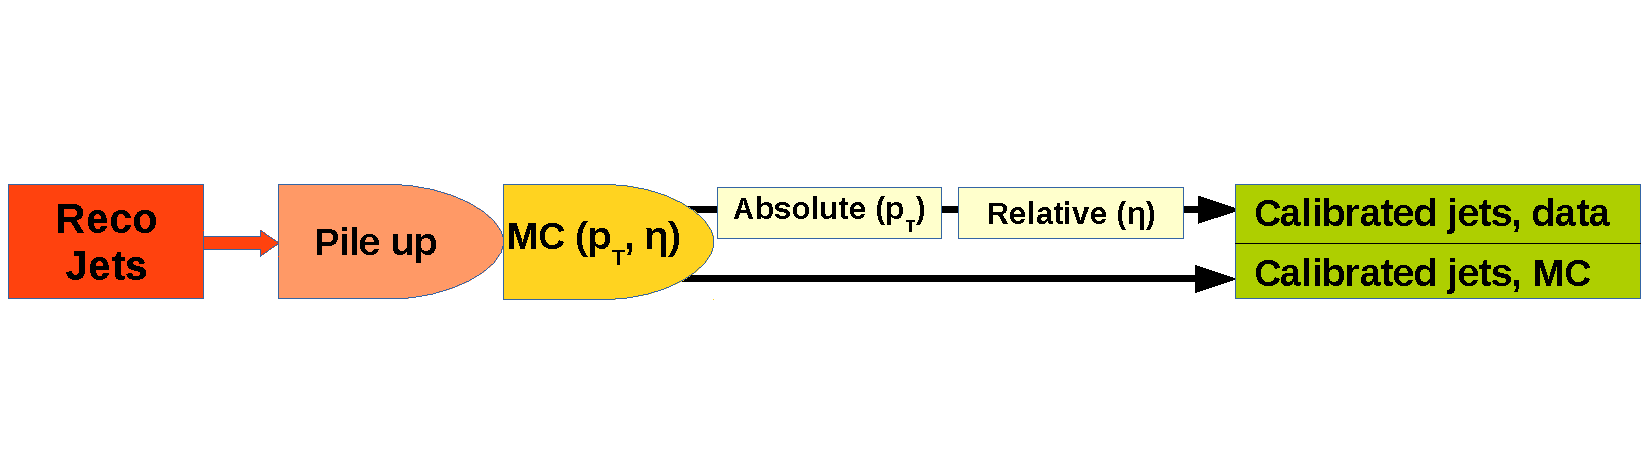
\includegraphics[width=1.0\textwidth]{04_event_reconstruction/plots/JEC.pdf}
%   \caption{Jet calibration steps applied for the detector data and simulated MC samples.}
%   \label{fig:JECsc}
% \end{figure}
% 
% First calibration step deals with the additional energy in the jet which does not occur from a hard process but rather from the detector noise or pile up. 
% Obviously this correction produces the factor always smaller then 1 thus the jet energy reduces on this step. Further correction steps aim to make the jet response
% flat as a function of $|\eta|$ and $p_{T}$. The correction on the geometrical position dependence corrects all the energies as if they were measured 
% in the most efficient barrel region using the dijet data events. The $p_{T}$ dependence correction makes use of the Drell-Yan events to exploit a good
% lepton energy and momentum resolutions. Finally the residual corrections are applied on data to correct for some minor disagreement with the simulation.
% 
% In general all the corrections factor in the kinematic region of interest for this analysis are smaller then $5\%$.
% 
% \subsection{Jet selection}
% 
% This analysis requires only the events where at least two well reconstructed jets are present. All the energies are calibrated as explained in sec.\ref{ssec:JCal}.
% The jets are required to be reconstructed in the barrel region of the detector with the pseudorapidity $|\eta| \leq 2.4$ and with the transverse momentum of at least 
% 30 GeV. 
% 
% \subsection{b-Jets identification}\label{ssec:bTag}
% 
% A jet may arise from any parton, not only from a $b$ quark. But there are some properties which may allow to distinguish a $b$-jet from the other jets. In particular
% a long life time of the B hadrons (in the order of $10^{-12}$ s) allows it to travel far enough from the primary interaction point before the decay. The point
% in space, which corresponds to the place of $B$-hadron decay can be reconstructed in the pixel tracking detector as a \textit{secondary vertex}. The other important
% parameter which can be used to identify the jet origin is the impact parameter of the tracks arising from the secondary vertex. The discussed properties are 
% displayed on the Figure \ref{fig:SV}.
% 
% \begin{figure}[t]
%   \centering
%   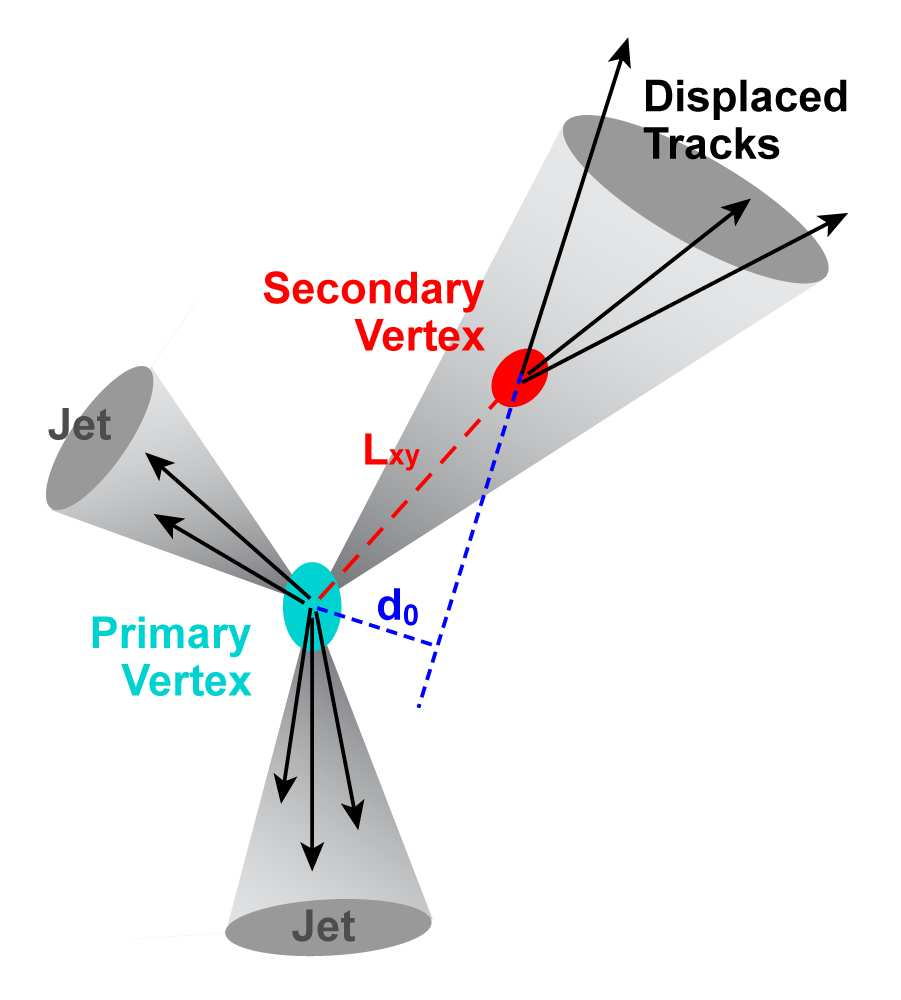
\includegraphics[width=0.5\textwidth]{04_event_reconstruction/plots/btagging_cartoon.png}
%   \caption{A sketch of the event with a reconstructed secondary vertex. A light blue circle is the primary vertex and a red circle is the secondary vertex. The impact 
%   parameter is marked with a blue dashed line and a symbol $d_{0}$.}
%   \label{fig:SV}
% \end{figure}
% 
% The algorithms which aim to find the jets originating from $b$-quarks are called the \textit{b-tagging algorithms}. All of them define a single discriminator value for each jet.
% The algorithms used for the different analyses of the data recored by the CMS detector in 2012 are listed as follows \cite{CMS-PAS-BTV-13-001}: 
% 
% \begin{itemize}
%  \item \textit{Track Counting High Purity} (THCP): the discriminator value is defined as a significance of the impact parameter\footnote{A \textit{significance} is a relation 
%  of the impact parameter value $d$ to it's measurement uncertainty $\sigma_{d}$: $S = \frac{d}{\sigma_{d}}$} of the track with the third highest
%  impact parameter significance;
%  %
%  \item \textit{Jet Probability} (JP): the discriminator is a likelihood value for all associated tracks to arise from the primary vertex. 
%  %
%  \item \textit{Combined Secondary Vertex} (CSV): a likelihood-based discriminator uses the secondary vertex and lifetime information to distinguish $b$-jets, $c$-jets
%  and light jets. This method was exploited for the analyses presented.
% \end{itemize}
% 
% The minimum thresholds for the algorithm are defined as three \textit{working points}, loose (L), medium (M) and tight (T), as following \cite{CMS-PAS-BTV-13-001}:
% 
% \begin{itemize}
%  \item [--] CSVL sets the threshold on the actual discriminator value as $\geq 0.244$, which has an efficiency $\sim 80\%$ and a misidentification probability of
%  light hadron jets close to $10\%$;
%  %
%  \item [--] CSVM sets a harsher threshold on the discriminator value of $\geq 0.679$, which lowers the misidentification probability to $\sim 1\%$, but also
%  reduces the statistics down to 65$\%$;
%  %
%  \item [--] CSVT has the hardest threshold on the discriminator value of $\geq 0.898$. This lowers the misidentification probability by other factor of 10 ($0.1\%$)
%  and reduces the efficiency down to 50$\%$;
% \end{itemize}
% 
% In general the efficiency of the CSV algorithm was estimated in data and simulated QCD events \cite{CMS-PAS-BTV-13-001}. The resulting curve is presenter on the figure \ref{fig:CSVeff}.
% 
% \begin{figure}[t]
%   \centering
%   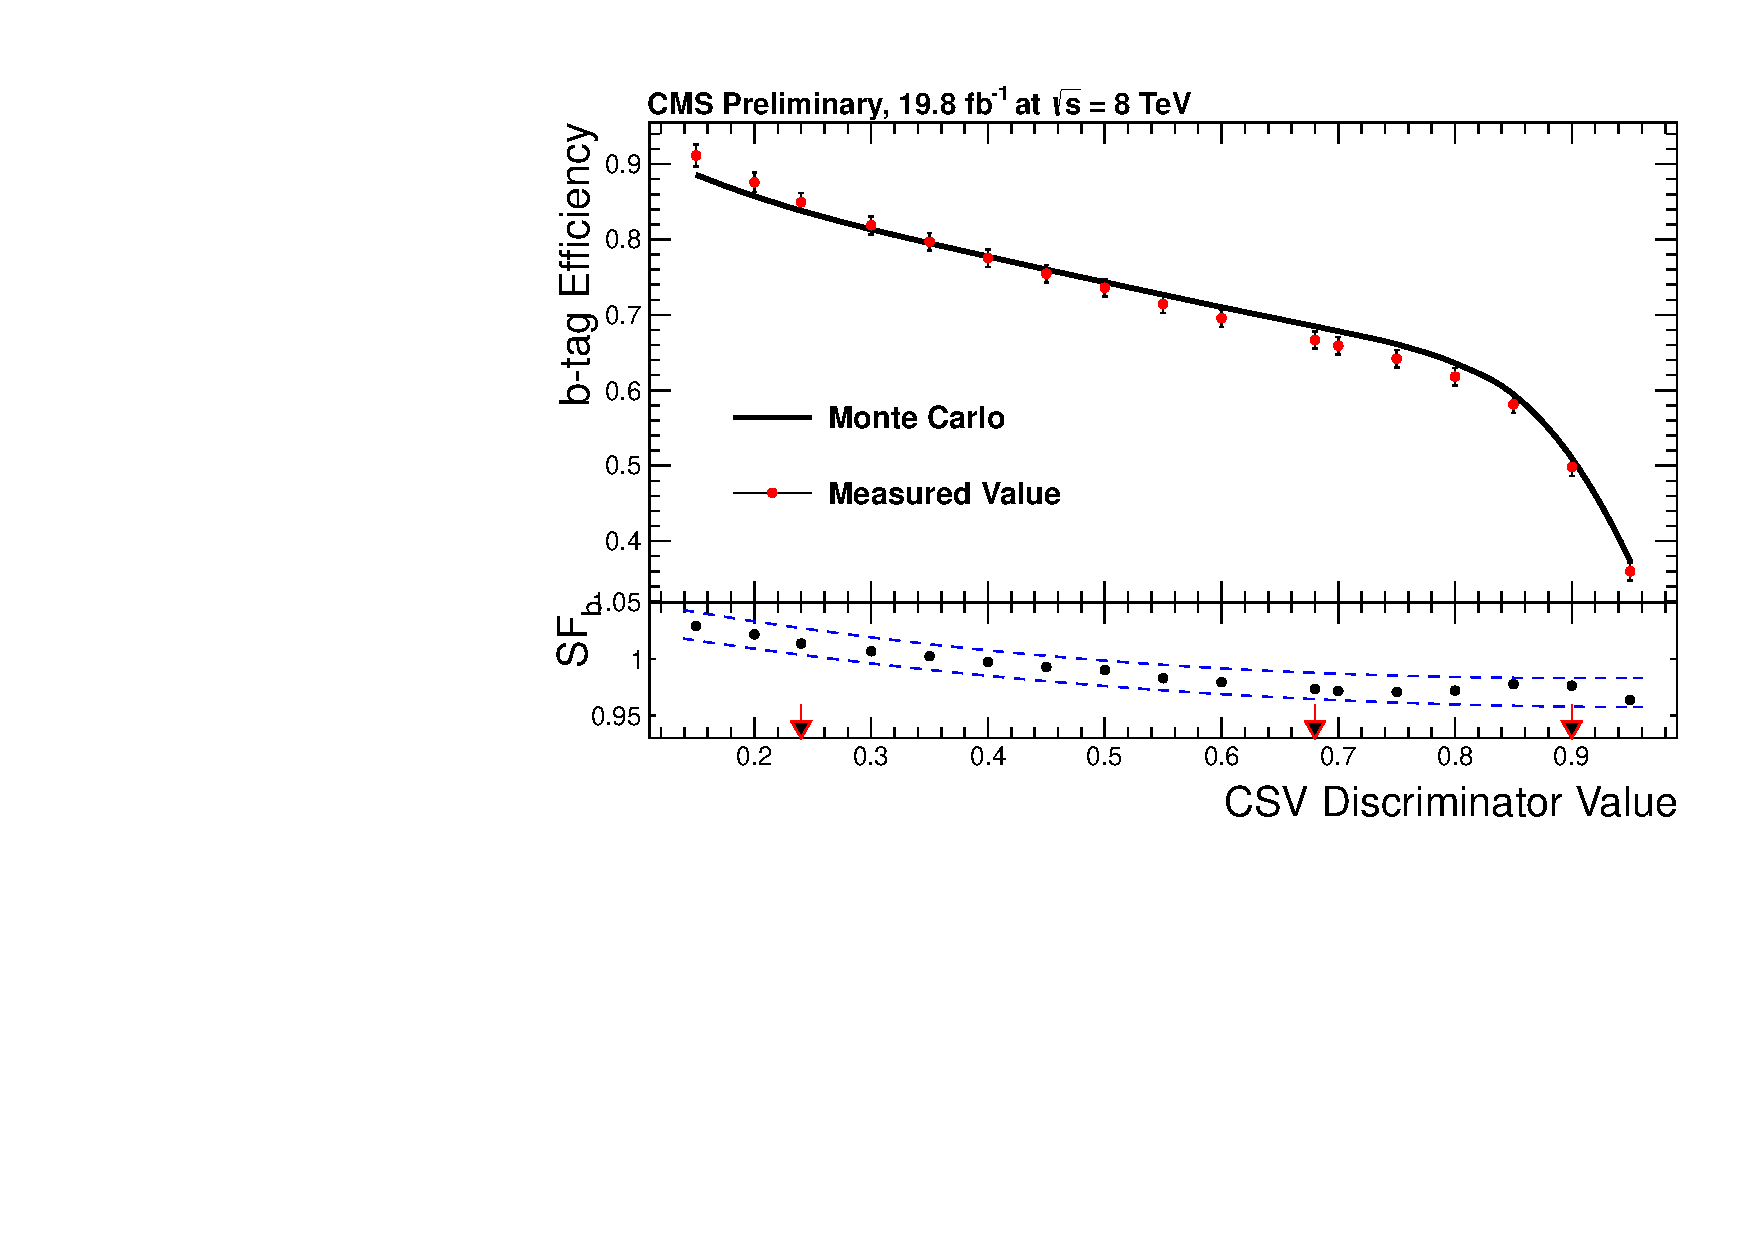
\includegraphics[width=0.6\textwidth]{04_event_reconstruction/plots/Figure_012-b.pdf}
%   \caption{A b-jet tagging efficiency as a function of the discriminator threshold for the CSV algorithm. The upper panel shows the efficiency measured in data and predicted from the simulation.
%   The lower panel shows the ratio between data and simulation efficiencies, where the blue line represents the combined statistical and systematical uncertainty. The plot is taken from \cite{CMS-PAS-BTV-13-001}.}
%   \label{fig:CSVeff}
% \end{figure}
% 
% For this analysis the jets are tagged as arising from a $b$-quark in case they are accepted by CSVL. An event is selected only if it contains at least one $b$-tagged jet.
% 
% \section{Missing Transverse Energy}
% 
% Previously the reconstruction methods and algorithms of all the charged objects of the $t\bar{t}$ dilepton final states were described. However the most complicated 
% task is to reconstruct the two neutrinos which are neutral and don't interact with detector material thus don't provide any direct trace. The only thing to rely on is
% observation of the energy imbalances which may point to the presence of undetected objects. The variable responsible for energy imbalance in the transverse plane is 
% the missing transverse energy $\vec{E^{miss}_{T}}$ (see sec. \ref{sec:CMS}) which is reconstructed using the particle flow algorithm \cite{CMS-PAS-PFT-09-001} (see sec. \ref{sec:PF})
% as a vectorial sum over all reconstructed particles in the event and then taking the opposite of this azimuthal, momentum two-vector. The missing transverse energy is the modulus
% of this vector.
% 
% \begin{align}
%  \vec{E}_{T}^{miss} & = (E_{T_{x}}^{miss}, \, E_{T_{y}}^{miss}) = - \sum_{leptons} \vec{p}_{T}^{lepton} - \sum_{jets} \vec{p}_{T}^{jet}, \\
%  E_{T}^{miss} & = \sqrt{E_{T_{x}}^{miss^{2}} + E_{T_{y}}^{miss^{2}}}.
% \end{align}
% 
% Missing transverse energy reconstruction strongly relies on the quality of leptons and jets reconstruction and is sensitive to the pile up objects. Thus, it is
% crucial to have a precise distinction to the objects from different collisions. To correct for the pile up effects the Multivariate Analysis (MVA) was performed \cite{CMS-PAS-JME-12-002}.
% The MVA is trained on the $Z \to e^{+}e^{-} / \mu^{+}\mu^{-}$ samples and attempts to distinguish between the events emerging from the hard interaction point and
% pile up verteces. The improvement in resolution which the exploiting of the MVA for pile up rejection gives is $\sim 6\%$. However, the differences between data
% and simulation are getting larger. To compensate for these discrepancies the \textit{recoil corrections} are applied \cite{CMS-PAS-JME-12-002}. 
% 
% A recoil $\vec{u}$ is calculated using the well reconstructed $Z \to e^{+}e^{-} / \mu^{+}\mu^{-}$ samples and is defined as shown in the eq. \ref{eq:recoil}:
% 
% \begin{equation}
%  \vec{u} = - \vec{p}_{T}(Z) - \vec{E}_{T}^{miss}
% \end{equation}
% 
% The parallel ($u_{||}$) and perpendicular ($u_{\perp}$) components with respect to the $Z$ direction are simultaneously fitted in data and simulation for each bin
% of the jet multiplicity and $p_{T}(Z)$. The areas of the fit curves $f$ in data and MC simulations are required to be equal:
% 
% \begin{equation}
%  \int_{-\infty}^{u_{corr}} f_{data}\; du = \int_{-\infty}^{u_{uncorr}} f_{sim.}\; du.
% \end{equation}
% 
% The corrected recoil value $u_{corr}$ is used to reestimate the missing transverse energy as $\vec{E}_{T}^{miss} = | \vec{p}_{T}(Z) - \vec{u}_{corr}$.
% 
% For this analysis the events in the $ee$ and $\mu\mu$ channels are accepted only in case the missing transverse energy is $E_{T}^{miss} > 40 \textrm{GeV}$. This rejects
% the background events with a not real missing transverse energy.
% 
% \section{Event Selection Summary}
% 
% The full final state objects selection has been presented and all the selection criteria are summarized as follows:
% 
% \begin{itemize}
%  \item [--] \textbf{Trigger selection}: The events have to be accepted by the dilepton triggers, which require the presents of two leptons, electrons or muons, with
%  minimum transverse momentum of 17 GeV and 8 GeV. 
%  %
%  \item [--] \textbf{Beam scrapping}: Accept only events with maximum 10 reconstructed tracks, or more then 10 in case at least quarter of them has high quality of reconstruction.
%  %
%  \item [--] \textbf{Calorimeter noise removal}: Event with anomalous calorimeter noise are removed.
%  %
%  \item [--] \textbf{Presence of a good vertex}: Events which contain at least one primary vertex with high reconstruction quality are accepted.
%  %
%  \item [--] \textbf{Lepton selection}: An event has to contain at least two leptons with $p_{T} > 20 \textrm{GeV}$ and $|\eta| < 2.4$. Both leptons have to be isolated with 
%  $I_{rel}\leq 0.15$ in a cone of $\Delta R = 0.3$.
%  %
%  \item [--] \textbf{Lepton pair selection}: The mass of the system of two leading $p_{T}$ leptons has to be less then 20 GeV, otherwise the event is rejected. For the
%  same flavour channels a window of $76\textrm{ GeV}\leq m(l\bar{l}) \leq 106\textrm{ GeV}$ is cut out.
%  %
%  \item [--] \textbf{Jet selection}: The events which contain at least two jets with $p_{T} > 30$ GeV and $|\eta| \leq 2.4$ are accepted. Additionally, an event has to contain
%  at least one jet, tagged as originating from the $b$-quark with the help of CSVL.
%  %
%  \item [--] \textbf{Missing Transverse Energy selection}: For the same flavour channels only the events with $E_{T}^{miss} > 40$ GeV are accepted.
% \end{itemize}
% 
% The set of selection criteria performs successfully decreasing the fraction of background events. The control distributions which show the data and MC simulation at one plot
% contain all the background sources as a part of MC, thus providing a visualization of the outcoming results of the event selection process. 

\chapter{Event Selection}\label{chapt:event_sel}
 
This work was aiming to reconstruct the $t\bar{t}$ pair in the dilepton decay channel, or
$t\bar{t} \to W^{+}b\,W^{-}\bar{b} \to \bar{l}b\,l\bar{b}$. Thus the aim is to 
look for the event in the detector with two leptons of the different sign and two jets. The 
neutrino can't be measured directly, their presence is reflected in the non-zero transverse
missing energy $E_{T}^{miss}$. The lowest branching ratio of the dileptonic decay channel
($BR \simeq 4.8\%$) is countervailed by a a precise lepton reconstruction, which can reduce
the fraction of the background events to larger extend.

The reconstructed objects in each event (which corresponds to one bunch crossing) have to fulfill certain 
criteria to be accepted for this analysis. These criteria are chosen taking to account the physical 
result this analysis is aiming for and the technical features of the CMS detector parts.

The imperfect correspondence of the simulation model to the real data has to be additionally 
corrected. The differences in the efficiencies of certain procedures in data and simulation 
are corrected by applying \textit{Scale Factors}, $SF = \frac{\epsilon_{data}}{\epsilon_{MC}}$, 
on the MC distributions. Here $\epsilon_{data}$ is the efficiency determined in the experimental 
data and $\epsilon_{MC}$ is the efficiency from simulation. 

This chapter gives an overview of the $t\bar{t}$ event selection. The 
procedures are based on the CMS Top-Quark-Physics-Analysis group recommendations \cite{TopPAGreco}.
The full chain of event selection are described. 
Resulting event yields are represented in the control distributions, showing the data, simulated signal and backgrounds.

\section{Background Sources}\label{sec:bg_intro}

Not all of these events which have two leptons and two jets in the final state are the \textbf{signal events} 
originating from the $t\bar{t}$ system decay in dileptonic channel. The final state, which can be 
misidentified as $t\bar{t}$, may arise from a different process, called \textit{background}
for the specific measurement. In this analysis the background rates are estimated from the simulation.
The following background processes are discussed in frames of this analysis:

\begin{itemize}
 \item $t\bar{t}\rightarrow$other. This background source includes the other $t\bar{t}$ decay modes (see sec. \ref{ssec:tdecay}).
 \item single top production, which was simulated using \Powheg + \PYTHIA;
 \item Drell-Yan process, which was generated utilizing \PYTHIA. It can be mistreated as $t\bar{t}$ signal, as it also has a dileptonic
 final state signature. However, only the same flavour leptons are produced in Drell-Yan processes. Therefore, the fraction of these
 background events in the $e\mu$ final state is small;
 \item diboson production, simulated using \PYTHIA. These events also have the leptonic final state and may be picked as a $t\bar{t}$
 candidate;
 \item $Z/\gamma^{*} \rightarrow \tau\tau$ production, which was generated using \PYTHIA. Here the $\tau$-leptons decay further
 to $e$, $\mu$ and neutrinos;
 \item $Z/\gamma^{*} \rightarrow ee/\mu\mu$ production, generated using \PYTHIA;
 \item associated $t\bar{t}\;+\; W/Z/\gamma$ production, simulated in \MG + \PYTHIA;
 \item associated $W\;+\;jets$ production, generated using \MG + \PYTHIA;
 \item QCD multijet processes, generated in \PYTHIA.
\end{itemize}

To be able to compare these generated background samples, they were normalized to the data integrated luminosity of 19.7 fb$^{-1}$ and
to their production cross sections\cite{TWikiXSec}.

The selection, which will be introduced in this section, is aiming to distinguish the $t\bar{t}$ events
from the background processes exploiting physical features of each process.

\section{Good Runs}

For the work presented in this thesis the following CMS data samples were used:

\begin{center}\label{tab:samples}
  \begin{tabular}{| c c c |}
    \hline
    \textbf{Samples} & \textbf{Events} & \textbf{Run Range} \\ \hline
    /MuEG/Run2012A-22Jan2013-v1/AOD & 2.5M & 190456 - 193621 \\ 
    /MuEG/Run2012B-22Jan2013-v1/AOD & 15M & 193834 - 196531 \\
    /MuEG/Run2012C-22Jan2013-v1/AOD & 21M & 198022 - 203742 \\
    /MuEG/Run2012D-22Jan2013-v1/AOD & 22M & 203777 -  208686 \\
    \hline
  \end{tabular}
\end{center}

Only the good runs from the LHC certified good run list\cite{JSON} are selected for the analysis out of these data sets.

\section{$t\bar{t}$ Event Selection and Correction}\label{sec:sel}

Various selection criteria and related scale factors are presented in this section.

The results of the selection are presented in the control distributions. These plots show the comparison between the yields in the experimental data and the simulated MC samples.
The various background sources are also presented separately in the distributions. The simulated yields are additionally scaled to the data luminosity of 19.7\;$fb^{-1}$.
All the plots include the statistical uncertainties only.

All the selection requirements are summarized as follows:

\begin{itemize}
 \item [--] \textbf{Trigger selection}: The events have to be accepted by the HLT (see section \ref{sec:trig}) dilepton triggers, which require the presents of two leptons, electrons or muons, with
 minimum transverse momentum of 17 GeV and 8 GeV.
 
 The Scale Factors connected to the trigger selection were applied on the MC double-differentially in bins of the two leptons rapidities. 
 %%%% 
 \item [--] \textbf{Beam scrapping}: Accept only events with maximum 10 reconstructed tracks, or more then 10 in case at least quarter of them has high quality of reconstruction.
 %%%%
 \item [--] \textbf{Calorimeter noise removal}: Event with anomalous calorimeter noise are removed.
 %%%%
 \item [--] \textbf{Vertex requirement}: Events with at least one "good" primary vertex are selected.
 This means that the number of associated tracks should be larger then 4 and a vertex should be positioned centrally in the detector
 \footnote{Only the events with the vertex position $|z| < \textrm{24 cm}$ and $|\rho| < \textrm{2 cm}$ are accepted. All the coordinates
 are given with respect to the CMS coordinate system (see sec.\ref{sec:CMS})}. Only the ``hardest vertex'' 
 (with the highest sum of the $p_{T}^{2}$ of the assigned tracks) is taken for the analysis. 
 \\
 An additional weight correction depending on the event vertex multiplicity is applied on the MC. 
 The distributions presented in the figure \ref{fig:PUweight} show how the agreement
 between the experimental and simulated data improves after this reweighting is implemented.
 
 \begin{figure}[h]
 \centering
 \begin{subfigure}
   \centering
   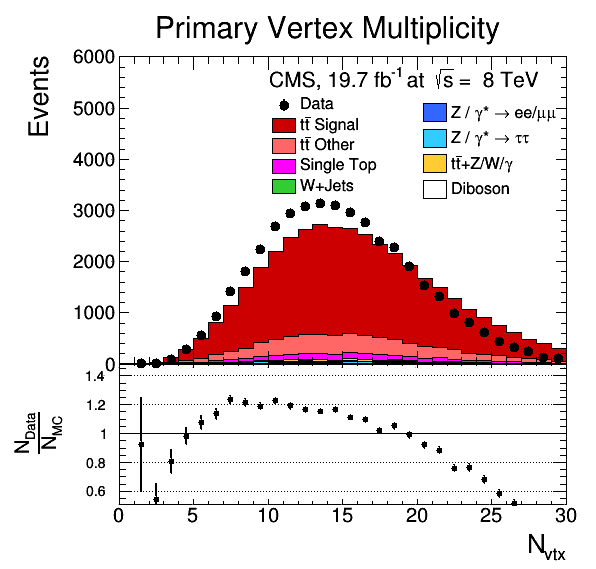
\includegraphics[width=0.49\textwidth]{04_event_reconstruction/plots/vertex_mult_noPUw.png}
 \end{subfigure}
 \begin{subfigure}
   \centering
   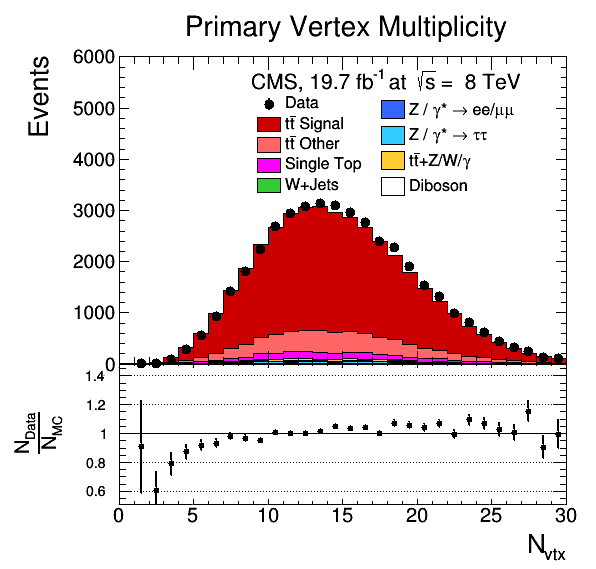
\includegraphics[width=0.49\textwidth]{04_event_reconstruction/plots/vertex_mult_PUw.png}
 \end{subfigure}
 \caption{The vertex multiplicity control distribution before (left) and after (right) the vertex correction reweighing after the full event selection.
 Black dots represent the experimental data and the colored histograms are the MC simulation divided into signal and backgrounds contributions.
 The bottom plots represent the ratio between experimental and simulated data rates.}
 \label{fig:PUweight}
 \end{figure}
 
 %%%%%
 \item [--] \textbf{Lepton isolation}: All the leptons in the event have to be isolated with $I_{rel}\leq 0.15$ in a cone of $\Delta R = \sqrt{\Delta\eta^{2} + \Delta\phi^{2}} = 0.3$ 
 around the lepton track, where $I_{rel}$ is the relative isolation defined as:
  \begin{equation}\label{eq:Iso}
   I_{rel} = \frac{\sum E_{Tracker} + \sum E_{ECAL} + \sum E_{HCAL}}{p_{T}(l)}
  \end{equation}
 
 As it is shown in the figure \ref{fig:PFIso}, the lepton isolation requirement cuts on the events which dominated by the QCD background.

 \begin{figure}[h]
 \centering
 \begin{subfigure}
   \centering
   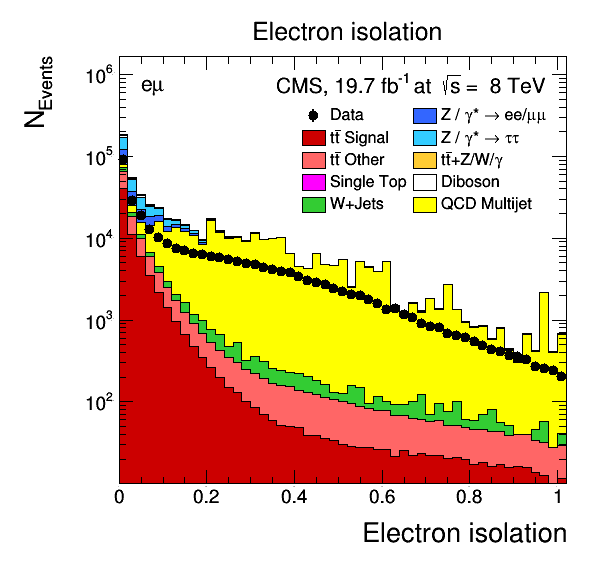
\includegraphics[width=0.49\textwidth]{04_event_reconstruction/plots/PF_e_Iso.png}
 \end{subfigure}
 \begin{subfigure}
   \centering
   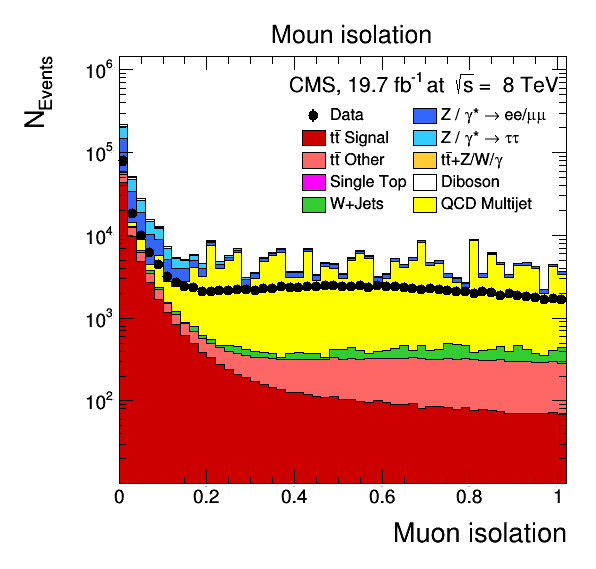
\includegraphics[width=0.49\textwidth]{04_event_reconstruction/plots/PF_mu_Iso.png}
 \end{subfigure}
 \caption{The electron (left) and muon (right) relative isolation $I_{rel}$ (\ref{eq:Iso}) control distributions displaying the experimental data points
 and simulated distributions of signal and different background after the trigger selection. The vertical dashed lines show the isolation cut value.}
 \label{fig:PFIso}
 \end{figure}
 
 The efficiencies of the lepton isolation were determined using \textbf{tag and probe} method \cite{TWikiTP}. The corresponding scale factors are applied on the
 simulation level in bins of $p_{T}$ and $\eta$ of lepton separately for electrons and for muons.
 %%%%%
 \item [--] \textbf{Lepton pair selection}: An event has to contain at least two opposite signed leptons (electron-muon pair) with $p_{T} > 20 \; \textrm{GeV}$ and $|\eta| < 2.4$.
 The invariant mass of the system of the leading $p_{T}$ electron and muon has to be more than 20 GeV, otherwise the event is rejected. 
 %%%%%
 \item [--] \textbf{Jets selection}: Events which contain at least two jets with $p_{T} > 30$ GeV and $|\eta| \leq 2.4$ are accepted. It is natural to expect
 that events with less than two jets will be dominated by Drell-Yan background as the leading order Drell-Yan process does not contain jets in the final state. This is also 
 reflected by the jet multiplicity distribution (Fig. \ref{fig:jetMultiSel}). 
 
 \begin{figure}[h]
  \centering
  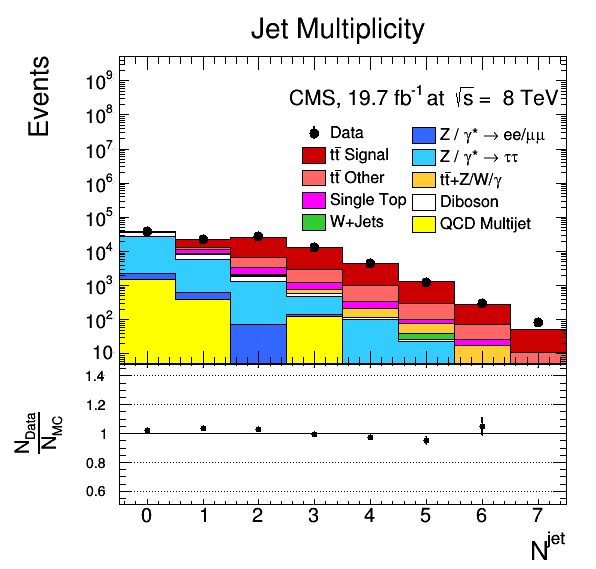
\includegraphics[width=0.6\textwidth]{04_event_reconstruction/plots/JetMulti.png}
  \caption{The control distribution of the jet multiplicity in the events after the trigger and lepton selection. The experimental data points
  and simulated distributions of signal and different backgrounds are plotted. The error bars of the data points
 correspond to the statistical uncertainties of the measurement. The bottom plots represent the data-to-MC yield ratio distributions.}
  \label{fig:jetMultiSel}
 \end{figure}
 
%  In the figure \ref{fig:mllJetSel} the dilepton mass before and after jet selection is shown, demonstrating a sizable background (especially Drell-Yan) fraction suppression power
%  of the cuts implemented in this selection step.
%  
%  \begin{figure}[h]
%  \centering
%  \begin{subfigure}
%    \centering
%    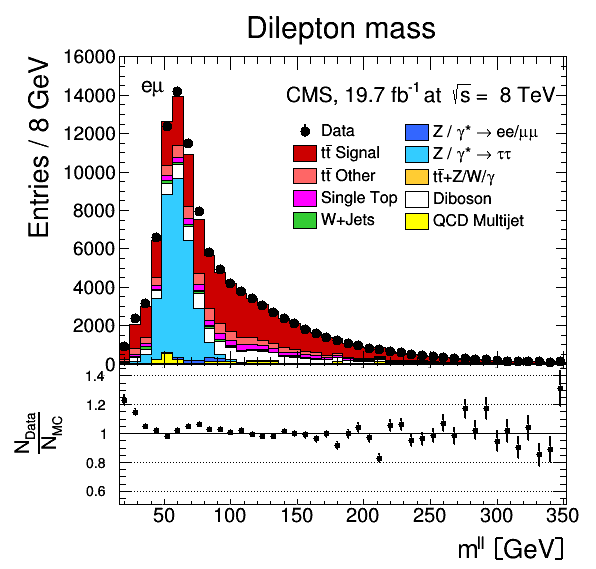
\includegraphics[width=0.49\textwidth]{04_event_reconstruction/plots/mll_step4.png}
%  \end{subfigure}
%  \begin{subfigure}
%    \centering
%    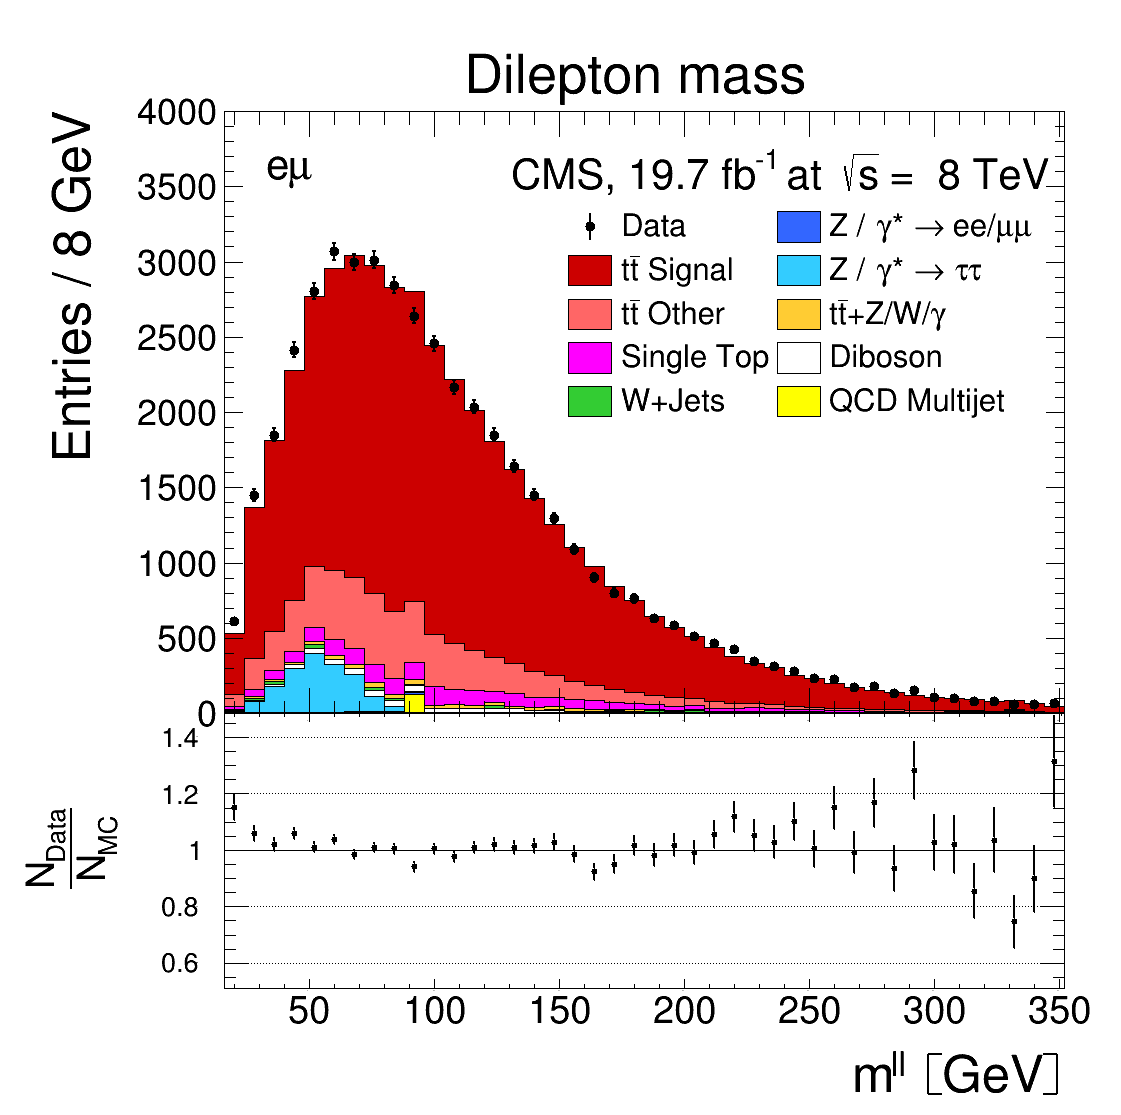
\includegraphics[width=0.49\textwidth]{04_event_reconstruction/plots/mll_step5.png}
%  \end{subfigure}
%  \caption{The control distribution of the dilepton mass in the events after the trigger and lepton selection (left) and after trigger, lepton and jet selection (right). 
%  The experimental data points and simulated distributions of signal and different background are plotted.}
%  \label{fig:mllJetSel}
%  \end{figure}
 %
 \item [--] \textbf{$b$-jets selection}: An event has to contain at least one jet, tagged as originating from the $b$-quark with the b-tagging probability according to the CSVL (sec. \ref{ssec:bTag}). The multiplicity of the $b$-tagged
 jets is presented in the figure \ref{fig:bjetMultiSel} which shows that cutting out the events with no $b$-tagged jets should remove a sizable background fraction. Indeed, the figure \ref{fig:mllbJetSel} presenting
 the dilepton mass before and after the $b$-jets selection shows this background reduction.
 
 \begin{figure}[h]
  \centering
  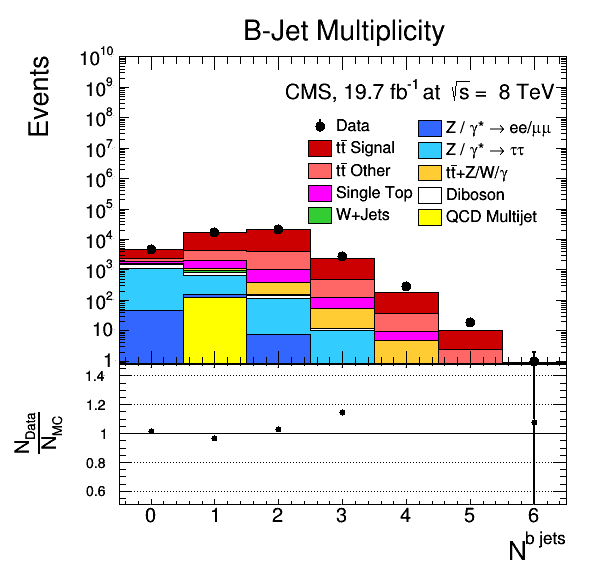
\includegraphics[width=0.6\textwidth]{04_event_reconstruction/plots/bJetMulti.png}
  \caption{The control distribution of the $b$-jet multiplicity in the events after the trigger, lepton and jet selection. The experimental data points
  and simulated distributions of signal and different background are plotted. The error bars of the data points
  correspond to the statistical uncertainties of the measurement. The bottom plots represent the data-to-MC yield ratio distributions.}
  \label{fig:bjetMultiSel}
  \end{figure}
  
 \begin{figure}[h]
 \centering
 \begin{subfigure}
   \centering
   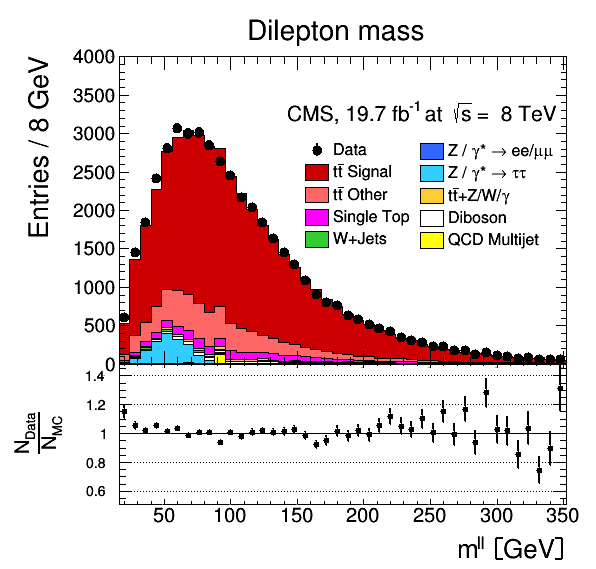
\includegraphics[width=0.49\textwidth]{04_event_reconstruction/plots/mll_step6.png}
 \end{subfigure}
 \begin{subfigure}
   \centering
   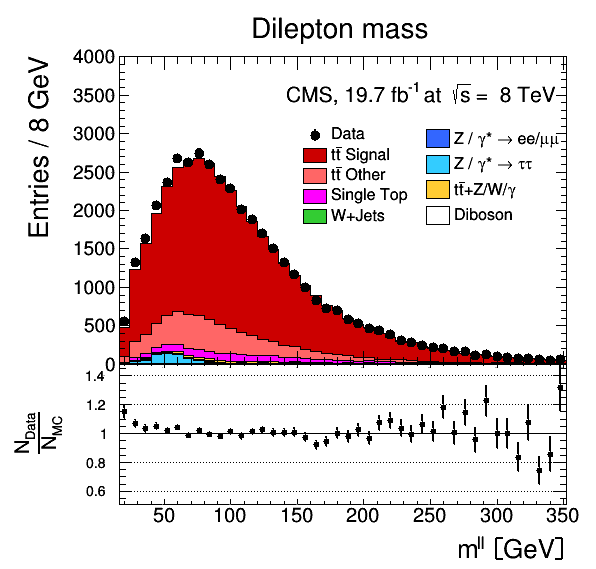
\includegraphics[width=0.50\textwidth]{04_event_reconstruction/plots/mll_step7.png}
 \end{subfigure}
 \caption{The control distribution of the dilepton mass in the events after the trigger, lepton and jet selection (left) and after applying in addition the $b$-jet selection (right). 
 The experimental data points and simulated distributions of signal and different background are plotted. The error bars of the data points
 correspond to the statistical uncertainties of the measurement. The bottom plots represent the data-to-MC yield ratio distributions.}
 \label{fig:mllbJetSel}
 \end{figure}
 
 The scale factors corresponding to the $b$-tagging procedure were applied on the MC improving much the agreement between data and simulation. This effect can be seen in the 
 figure \ref{fig:bTagDiscr}, which presents the CSV discriminator distribution before and after the $b$-tagging SF reweighing. The data-to-MC ratio plots are getting closer to one with
 applying the SFs.
 
 \begin{figure}[h]
 \centering
 \begin{subfigure}
   \centering
   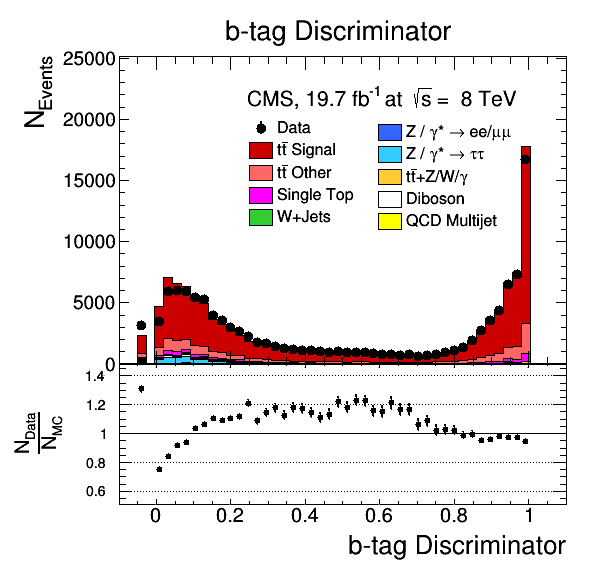
\includegraphics[width=0.49\textwidth]{04_event_reconstruction/plots/bTagDiscr_step6.png}
 \end{subfigure}
 \begin{subfigure}
   \centering
   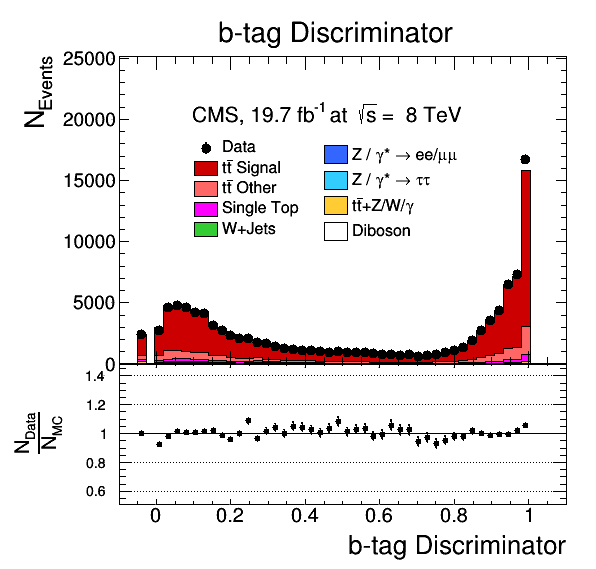
\includegraphics[width=0.49\textwidth]{04_event_reconstruction/plots/bTagDiscr_step7.png}
 \end{subfigure}
 \caption{The control distribution of the $b$-tag discriminator in the events after the full even selection (\ref{sec:sel}) not applying the $b$-tag Scale Factors (left)
 and after applying the $b$-tag Scale Factors (right). The experimental data points and simulated distributions of signal and different background are plotted.
 The error bars of the data points correspond to the statistical uncertainties of the measurement.
 The bottom plots represent the data-to-MC yield ratio distributions.}
 \label{fig:bTagDiscr}
 \end{figure}
 %
 \end{itemize}

The applied selection criteria dramatically reduced the fraction of background events.

\section{Control Distributions}

The results of the reconstruction and selection described above can be illustrated by control distributions of the objects which are reconstructed for the $t\bar{t}$
final state definition.

The figure \ref{fig:CPetaptLep} shows the lepton $\eta$ and $p_{T}$. An overall reasonable agreement between the data and simulation shapes is observed in all $\eta$ regions
and $p_{T}$'s. The control distribution of the mass of the dilepton (electron-muon) system is shown in figure \ref{fig:CPmll}. The simulation and experimental data
agree well within the statistical uncertainties except for the first bin where data are higher than simulation.

 \begin{figure}[h]
 \centering
 \begin{subfigure}
   \centering
   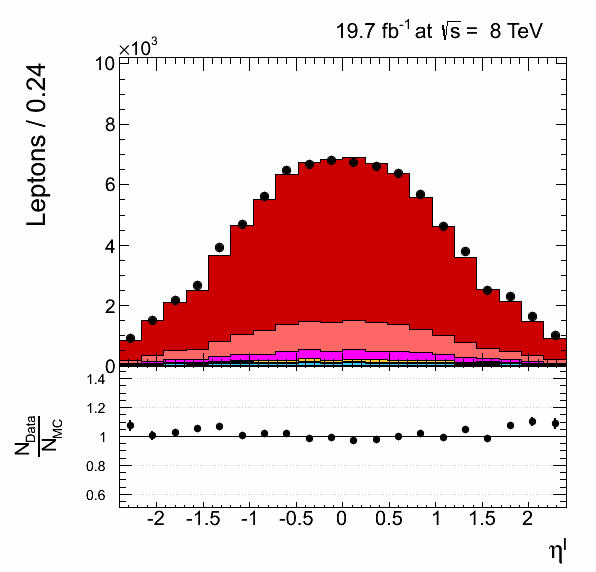
\includegraphics[width=0.49\textwidth]{04_event_reconstruction/plots/basic_lepton_eta_step7.png}
 \end{subfigure}
 \begin{subfigure}
   \centering
   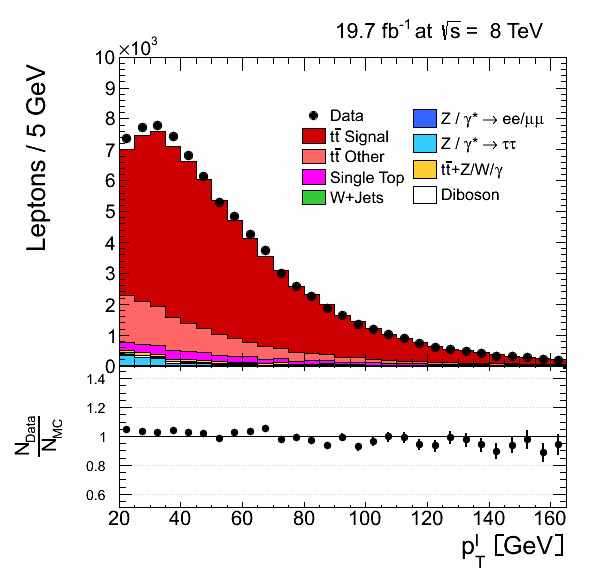
\includegraphics[width=0.49\textwidth]{04_event_reconstruction/plots/basic_lepton_pt_step7.png}
 \end{subfigure}
 \caption{The control distribution of lepton $\eta$ (left) and lepton $p_{T}$ (right) in the events after the whole event selection (\ref{sec:sel}). 
 The experimental data points and simulated distributions of signal and different background are plotted. The error bars of the data points
 correspond to the statistical uncertainties of the measurement. The bottom plots represent the data-to-MC yield ratio distributions. 
 Each distribution has two entries per event - for the electron and for the muon.}
 \label{fig:CPetaptLep}
 \end{figure}
 
 \begin{figure}[h]
  \centering
  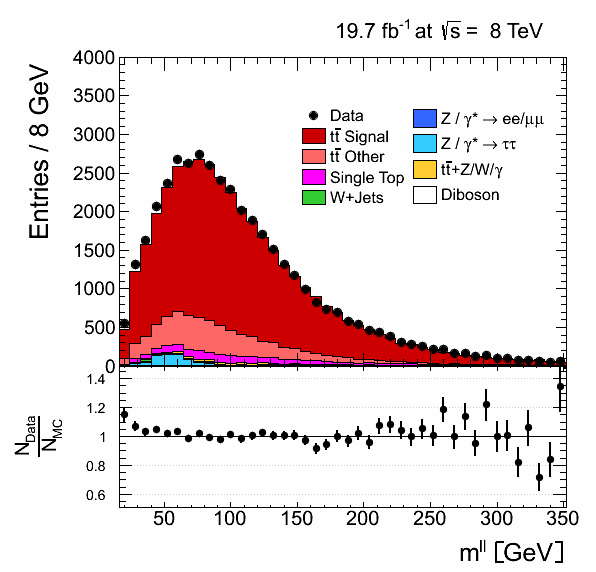
\includegraphics[width=0.6\textwidth]{04_event_reconstruction/plots/basic_dilepton_mass_step7.png}
  \caption{The control distribution of the mass of the electron-muon system in the events after the whole \ref{sec:sel} selection. 
  The experimental data points and simulated distributions of signal and different background are plotted. The jets $p_{T}$ and multiplicity 
  distributions are presented in the logarithmic scale. The error bars of the data points
  correspond to the statistical uncertainties of the measurement. The bottom plots represent the data-to-MC yield ratio distributions.}
  \label{fig:CPmll}
 \end{figure}
 
The kinematics of the reconstructed and selected jets is presented in the figure \ref{fig:CPjetskin} which shows the control distributions for the
jets $\eta$, $p_{T}$ and the jet multiplicity in the events. The simulation describes better the central rapidity ranges. For the jet multiplicities
smaller than 5 a good agreement between experimental data and MC is observed.
 
 \begin{figure}[h]
 \centering
 \begin{subfigure}
   \centering
   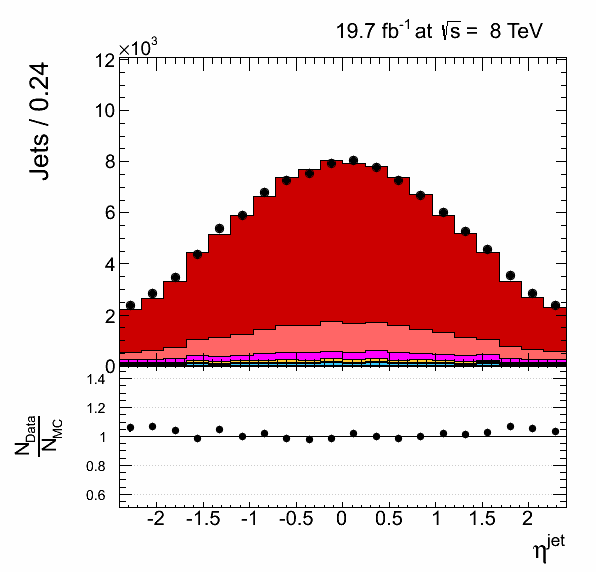
\includegraphics[width=0.49\textwidth]{04_event_reconstruction/plots/basic_jet_eta_step7.png}
 \end{subfigure}
 \begin{subfigure}
   \centering
   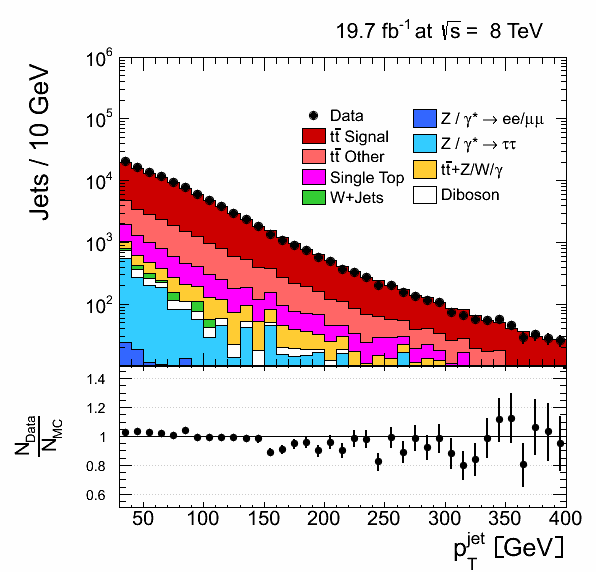
\includegraphics[width=0.49\textwidth]{04_event_reconstruction/plots/basic_jet_pt_step7.png}
 \end{subfigure}
  \begin{subfigure}
   \centering
   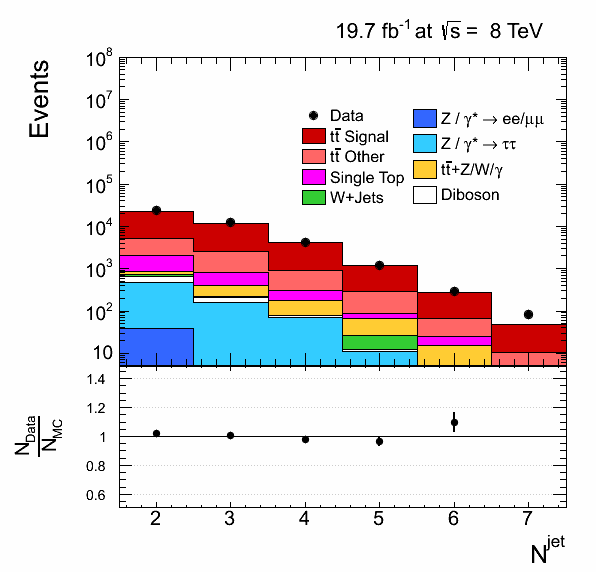
\includegraphics[width=0.49\textwidth]{04_event_reconstruction/plots/basic_jet_multiplicity_step7.png}
 \end{subfigure}
 \caption{The control distribution of the jet $\eta$ (top left) and jet $p_{T}$ (top right) and jet multiplicity in the events 
 after the whole \ref{sec:sel} selection. The experimental data with the error bars corresponding to the statistical uncertainties
 and simulated distributions of signal and different background are plotted. The bottom plots represent the data-to-MC yield ratio distributions. 
 The top distributions have multiple entries per event, corresponding to all reconstructed jets.}
 \label{fig:CPjetskin}
 \end{figure}
 
The multiplicity for the $b$-tagged jets is presented in figure \ref{fig:CPbJetMult} which shows a good agreement for the multiplicities smaller than 4.

 \begin{figure}[h]
  \centering
  \includegraphics[width=0.6\textwidth]{04_event_reconstruction/plots/basic_bjet_multiplicity_step7.png}
  \caption{The control distribution of the $b$-tagged jets multiplicities in the events after the whole \ref{sec:sel} selection. 
  The experimental data points and simulated distributions of signal and different background are plotted in the logarithmic scales. 
  The error bars of the data points correspond to the statistical uncertainties of the measurement. 
  The bottom plots represent the data-to-MC yield ratio distributions.}
  \label{fig:CPbJetMult}
 \end{figure}
 
The control distributions are signal dominated which shows a good performance of the criteria for the $t\bar{t}$ final state selection.





\chapter{Reconstruction of the $t\bar{t}$ Kinematics}\label{chapt:kinReco}

As presented in previous chapter, the two neutrinos are not detected and only their transverse energy can be measured. Thus additional
assumptions are needed to define the full final state kinematics of the $t\bar{t}$ decay products.

This section describes a method used for the kinematic reconstruction of $t\bar{t}$ in the dilepton final state. A mathematical
background (sec. \ref{sec:MatBg}) as well as a performance description of the method (sec. \ref{sec:SolSer} -- \ref{sec:kinRecPerf}) are revealed.

\section{Mathematical Background}\label{sec:MatBg}

The problem of two not fully reconstructed neutrinos can be solved by setting certain constrains:

\begin{itemize}
 \item \textit{t and $\bar{t}$ masses} are assumed to be equal and constrained to the same value of 172.5 GeV\cite{PDG-2012};
 \item The whole missing transverse energy $E_{T}^{miss}$ of the event is assumed to arise entirely
 from the two neutrinos from the $t\bar{t}$ decay;
 \item \textit{The $W^{\pm}$ masses} are assumed to be equal and constrained to the value which is randomly taken
 from the generator $W^{\pm}$ mass spectrum.
\end{itemize}

These assumptions lead to the system of six equations with six unknowns (three momentum components of two neutrinos).
The equations are written down assuming the CMS coordinate system (see sec. \ref{sec:CMS}):

\begin{align}\label{alg:LS1}
 E^{miss}_{T_{x}} & =  p_{\nu_{x}} + p_{\bar{\nu}_{x}} \\
 %
 E^{miss}_{T_{y}} & =  p_{\nu_{y}} + p_{\bar{\nu}_{y}} \\
 %
 m^{2}_{W^{+}} & = (E_{l^{+}} + E_{\nu})^{2} - (p_{l^{+}_{x}} + p_{\nu_{x}})^{2} - (p_{l^{+}_{y}} + p_{\nu_{y}})^{2} - (p_{l^{+}_{z}} + p_{\nu_{z}})^2 \\
 %
 m^{2}_{W^{-}} & = (E_{l^{-}} + E_{\bar{\nu}})^{2} - (p_{l^{-}_{x}} + p_{\bar{\nu}_{x}})^{2} - (p_{l^{-}_{y}} + p_{\bar{\nu}_{y}})^{2} - (p_{l^{-}_{z}} + p_{\bar{\nu}_{z}})^2 \\
 % 
 m_{t}^{2} & = (E_{b} + E_{l^{+}} + E_{\nu})^{2} - (p_{b_{x}} + p_{l^{+}_{x}} + p_{\nu_{x}})^2 \nonumber \\
           & - (p_{b_{y}} + p_{l^{+}_{y}} + p_{\nu_{y}})^2 - (p_{b_{z}} + p_{l^{+}_{z}} + p_{\nu_{z}})^2 \\
 %
 m_{\bar{t}}^{2} & = (E_{\bar{b}} + E_{l^{-}} + E_{\bar{\nu}})^{2} - (p_{\bar{b}_{x}} + p_{l^{-}_{x}} + p_{\bar{\nu}_{x}})^2 \nonumber \\
                 & - (p_{\bar{b}_{y}} + p_{l^{-}_{y}} + p_{\bar{\nu}_{y}})^2 - (p_{\bar{b}_{z}} + p_{l^{-}_{z}} + p_{\bar{\nu}_{z}})^2\label{alg:LS6} 
\end{align}

Here the the $E_{l^{\pm}}$ and $p_{l^{\pm}_{x,y,z}}$ correspond to the lepton(antilepton) energy and momentum components respectively; 
$E_{b/\bar{b}}$ and $p_{b/\bar{b}_{x,y,z}}$ are the $b$/$\bar{b}$-jet energy and momentum components respectively; the $E^{miss}_{T_{x,y}}$ are
the two components of the missing transverse energy.
These are the characteristics of the reconstructed objects from the detector information directly, as described in the chapter \ref{chapt:event_selection}.
The six unknowns are the neutrino momentum components $p_{\nu/\bar{\nu}_{x,y,z}}$ and the neutrino energies are just composed from momenta:

\begin{equation}
 E_{\nu/\bar{\nu}}^{2} = p_{\nu/\bar{\nu}_{x}}^{2} + p_{\nu/\bar{\nu}_{y}}^{2} + p_{\nu/\bar{\nu}_{z}}^{2}
\end{equation}

The analytical solution of the system of equations (\ref{alg:LS1}--\ref{alg:LS6}) was proposed in \cite{LSpaper}. After a number of transformations
the system is reduced to one equation:

\begin{equation}\label{eq:eqLSf}
 0 = h_{0} p_{\nu_{x}}^{4} + h_{1} p_{\nu_{x}}^{3} + h_{2} p_{\nu_{x}}^{2} + h_{3} p_{\nu_{x}} + h_{4},
\end{equation}

where the coefficients $h_{0} -- h_{4}$ are described in \cite{LSpaper, LSerrat}. They depend on the four-momenta of the reconstructed 
leptons and jets and also on the missing transverse energy $E_{T}^{miss}$. 

The equation \ref{eq:eqLSf} is a fourth order polynomial. In the ideal case after solving it as described in \cite{LSpaper} one gets
in 80$\%$ of the cases two solutions and in 20$\%$ of the cases -- four solutions, as shown on the figure \ref{fig:LSNsol}.

\begin{figure}[t]
  \centering
  \includegraphics[width=0.6\textwidth]{05_kinReco/plots/medium.png}
  \caption{Number of solutions of the equation \ref{eq:eqLSf}. The distribution is normalized to one. The generated data used for this check
  is produced before any radiation. The figure is taken from \cite{LSpaper}.}
  \label{fig:LSNsol}
\end{figure}

Under the real conditions a sizable amount of the events will find no solutions of the kinematic equations (\ref{alg:LS1}--\ref{alg:LS6})
because of an imperfect reconstruction of the detector objects. But in the other cases there is a possibility to find up to four solutions.

\section{Solution Search}\label{sec:SolSer}

There are several problems arising during the $t\bar{t}$ kinematics reconstruction. A trace to some of them was already given in the previous
section. Following challenges have to be dealt:

\begin{itemize}
 \item \textit{Measurement fluctuations}. As mentioned in section \ref{sec:MatBg}, there might be no solutions found for a certain combination
 of leptons, jets and missing transverse energy if some of them are inaccurately reconstructed and due to some measurement fluctuations the equation
 is lead to an unphysical region.
 %
 \item \textit{Multiple solutions of the kinematic equations}. As discussed in section \ref{sec:MatBg} the solution of the equation \ref{eq:eqLSf}
 provides up to four correct solutions while a real neutrino has only one momentum.
 %
 \item \textit{Multiple combinations of leptons and jets}. An event with a $t\bar{t}$ decaying to a dilepton final state has minimum two leptons and two
 jets. But there is no sign if a jet comes from $t$ or a $\bar{t}$. For this reason each jet is being paired to one of the leptons, and then to another
 to form a $t$ or $\bar{t}$ candidate. Thus an event with two leptons and two jets has two possible $t\bar{t}$ candidates. In case of multiple jets
 in the event, the number of $t\bar{t}$ will be $N_{jet}!$, where $N_{jet}$ is a jet multiplicity. Specifically for this analysis only those combinations 
 of two jets with lepton and antilepton are accepted where at least one jet is b-tagged as discribed in sec. \ref{ssec:bTag}.
\end{itemize}

The last two challenges have different nature but boths cause the same issue of multiple possible $t\bar{t}$ candidates, thus they can be treated together.

\subsection{Measurement fluctuations}

The challenge of rescuing the events which are lost due to the measurement fluctuations can be solved by varying the measured objects energies and
momentum directions. That would increase a chance of pushing the kinematics back to physical region. This idea was implemented by reconstructing
each event 100 times, each time shifting relevant observables randomly according to their resolution determined from the Monte Carlo.

The lepton and jet energies and directions were smeared. All the variations are done simultaneously for every lepton and jet.
The energy variation was performed through multiplication of an actual reconstructed energy value
by a correction factor $f(E) = \frac{E_{reco}}{E_{true}}$. Here the $E_{reco}$ is the lepton or jet energy taken from the MC signal the reconstruction
and the $E_{true}$ is the true energy of the same object on the particle level. The distributions for the $f(E)$ which are used for the random choice
of the correction factors are shown on the Figure \ref{fig:fE}. The shape of these distributions is energy independent (see Appendix !!!), thus they are obtained in
the complete kinematic region. The correction factors which enter the distributions \ref{fig:fE} are determined from the signal MC simulation jets and 
leptons matched to the particle level $b$-quarks and leptons arising from the top decay. 

\begin{figure}[t]
\centering
\begin{subfigure}
  \centering
  \includegraphics[width=0.48\textwidth]{05_kinReco/plots/fE_jet.png}
\end{subfigure}
\begin{subfigure}
  \centering
  \includegraphics[width=0.48\textwidth]{05_kinReco/plots/fE_lep.png}
\end{subfigure}
\caption{Distributions of the energy correction factors used for the energy smearing in the kinematic
reconstruction of the top-quark kinematics. The factor distribution for jets is shown on the left and for
the leptons -- on the right.}
\label{fig:fE}
\end{figure}

Additionally to the energy variation a random gaussian smearing in a random direction around the nominal direction is applied. The resolutions for
the gaussians are taken from the MC distributions presented on the Figure \ref{fig:dAngle}. These distributions are also independent of leptons and
jets kinematics (see Appendix !!!) and thus the resolution applied for smearing is averaged over the whole kinematic range.

\begin{figure}[t]
\centering
\begin{subfigure}
  \centering
  \includegraphics[width=0.48\textwidth]{05_kinReco/plots/dan_jet.png}
\end{subfigure}
\begin{subfigure}
  \centering
  \includegraphics[width=0.48\textwidth]{05_kinReco/plots/dan_lep.png}
\end{subfigure}
\caption{Distributions of the angle between the particle level direction and the detector level direction.
The angle distribution for the b quarks is shown on the left and for the leptons -- on the right.}
\label{fig:dAngle}
\end{figure}

In each of the 100 jet and lepton kinematics variations the transverse missing energy $E_{T}^{miss}$ has to be recalculated. This is done
assuming the transverse energy component, which does not refer to the leptons and jets forming a $t\bar{t}$ candidate, to be constant. Thus,
missing transverse energy for the $i^{th}$ smearing will be expressed as following:

\begin{equation}
 E^{miss\;i}_{T_{x,y}} = E^{miss \; from \, reconstruction}_{T_{x,y}} + p^{jet \; not\,smeared}_{x,y} + p^{lepton\;not\,smeared}_{x,y} - (p^{jet\;i}_{x,y} + p^{lepton\;i}_{x,y})
\end{equation}

\subsection{Single solution choice}

The equation \ref{eq:eqLSf} is solved for every of the 100 event reconstructions. Each equation may have up to four solutions, thus each event
has up to ($100 \otimes 4 \otimes N_{jet}!$) reconstructed $t\bar{t}$ candidates ($N_{jet}!$ component has already been discussed is sec. \ref{sec:SolSer}). 
To obtain one $t\bar{t}$ pair out of this candidate variety, following steps are undertaken:

\begin{itemize}
 \item [--] For each of the four solutions of the equation \ref{eq:eqLSf} the invariant of the $t\bar{t}$ pair, $m(t\bar{t})$, is calculated. Only
 the solution which has the smallest $m(t\bar{t})$ is taken. This criterion was prior introduced in \cite{PhysRevD.73.112006}, where it was shown to
 deliver for the correct lepton-jet assignment in most cases the correct solution.
 %
 \item [--] To the rest of up to ($100 \otimes N_{jet}!$) candidates a weight $\omega = \omega_{m^{\bar{l}b}} \dot \omega_{m^{l\bar{b}}}$
 is calculated. Here $m^{\bar{l}b}$ and $m^{l\bar{b}}$ are the reconstructed invariant masses of the lepton-jet pairs from the top and the anti-top 
 decays, respectively. These weights are calculated from the spectrum of the lepton-jet pairs in top decays obtained from a signal MC on the 
 particle level after all kinematic cuts described in chapter \ref{chapt:event_selection}. A $t$ ($\bar{t}$) momentum is constructed as a wighted 
 average of all smeared solutions as following:
 \begin{equation}
  \langle{\vec{p}(t,\bar{t})}\rangle = \frac{\sum\limits_{i=1}^{100} \omega_{i} \vec{p(t,\bar{t})}_i}{\sum\limits_{i=1}^{100} \omega_i}.
 \end{equation}
 Here $\omega_i$ is a weight and $\vec{p(t, \bar{t})}_{i}$ is a $t$ or $\bar{t}$ momentum three vector for the $i^{th}$ variation in the event. 
 In case no solution of kinematic equations is found, both, weight and momentum three vector are set to zero. To complete the system kinematics,
 the $t$ and $\bar{t}$ energies are calculated taking $\langle{\vec{p}(t,\bar{t})}\rangle$ and assuming the top mass $m(t) = m(\bar{t}) = $ 172.5 GeV.
\end{itemize}

\section{Performance}\label{sec:kinRecPerf}

Only the events in which the solution of kinematic equations is found are accepted for this analysis. Thus it is important to study the efficiency
of the kinematic reconstruction method proposed. Figure \ref{} shows the efficiency depending on jet multiplicity in the event. A slight efficiency
drop can be explained by the increase of number of possible $t\bar{t}$ candidates in the event due to multiple combinations of leptons and jets
(see sec. \ref{sec:SolSer}). An integrated efficiency of the kinematic reconstruction method is 93 $\%$.

The kinematic reconstruction method proposed shows desirable results over the complete kinematic range of the top system. As shown on the Figure \ref{} 
$t\bar{t}$ pairs are reconstructed up to the higher edges of pseudorapidity and transverse momentum. In general, a good agreement between data and
simulation results is observed. Signal is dominating backgrounds in all the bins of kinematic observables.

The scatter plots on Figure \ref{} show the correlation between the kinematic variables after the selection and kinematic reconstruction in the simulated
signal and the actual characteristics of the $t\bar{t}$ system and decay on the particle level. There are no shifts and trends observed, thus showing 
the trustful behavior of the kinematic reconstruction algorithm.

% \subsection{Efficiency Studies}
% \subsection{Control Distributions}
% \subsection{Quality Studies}


\chapter{Cross Section Measurement}

The cross section measurement procedure and results are explained in this section.
After applying selection criteria and kinematic reconstruction, one can count the events to determine
the rate of $t\bar{t}$ production process.

The cross sections were measured double differentially in bins of the kinematic variables of top-quark and $t\bar{t}$ system.
The first section gives an overview of the background processes for the $t\bar{t}$ production.
The two dimensional unfolding was applied to correct for the detector effect and fluctuations, which is described
in the second section of this chapter.
The double differential cross sections and their definitions are shown in the last section of the chapter.
% \section{Selection of Binning}\label{sec:binning}

\section{Background Subtraction}
This study is performed as counting the events which fulfill certain criteria (e.g. given in chapter \ref{chapt:event_selection} and 
chapter \ref{chapt:kinReco}). Not all of these events are the \textbf{signal events} originating from the $t\bar{t}$ system decay in dileptonic
channel. The final state, which can be misidentified as $t\bar{t}$, may arise from a different process, called \textit{background}
for the specific measurement. In this analysis the background rates are estimated from the simulation and Subtracted 
from the measured event yields:

\begin{equation}\label{eq:bgsub}
 N^{signal\;measured}_{reco} = N^{selected}_{reco} - N^{BG}
\end{equation}

Here the $N^{BG}$ corresponds to the number of background events. It consists of several processes like:

\begin{itemize}
 \item single top production;
 \item Drell-Yan process;
 \item diboson production;
 \item associated $t\bar{t}\;+\; W/Z/\gamma$ production;
 \item associated $W\;+\;jets$ production;
 \item QCD multijet processes.
\end{itemize}

Whereas all the background yields are only simulated, the rate of the background caused by the Drell-Yan production is 
partially data driven \cite{Chatrchyan:2011nb}. The normalization factor for the simulated Drell-Yan events is determined 
from the comparison of the reconstructed and simulated $Z$-peak. 

After subtracting all the other backgrounds, the number of signal events is multiplied by the factor to cancel the contribution
from the other decay channels of $t\bar{t}$:

\begin{equation}\label{eq:bgsub}
 N^{signal}_{reco} = N^{signal\;measured}_{reco} \cdot \frac{N^{t\bar{t} \rightarrow e\mu}_{reco}}{N^{t\bar{t} \rightarrow e\mu}_{reco} + N^{t\bar{t} \rightarrow other}_{reco}}.
\end{equation}

%%%%%%%%%%%%%%%%%%%%%%%%%%%%%%%%%%%%%%%%%%%%
%%%%%%%%%%%%%%%%%%%%%%%%%%%%%%%%%%%%%%%%%%%%
%%%%%%%%%%%%%%%%%%%%%%%%%%%%%%%%%%%%%%%%%%%%
\section{Unfolding of the Experimental Results}\label{sec:unfold}

The events after the background  subtraction \ref{eq:bgsub} are grouped to the bins in different variables. However, a finite precision
due to inevitable detector effects and imperfect reconstruction algorithms may lead to incorrect measurement of kinematic properties of the event.
Thus, some fraction of events may be reconstructed in the wrong bins. To present the results independent of the detector effects,
one needs to correct them back.

The whole problem can be described as

\begin{equation}\label{eq:UnfoldProb}
 \tilde{y}_i = \sum_{j = 1}^{m} A_{ij}\tilde{x}_{j} + b_{i}, \;\;\; 1 \leq i \leq n.
\end{equation}

Here the $\tilde{x}_j$ in $m$ bins is a true distribution, independent of the detector effects, which is the aim of the measurement;
$\tilde{y}_i$ in $n$ bins is a distribution which one gets out of the detector and $A_{ij}$ is a matrix of probabilities describing 
the migrations to different bins on the detector level; $b_{i}$ is the background in the bin $i$. 
However, the observed event counts $y_{i}$ may be different from $\tilde{y}_{i}$ due to the statistical fluctuations.
The schematic view of the problem is given in the Figure \ref{fig:scUnf}.

\begin{figure}[t]
  \centering
  \includegraphics[width=0.4\textwidth]{06_DiffXsec/plots/d12-129f1.png}
  \caption{Schematic view of the problem of migration effects due to the finite precision of the detector and statistical 
  fluctuations. Plot taken from \cite{Schmitt:2012kp}.}
  \label{fig:scUnf}
\end{figure}

The process of restoring the true distribution $\tilde{x}_{j}$ from the known distribution $y_{i}$ which was influenced
by the detector effects and statistical fluctuations is called \textit{unfolding}. To minify these fluctuations the 
\textit{regularisation} procedure is applied. The TUnfold \cite{Schmitt:2012kp} algorithm was used for the
unfolding in this analysis.

\subsection{TUnfold Minimization}\label{ssec:TUmini}

The TUnfold algorithm is using the least square minimization method and the Tikhonov regularization \cite{Tikhonov:1963}. One of the crucial 
constrains for a better performance of the method is that the number of degrees of freedom for the minimization ($n - m$) has to be positive,
or $n > m$. This means that the true unfolded distribution $\tilde{x}_j$ will have coarser binning than the measured one, $y_{i}$.

The unfolding algorithm of the TUnfold determines the stationary point or minimum of the Lagrangian:

\begin{align}
 \mathcal{L}(x, \lambda) & = \mathcal{L}_{1} + \mathcal{L}_{2} + \mathcal{L}_{3}, \;\;\;\;\;\;\;\;\;\; \textrm{where}\\
 \mathcal{L}_{1} & = (\mathbf{y} - \mathbf{A}\mathbf{x})^{T} \mathbf{V_{yy}}^{-1}(\mathbf{y} - \mathbf{A}\mathbf{x}),\\
 \mathcal{L}_{2} & = \tau^{2}(\mathbf{x} - f_{b}\mathbf{x_{0}})^{T} (\mathbf{L^{T}L}) (\mathbf{x} - f_{b}\mathbf{x_{0}}), \\
 \mathcal{L}_{3} & = \lambda(Y -\mathbf{e}^{T}\mathbf{x}) \;\;\;\;\;\;\;\;\;\;\;\;\;\;\;\; \textrm{with} \\
 Y & = \sum_{i} y_{i}, \\
 e_{j} & = \sum_{i} A_{ij}.
\end{align}

The bold symbols here correspond to the matrices and vectors.

The term $\mathcal{L}_{1}$ is expected for the minimization. Vectors $\mathbf{y}$, $\mathbf{x}$ and a matrix $\mathbf{A}$ were
described in the previous section. Representing the migrations from and into different bins of $\mathbf{y}$, the matrix $\mathbf{A}$
is defined from the Monte Carlo\footnote{A matrix $\mathbf{A}$ is
determined from Monte Carlo using the information from the generator particle level and on the reconstructed signal. An extra row is added
to the matrix $\mathbf{A}$ containing the information about the count of Monte Carlo events which were generated in some bin of $\mathbf{x}$,
but were not reconstructed in any of the $\mathbf{y}$ bins.}. The zero reconstructed bin for the migration matrix is filled with the events
which were generated in the corresponding bin, but not reconstructed at all. These zero reconstruction bins are considered in the overall 
normalization of the matrix elements. And example of such matrix is presented in Fig. \ref{fig:migMat}.
The $\mathbf{V_{yy}}$ is a covariance matrix of $\mathbf{y}$. 

\begin{figure}[p]
  \centering
  \includegraphics[width=1.0\textwidth]{/home/dolinska/Dropbox/desy_plots/Thesis/Jenya/Plots/Nominal/emu/top_arapidity-top_pt/probabilityMatrix_top_arapidity_vs_top_pt.pdf}
  \caption{Migration matrix for the bins of $p_{T}(t)$ and $|\eta(t)|$. The binning is the following:
  X axis: the sequences of three bins (1-3, 4-6, 7-9, 10-12, 13-15) correspond to the $p_{T}(t)$ bins $[0\:\:65\:\:130\:\:200\:\:300\:\:500]$ GeV.
          There are 3 $|\eta(t)|$ bins -- $[0\:\:0.6\:\:1.2\:\:2.5]$ -- in each $p_{T}(t)$ bin.
  Y axis: the sequences of eight bins correspond to the $p_{T}(t)$ bins $[0\:\:20\:\:35\:\:50\:\:65\:\:80\:\:100\:\:130\:\:145\:\:170\:\:200\:\:240\:\:300\:\:350\:\:500]$ GeV.
          There are 8 $|\eta(t)|$ bins -- $[0\:\:0.2\:\:0.4\:\:0.6\:\:0.8\:\:1.0\:\:1.2\:\:1.5\:\:2.5]$ -- in each $p_{T}(t)$ bin.
  The matrix is obtained from the \MG + \PYTHIA 6 signal sample.}
  \label{fig:migMat}
\end{figure}

The term $\mathcal{L}_{2}$ is responsible for the regularization. It is reducing the effect of the statistical fluctuations of $\mathbf{y}$
during the search of the stationary point of the Lagrangian $\mathcal{L}$. The $\tau^{2}$ is the regularization strength. Matrix $\mathbf{L}$
represents regularization conditions, having $n$ columns and $n_{R}$ rows which corresponds to $n_{R}$ conditions. $f_{b}$ is a normalization 
factor. In a very simple case $f_{b} = 0$, $\mathbf{L}$ is a unity matrix and $\mathcal{L}_{2} = \tau^{2} \parallel x \parallel^{2}$, which
suppresses the large deviations of $\mathbf{x}$ from zero. In case $f_{b} = 1$, the deviations of $\mathbf{x}$ from $\mathbf{x_{0}}$ are
suppressed. For this analysis $f_{b} = 1$ is used and $x_{0}$ corresponds to the generated distribution. It is very important to choose 
the optimal regularization strength, as a very weak strength would not damp the fluctuation effects from $\mathbf{y}$, whereas a very strong 
one will bias $\mathbf{x}$ towards $f_{b}\mathbf{x}_{0}$. The L-curve method \cite{Hansen00thel-curve} and the minimization
of correlation coefficients \cite{VBlobelT} are implemented in TUnfold for an optimal regularization strength choice. 

The idea of the L-curve method is to look at the graph $L_{x}^{curve}$ vs $L_{y}^{curve}$ and choose the $\tau$ from the point with
maximal curvature. The $L_{x}^{curve}$ and $L_{y}^{curve}$ are expressed as follows:

\begin{equation}
 L_{x}^{curve} = log \mathcal{L}_{1},
\end{equation}

\begin{equation}
 L_{y}^{curve} = log \frac{\mathcal{L}_{2}}{\tau^{2}}.
\end{equation}

The method of minimizing the global correlation coefficient chooses the $\tau$ at the point where the average correlation coefficient 
$\sum_{i} \frac{\rho_{i}}{n}$. Here $i$ is the component of $\mathbf{x}$ with length $n$ and $\rho_{i}$ is given as follows:\

\begin{equation}
 \rho_{i} = \sqrt{1 - \frac{1}{(\mathbf{V}_{xx}^{-1})_{ii} (\mathbf{V}_{xx})_{ii}}}.
\end{equation}

$\mathbf{V}_{xx}$ is the covariance matrix for $\mathbf{x}$.

In Fig. \ref{fig:reg_s_m} the example of the performance of both methods of regularization strength determination are shown.

\begin{figure}[p]
\centering
\begin{subfigure}
  \centering
  \includegraphics[width=0.6\textwidth]{/home/dolinska/Dropbox/desy_plots/Thesis/Jenya/Plots/Nominal/emu/top_arapidity-top_pt/Lcurve_top_arapidity_vs_top_pt.pdf}
\end{subfigure}
\begin{subfigure}
  \centering
  \includegraphics[page=2,width=0.6\textwidth]{/home/dolinska/Dropbox/desy_plots/Thesis/Jenya/Plots/Nominal/emu/top_arapidity-top_pt/logTauRho_top_arapidity_vs_top_pt.pdf}
\end{subfigure}
\caption{Illustration of the choice of the optimal regularization strength with the L-curve method (top) and minimization of correlation coefficient
         (bottom). The red dot represents the point in which the regularization strength $\tau$ is extracted.}
\label{fig:reg_s_m}
\end{figure}

The term $\mathcal{L}_{3}$ is an orthogonal area constrain with a Lagrangian parameter $\lambda$. If $\lambda$ is not set to zero,
which means the area constrain is used, the $\mathbf{x}$ is forced to match the total event count $Y$ correcting for the efficiencies $\mathbf{e}$.
This is used to limit the normalization biases if the data $\mathbf{y}$ follow Poisson's statistics \cite{Cowan98}.

The stationary point of the Lagrangian $\mathcal{L}(\mathbf{x}, \lambda)$ is defined by setting the first derivatives to zero. In case no 
area normalization is performed the Lagrangian $\mathcal{L}$ depends only on $\mathbf{x}$ and $\mathcal{L}_{3}$ term is zero.

\subsubsection{Regularization Strength Studies}

The regularization aims to minimize the fluctuations effects. To check the performance of regularization of the TUnfold, the reconstructed signal
MC sample was unfolded. The outcome of this unfolding should be the generated signal distributions. The number of entries in the reconstructed signal
MC distributions were fluctuated randomly in each bin independently within the statistical uncertainties for data in corresponding bin. 
These statistical uncertainties were assumed to be Gaussian. The fluctuations were performed 3000 times. Each of the 3000 fluctuated distributions 
was unfolded and the following quantities were checked:

\begin{itemize}

 \item \textbf{$\tau$ scan}. The regularization strength $\tau$ is determined using L-curve scan and minimization of correlation coefficients for every
 of the 3000 fluctuated distributions. The regularization strength distributions are shown in
 Fig. \ref{fig:tau_scan}. The regularization strength defined in the L-curve method has multiple peaks which shows instability of $\tau$ choice.
 Such phenomenon is not observed in the results of the minimization of correlation coefficients method. The single value of the regularization strength
 is preferred for all the unfolded distributions. Thus, the minimization of correlation coefficients is used for the cross section determination.
 \begin{figure}[p]
 \centering
 \begin{subfigure}
  \centering
  \includegraphics[width=0.6\textwidth]{/home/dolinska/Dropbox/desy_plots/Thesis/Jenya/Plots/preunfold/emu/top_arapidity-top_pt/L-curve/tauDist_Nominal.png}
 \end{subfigure}
 \begin{subfigure}
  \centering
  \includegraphics[width=0.6\textwidth]{/home/dolinska/Dropbox/desy_plots/Thesis/Jenya/Plots/preunfold/emu/top_arapidity-top_pt/tau-scan-rho/tauDist_Nominal.png}
 \end{subfigure}
 \caption{Distribution of the regularization strength $\tau$ found in a toy experiment with the L-curve method (top) and minimization of correlation coefficient
         (bottom). The red dot represents the regularization strength found by corresponding method in the data.}
 \label{fig:tau_scan}
 \end{figure}
 
 \item \textbf{Relative difference between unfolded and generated values.} The mean number of entries in one bin out of 3000 fluctuated and unfolded distributions
 is being compared to the number of entries in the corresponding generated distribution. The quantity which evaluates this comparison is
 $\frac{\mathbf{x} - \mathbf{x}_{0}}{\mathbf{x}_{average}}$. The average is taken over all the 3000 fluctuated results.
 The distributions of this quantifier in different $p_{T}(t)$ and $|y(t)|$ bins obtained using the L-curve method and minimizing the correlation coefficients 
 are shown in the Fig. \ref{fig:DiffovErr}. The overall relative deviations from zero are not
 higher than 3\%, which means there are no big discrepancies in the unfolding outcome.
 \begin{figure}[h]
 \centering
 \includegraphics[width=0.6\textwidth]{/home/dolinska/Dropbox/desy_plots/Thesis/Jenya/Plots/preunfold/emu/top_arapidity-top_pt/relDiff_Nominal.pdf}
 \caption{The distributions for the 3000 fluctuated and unfolded reconstructed MC signal samples. The distributions are
         presented in bins of top $p_{T}(t)$ and $y(t)$. The results obtained with the L-curve method are marked with red and 
         for the correlation coefficient minimization -- with blue.}
 \label{fig:DiffovErr}
\end{figure}
 
 \item \textbf{RMS over mean error distribution}. The statistics in the same bin in each of the 3000 unfolded
 distributions will differ. To quantify if this spread of the values is not disagreeing with the statistical uncertainties, one can look at the 
 RMS (root mean square) of the values in a certain bin divided by the mean error of these values. This value is expected to equal one.
 The distributions of the RMS over mean errors in different $p_{T}(t)$ and $|y(t)|$ bins obtained using the L-curve method and minimizing the 
 correlation coefficients are shown in the Fig. \ref{fig:RMSovMeanErr}. The results obtained with the L-curve method
 constantly overshoot one. This means, the L-curve method underestimates the errors.
 \begin{figure}[h]
  \centering
  \includegraphics[width=0.6\textwidth]{/home/dolinska/Dropbox/desy_plots/Thesis/Jenya/Plots/preunfold/emu/top_arapidity-top_pt/relDiff_Nominal.pdf}
  \caption{RMS over mean error distributions for the 3000 fluctuated and unfolded reconstructed MC signal samples. The distributions are
         presented in bins of top $p_{T}(t)$ and $|y(t)|$. The results obtained with the L-curve method are marked with red and 
         for the correlation coefficient minimization -- with blue.}
  \label{fig:RMSovMeanErr}
 \end{figure}

\end{itemize}

As a consequence of these studies the minimization of the correlation coefficients method for the regularization strength determination was chosen
to be used in this analysis.

%%%%%%%%%%%%%%%%%%%%%%%%%%%%%%%%%%%%%%%%%%%%
%%%%%%%%%%%%%%%%%%%%%%%%%%%%%%%%%%%%%%%%%%%%
%%%%%%%%%%%%%%%%%%%%%%%%%%%%%%%%%%%%%%%%%%%%
\section{The Double Differential $t\bar{t}$ Production Cross Sections}

\subsection{Cross Section Definition}

After all the corrections are performed, the signal events grouped to different bins are used to define the normalized double differential cross sections
of the $t\bar{t}$ production process:

\begin{equation}\label{eq:ddxsecdef}
 \Delta\;y_{j}: \:\:\:\:\:\:(\frac{1}{\sigma} \frac{d\sigma}{dx\:dy})_{j} = \frac{1}{\sigma} \cdot \frac{1}{\Delta x_{i}} \cdot \frac{N^{signal\:\;unfolded}_{ij}}{\epsilon_{ij} \cdot BR \cdot L}
\end{equation}

Here $\sigma$ is a total cross section, $\epsilon_{ij}$ is the analysis efficiency, $BR$ is a branching ratio of the $t\bar{t}$ dilepton decay channel and $L$ is the luminosity
collected by the CMS detector, which corresponds to 19.7 $fb^{-1}$. The $x$ and $y$ are the kinematic variables in which the cross sections 
are measured. $i$ and $j$ are the number of bins of the variables $x$ and $y$ with the widths $\Delta x_{i}$ and $\Delta y_{i}$.
The number of corrected and unfolded signal events in the $ij^{\textrm{th}}$ bin is the $N^{signal\:\;unfolded}_{ij}$.
Taking to account the construction of the migration matrix (see sec. \ref{ssec:TUmini}), directly the ratio
$N^{signal\:\;unfolded}_{ij} / \epsilon_{ij}$ can be extracted from the unfolding.

The total production cross section $\sigma$ is defined as follows:

\begin{equation}
 \sigma = \frac{N^{signal\;\:unfolded}}{\epsilon \cdot BR \cdot L}.
\end{equation}

\subsection{Phase Space Definition}

The analysis efficiency $\epsilon_{ij}$ (from the eq. \ref{eq:ddxsecdef}) definition is based on the Monte Carlo simulation and predictions.
It may be defined in two different ways:

\begin{itemize}
 \item In the \textbf{full phase space}, taking to account the selection and the detector efficiencies:
 \begin{equation}\label{eq:epsanal}
  \epsilon_{ij} = \mathcal{A} \cdot \epsilon_{ij}^{det},
 \end{equation}
 \\
 where $\mathcal{A}$ is the \textit{acceptance} which defines the effect of the kinematic selection and $\epsilon_{ij}^{det}$ is the detector efficiency part.
 The acceptance is measured on the generator level, to exclude the detector effects:
 \\
 \begin{equation}\label{eq:accep}
  \mathcal{A} = \frac{N^{PS\;selection}_{gen}}{N^{total}_{gen}}.
 \end{equation}
 \\
 Here $N^{total}_{gen}$ is the total number of all generated $t\bar{t}$ signal events,
 The $N_{gen}^{PS\;selection}$ is the number of generated $t\bar{t}$ signal events which pass the so-called phase space selection for the generated leptons and 
 $b$-jets. This selection fully corresponds to the one applied on the reconstruction level (see sec. \ref{sec:sel}) and requires:
 \begin{itemize}
  \item[--] Leptons with $p_{T} \geq 20\;$GeV and $|\eta| \leq 2.4$;
  \item[--] $b$-jets with $p_{T} \geq 30\;$GeV and $|\eta| \leq 2.4$.
 \end{itemize}
 The acceptance extrapolates the measurements outside the phase space selection criteria to the full phase space, taking to account the theory knowledge underlying in the MC generators.
 \\
 The jets on the generator level are defined analogously to the reconstructed jets (see sec. \ref{sec:JetAlgo}) applying the anti-$k_{T}$ algorithm with the 
 cone of $\Delta R$ = 0.5 on the all stable particles after the hadronization. The jets containing the $B$-hadrons originating from the $b$ quarks from the
 top decay are the $b$-jets used for the phase space selection.
 \\
 The detector resolution is defined by cancellation of the selection effects in the following ratio:
 \\
 \begin{equation}\label{eq:epsdet}
  \epsilon_{ij}^{det} = \frac{N^{selected}_{reco}}{N^{PS\;selection}_{gen}}.
 \end{equation}
 \\
 Here $N^{selected}_{reco}$ is the number of simulated reconstructed events. Thus, combining the equation \ref{eq:epsanal}, \ref{eq:accep} and \ref{eq:epsdet},
 the analysis efficiency is expressed as following:
 \\
 \begin{equation}
  \epsilon_{ij} = \frac{N^{selected}_{reco}}{N^{total}_{gen}}.
 \end{equation}
 
 \item In the \textbf{visible phase space}. This efficiency doesn't take to account the selection efficiency, it consists only from the detector efficiency:
 \begin{equation}
  \epsilon_{ij} = \epsilon_{ij}^{det} = \frac{N^{selected}_{reco}}{N^{PS\;selection}_{gen}}.
 \end{equation}
 This efficiency definition doesn't rely on the theoretical predictions for the region outside the visible phase space, but the cross section will depend on
 the selection criteria.
\end{itemize}

The cross sections are measured both in visible and full phase spaces, normalized and not normalized to the total cross section $\sigma$. 


\subsection{Double Differential Production Cross Section Measurement}

The production cross sections were measured double differentially in bins of top transverse momentum, rapidity, mass ...
The binning was chosen to have enough entries in each bin so that the error could be treated as Gaussian.


\subsubsection{Cross sections in bins of rapidity and transverse momentum of the top quark}

The production cross section of the $t\bar{t}$ in bins of the rapidity and the transverse momentum of the top quark was
measured in the bins presented in Fig. \ref{fig:CP_2D_y_pt}. This control distribution is also showing the agreement between 
the data and reconstructed MC $t\bar{t}$ signal.

\begin{figure}[t]
  \centering
  \includegraphics[width=0.8\textwidth]{06_DiffXsec/plots/Plots/Nominal/emu/top_rapidity-top_pt/CP_AllBins_top_rapidity_vs_top_pt.pdf}
  \caption{Control distribution of the $y$ of the top quark in bins of the $p_{T}$ of the top quark. The $y$ bins are shown on the top 
  of the plot. The experimental data are marked with the black dots and the reconstructed MC signal is marked with the red area. The 
  different background contributions are also shown. On the bottom part of the plot the ratio between data and MC statistics in each bin
  is presented.}
  \label{fig:CP_2D_y_pt}
\end{figure}

The quality of the reconstruction in each bin can be characterized by the three quantities -- \textit{efficiency} $\epsilon$, \textit{purity} $p$ and
\textit{stability} $s$. They are defined the following way:

\begin{equation}
 \epsilon_{ij} = \frac{N^{reco} \cup N_{ij}^{gen}}{N_{ij}^{gen\:tot}},
\end{equation}

\begin{equation}
 p_{ij} = \frac{N_{ij}^{gen} \cup N_{ij}^{reco}}{N_{ij}^{reco}},
\end{equation}

\begin{equation}
 s_{ij} = \frac{N_{ij}^{gen} \cup N_{ij}^{reco}}{N_{ij}^{gen} \cup N^{reco}}.
\end{equation}

All of these quantities are determined from the signal MC. Here $ij$ are the bin numbers in the two dimensions. The efficiency 
$\epsilon_{ij}$ is defined as the number of events in intersection of all reconstructed events and events generated in the bin $ij$, 
$N^{reco} \cup N_{ij}^{gen}$, divided by the total number of the generated events $N_{ij}^{gen\:tot}$. 
The efficiency contains the effects of the detector acceptance and the reconstruction efficiency.

The purity $p_{ij}$ is the fraction of the number of the events which were generated and reconstructed in the same bin ($N_{ij}^{gen} \cup N_{ij}^{reco}$)
and the total number of the reconstructed events in this bin ($N_{ij}^{reco}$). Thus, the purity describes the migrations inside the bin.
The higher the purity is, the less events migrate inside the bin from the other bins. The highest possible purity value is 1.
The migrations of the events to the different bins are caused by the detector resolution and the reconstruction effects.

The stability $s_{ij}$ is the quotient of the number of events generated and reconstructed in the same bin ($N_{ij}^{gen} \cup N_{ij}^{reco}$) over the 
number of the generated events inside this bin ($N_{ij}^{gen} \cup N^{reco}$). The stability is quantifying the migrations out of the bin. The higher 
the stability is the less events migrate outside this bin to the other bins. The highest possible stability value is 1.

The efficiency, purity and stability are shown in the Fig. \ref{fig:EPS_2D_y_pt}. The reconstruction efficiency and stability are better on the
high $p_{T}$. Although the high rapidity bins have low reconstruction efficiency, the purity and stability there is higher.

\begin{figure}[t]
  \centering
  \includegraphics[width=0.8\textwidth]{06_DiffXsec/plots/Plots/Nominal/emu/top_rapidity-top_pt/EPS_AllBins_top_rapidity_vs_top_pt.pdf}
  \caption{The efficiency (green circles), purity (blue triangles) and stability (red triangles) in bins of the $p_{T}$ and $y$ of the top quark.}
  \label{fig:EPS_2D_y_pt}
\end{figure}

The Fig. \ref{fig:XS_2D_y_pt} represents the production cross sections of the $t\bar{t}$ pair in bins of top rapidity and top transverse momentum.
The experimentally measured cross sections are compared to the MadGraph+Pythia, Powheg+Pythia, Powheg+Herwig and MC@NLO+Herwig predictions.
The overall good agreement between theory predictions and experimental results is observed. MadGraph+Pythia describes the higher $p_{T}$ bins
worth.

\begin{figure}[t]
\centering
\begin{subfigure}
  \centering
  \includegraphics[width=0.4\textwidth]{06_DiffXsec/plots/Plots/FinalPlot/emu/top_rapidity-top_pt/xSec_top_pt_IN_top_rapidity_0.pdf}
\end{subfigure}
\begin{subfigure}
  \centering
  \includegraphics[width=0.4\textwidth]{06_DiffXsec/plots/Plots/FinalPlot/emu/top_rapidity-top_pt/xSec_top_pt_IN_top_rapidity_1.pdf}
\end{subfigure}
\begin{subfigure}
  \centering
  \includegraphics[width=0.4\textwidth]{06_DiffXsec/plots/Plots/FinalPlot/emu/top_rapidity-top_pt/xSec_top_pt_IN_top_rapidity_2.pdf}
\end{subfigure}
\begin{subfigure}
  \centering
  \includegraphics[width=0.4\textwidth]{06_DiffXsec/plots/Plots/FinalPlot/emu/top_rapidity-top_pt/xSec_top_pt_IN_top_rapidity_3.pdf}
\end{subfigure}
\begin{subfigure}
  \centering
  \includegraphics[width=0.4\textwidth]{06_DiffXsec/plots/Plots/FinalPlot/emu/top_rapidity-top_pt/xSec_top_pt_IN_top_rapidity_4.pdf}
\end{subfigure}
\begin{subfigure}
  \centering
  \includegraphics[width=0.4\textwidth]{06_DiffXsec/plots/Plots/FinalPlot/emu/top_rapidity-top_pt/xSec_top_pt_IN_top_rapidity_5.pdf}
\end{subfigure}
\caption{Normalized differential cross sections in bins of top rapidity and transverse momentum.}
\label{fig:XS_2D_y_pt}
\end{figure}


\chapter{Systematic Uncertainties}

Due to the limited knowledge of the detector features and theory predictions some assumptions and corrections are
made to obtain the results, which may lead to systematic deviations of the analysis outcome.
Those are the sources of systematic uncertainties.

To determine the systematic uncertainty the analysis is repeated with changed assumption or correction and compared
to the nominal result. The systematic variations are applied to the simulated data.

As the measurement of the normalized double differential production cross section $\frac{1}{\sigma} \frac{d\sigma}{dx\:dy}$
is performed, where $x$ and $y$ are the corresponding kinematic observables, many systematic uncertainties cancel
out. Only those effects which may influence the distributions shape are relevant to be taken to account.

The systematic uncertainties may be divided into two classes:
\begin{itemize}
 \item Experimental uncertainties: variations of the correction factors connected with some reconstruction procedure.
 \item Model uncertainties: variations of the assumption entering the simulation model.
\end{itemize}

This chapter gives a detailed overview of the systematic variations performed in the analysis. In the end the way
of determining the total systematic uncertainty is presented.

%%%%%%%%%%%%%%%%%%%%%%%%%%%%%%%%%%%%%%%%%%
%%%%%%%%%%%%%%%%%%%%%%%%%%%%%%%%%%%%%%%%%%
%%%%%%%%%%%%%%%%%%%%%%%%%%%%%%%%%%%%%%%%%%
\section{Experimental Uncertainties}

The experimental systematic uncertainties are determined by varying the correction and scale factors applied during the
analysis procedure within their uncertainty values.

\subsection{Trigger Efficiency}

The trigger scale factor is described in sec. \ref{sec:sel}. The typical precision of their determination is of the order
of 1\%. The variation of the  is performed within this uncertainty.

\subsection{Pile-up Correction}

The pile-up influences the reconstruction of all the objects. The removal of the pile-up is thus an important procedure
which has to be taken to account in the systematic uncertainties. Following the recommendations of \cite{TWikiSystPU} the
pile-up distribution was varied by $\pm$5\%.

\subsection{Luminosity}

The systematic uncertainty due to the luminosity value is canceled out in the normalized double differential cross section,
while it is relative for the total cross section determination. The luminosity is varied within it's uncertainty of 2.6\%. 
The luminosity uncertainty was determined in \cite{CMS-PAS-LUM-13-001}.

\subsection{Uncertainty on the Lepton Selection}

The lepton scale factors described in sec. \ref{sec:sel} have the uncertainty of 0.3\%. An uncertainty of 1\% is added to account for
the differences between Drell-Yan and $t\bar{t}$ event topologies \cite{AN-2012-389}.

\subsection{Jet Energy Scale}

The jet energy scale correction $p_{T}$ and $\eta$ dependent uncertainties are taken from \cite{CMS-PAS-JME-10-010}, which are of the
order of few percent. The simulated jet energy was scaled up and down by the values of these uncertainties. The missing energy in the 
event is recalculated correspondingly to the change of the jet energies values.

\subsection{Jet Energy Resolution}

The jet energy resolution has been rescaled by the $\eta$ dependent factors recommended by \cite{TWikiSystJER}.

\subsection{$b$-tagging Efficiency Uncertainty}

The uncertainties due to the $b$-tagging algorithm is taken into account by the $b$-tag scale factors variations within their
uncertainties \cite{CMS-PAS-BTV-13-001}. The variations are performed antagonistically depending on the $p_{T}$ and $|\eta|$ of the jets.
If the $p_{T}$ of the jet was greater than a median value (65$\;$GeV for $b$- and $c$-jets and 45$\;$GeV for light-jets) then 
the $b$-tagging scale factor was varied down by it's uncertainty and vice versa. The same strategy is performed also versus $|\eta|$
of the jets. The median value for the jet $|\eta|$ is 0.75 for all the jets flavours.

The variations of the $b$-tagging scale factors depending on the jet kinematics are considered as fully uncorrelated and are added
quadratically to the systematic uncertainty. The variations depending on the jet flavours $c$ and $b$ are considered to be 
fully correlated and the largest of them is taken, while the variation depending on heavy or light jet flavour are treated as uncorrelated.

\subsection{Missing Transverse Energy Uncertainty}

No specific MET variation for the systematic uncertainty was performed. The reason for that is the recalculation of the missing energy
after each variation connected to the jets or leptons kinematics. This matches with the recommendations of the experts \cite{CMS-PAS-JME-12-002}.

\subsection{Uncertainty Related to the $t\bar{t}$ Kinematic Reconstruction}

The scale factors related to the $t\bar{t}$ kinematic reconstruction were presennted in sec. \ref{sec:kinRecPerf}. They were varied 
within their errors to estimate the related systematic uncertainty.

%%%%%%%%%%%%%%%%%%%%%%%%%%%%%%%%%%%%%%%%%%
%%%%%%%%%%%%%%%%%%%%%%%%%%%%%%%%%%%%%%%%%%
%%%%%%%%%%%%%%%%%%%%%%%%%%%%%%%%%%%%%%%%%%
\section{Determination of the Total Systematic Uncertainties}

The total systematic uncertainty consists of the different experimental and model variations described above.
Some of them give the results with the lower values compared to the nominal, and some of them are higher.
The deviations to lower and to higher cross section values are treated independently as follows:

\begin{align}
 \delta_{syst.\,total,\:ij}^{pos} = \sum_{s}\sqrt{\delta_{s,\;ij}^{high^{2}}}, \\
 \delta_{syst.\,total,\:ij}^{neg} = \sum_{s} \sqrt{\delta_{s,\;ij}^{low^{2}}}.
\end{align}

Here the $\delta_{syst.\,total,\:ij}$ is a total systematic uncertainty in the bin $ij$ which consists of the
$s$ different sources. The $\delta_{s,\;ij}^{high/low^{2}}$ are expressed the following way:

\begin{equation}
 \delta_{s,\;ij}^{m} = \textrm{Nominal result}_{ij} - \textrm{Varied Result}_{s,\;ij}, 
\end{equation}
where $m = high$ if $\delta_{s,\;ij}^{m} \geq 0$ and $m = low$ if $\delta_{s,\;ij}^{m} < 0$ . 

In case all the variations of a certain correction factor or assumption result only in higher (or lower) values 
compared to the nominal result, the largest deviation is taken for the uncertainty.

The final result is presented the following way:

\begin{equation}
 \textrm{Result}_{ij}\: = \: \textrm{Nominal Value}_{ij}\: \pm \: \textrm{Stats. uncertainty}_{ij}\:\: { }^{+\:\delta_{syst.\,total,\:ij}^{pos}}_{-\:\delta_{syst.\,total,\:ij}^{neg}}.
\end{equation}

% \section{Model Uncertainties}
% 
% \chapter{Results and Discussion}\label{chapt:results}

\section{Normalized Double Differential $t\bar{t}$ Production Cross Sections}\label{ssec:xsec_mes}

The normalized $t\bar{t}$ production cross sections were measured double differentially in bins of top transverse momentum, rapidity and  $x_{1}$,
which corresponds to the parton momentum transfered to the $t$-quark,
$t\bar{t}$ mass, rapidity and transverse momentum and the azimuthal and pseudorapidity difference between the $t$ and the $\bar{t}$.
The binning for the detector level distributions was chosen to have enough statistics in each bin so that the statistics could be treated as Gaussian.
It was also checked if the purity, stability and efficiency in each bin are not too low (see the explanation below).
The regularization strength used to determine each set of the cross sections is listed in Appendix \ref{appendix:tau}.

This sections is presenting only the normalized double differential $t\bar{t}$ production cross sections. The corresponding
unnormalized cross sections are shown in Appendix \ref{appendix:unnorm_XSec}. All numerical values for the cross sections
and their uncertainties are listed in Appendix \ref{appendix:xsec_table}.

%%%
\subsubsection{Cross sections in bins of $|y(t)|$ versus $p_{T}(t)$}

The $t\bar{t}$ production cross sections in bins of the rapidity and the transverse momentum of the top quark was
measured in the bins presented in Fig. \ref{fig:CP_2D_y_pt}. The shown control distribution is also demonstrating the agreement between 
the data and the MC estimated $t\bar{t}$ signal and background contributions. The MC slightly underestimates the data for 
the lower $p_{T}(t)$ bins and in the outer $y(t)$ bins for all the transverse momenta values. There is a trend that the $p_{T}$
spectrum for data is softer than for the MC $t\bar{t}$ simulation.

Fig. \ref{fig:XS_2D_y_pt} represents the production cross sections of the $t\bar{t}$ pair in bins of top rapidity and top transverse momentum.
The experimentally measured cross sections are compared to the \MG+\PYTHIA, \Powheg+\PYTHIA, \Powheg+\HERWIG and \MCNLO+\HERWIG predictions.
An overall good agreement between theory predictions and experimental results is observed. However, all the simulation models tend to have 
harder transverse momenta than data. This disagreement is the strongest between the data and \MG+\PYTHIA model and is more pronounced in the 
central rapidity bins. The best description is provided by $\Powheg+\HERWIG$.

%%%

\subsubsection{Cross sections in bins of $p_{T}(t\bar{t})$ versus $|y(t\bar{t})|$}

Another pair of variables in bins of which the cross section was measured is the $p_{T}$ and $|y|$ of the $t\bar{t}$ system. 
The control distribution in bins of the $p_{T}(t\bar{t})$ and $|y(t\bar{t})|$ is presented in the Fig. \ref{fig:CP_2D_pttt_ytt}. 
The agreement between data and MC is overall nice, except for the highest $p_{T}(t\bar{t})$ bin. The MC slightly underestimates 
the data for the first three $p_{T}(t\bar{t})$ bins, while for the highest measured $p_{T}(t\bar{t})$ bin the MC overestimates the data. 

The production cross sections in bins of $p_{T}(t\bar{t})$ and $|y(t\bar{t})|$ are shown in Fig. \ref{fig:XS_2D_pttt_ytt}.
These plots show that the models cross sections are a bit less central in $|y(t\bar{t})|$ than the data except in the 
high $p_{T}(t\bar{t})$ region when the models generally overestimate the cross sections. Also, in the high $p_{T}(t\bar{t})$
region the difference between different models is the largest. One can observe that the $p_{T}(t\bar{t})$ spectrum simulated
in $\Powheg+\PYTHIA$ is a bit steeper than in the other models.

%%%

\subsubsection{Cross sections in bins of $M(t\bar{t})$ versus $|y(t)|$}

Another measurement has been performed in bins of $M(t\bar{t})$ and $|y(t)|$. Fig. \ref{fig:CP_2D_Mtt_y} represents the control distribution in bins of these variables.
The agreement between data and MC prediction is good in the lower bins of the invariant mass of the $t\bar{t}$ pair. 
However, the MC starts to underestimate data for the highest $M(t\bar{t})$. In general, the MC is lower for the outer rapidity 
bin. 

The cross sections measured in bins of $M(t\bar{t})$ and $|y(t)|$ are presented in fig. \ref{fig:XS_2D_Mtt_yt}. The $\MCNLO+\HERWIG$ 
predictions have the worst agreement with data in the smallest rapidity bin, where the model exhibits a too a hard $M(t\bar{t})$ spectrum.
In general, the other MC models (except $\MG + \PYTHIA$) show a bit harder $M(t\bar{t})$ spectrum than the data.

%%%

\subsubsection{Cross sections in bins of $M(t\bar{t})$ versus $p_{T}(t)$}

The $t\bar{t}$ production cross section was also measured double differentially in bins of $p_{T}(t)$ and $M(t\bar{t})$.
The control plot, which shows the binning and the comparison between data and simulation, is presented in Fig. \ref{fig:CP_2D_Mtt_pt}. 
The MC shows harder $p_{T}(t)$ spectra than data and this discrepancy increases with $M(t\bar{t})$.

The cross sections in bins of $M(t\bar{t})$ and $p_{T}(t)$ are presented in Fig. \ref{fig:XS_2D_Mtt_pt}. $\MG+\PYTHIA$ predicts harder
$p_{T}(t)$ spectra and this effect is much enhanced at high $M(t\bar{t})$. All the other models describe the data a bit better, but 
also predict a too hard $p_{T}(t)$ spectrum, in particular at the highest $M(t\bar{t})$.

%%%
\subsubsection{Cross section in bins of $M(t\bar{t})$ versus $\Delta\eta(t\bar{t})$}

The cross section has been measured double differentially in bins of $\Delta\eta(t\bar{t})$ and $M(t\bar{t})$, where $\Delta\eta(t\bar{t}) = \eta(t) - \eta(\bar{t})$
denotes the difference in pseudorapidity between the top and the antitop.

The control distribution in Fig. \ref{fig:CP_2D_eta_Mtt} shows that the simulation slightly overestimates the experimental data in the lowest $M(t\bar{t})$
bin. However, there is a strong disagreement between MC and data in the $\Delta\eta(t\bar{t})$ spectra for the two higher $M(t\bar{t})$ bins. The MC predicts 
a too small pseudorapidity separation between $t$ and $\bar{t}$ for high $M(t\bar{t})$.

The double differential production cross sections in bins of $\Delta\eta(t\bar{t})$ and $M(t\bar{t})$ is presented in fig. \ref{fig:XS_2D_eta_Mtt}. The \MG + \PYTHIA
prediction shows the worst agreement. There is a tendency that the higher the $M(t\bar{t})$ is, the more too small $\Delta\eta(t\bar{t})$ values are predicted by
the models.

%%%
\subsubsection{Cross section in bins of $M(t\bar{t})$ versus $\Delta\phi(t\bar{t})$}

The measurement of the cross section has been also performed in bins of the azimuthal angle between the top and the antitop, $\Delta\phi(t\bar{t})$, and the mass
of the $t\bar{t}$ system, $M(t\bar{t})$.

The control distribution in bins of these variable pair is presented in Fig. \ref{fig:CP_2D_phi_Mtt}. The MC is a bit more back-to-back than the data for the
two highest $M(t\bar{t})$ bins, while the lowest $M(t\bar{t})$ bin has a good description of the data by the MC model.

The Fig. \ref{fig:XS_2D_phi_Mtt} presents the double differential production cross sections of the $t\bar{t}$ pairs in bins of $\Delta\phi(t\bar{t})$ and $M(t\bar{t})$.
All the predictions provide a reasonable description of the measured cross sections. However, the agreement is getting slightly worse for the higher bins of the $M(t\bar{t})$.
$\MG+\PYTHIA$ provides the worst description of the data.

%%%
\subsubsection{Cross section in bins of $|y(t\bar{t})|$ versus $M(t\bar{t})$}

The control distribution in bins of $|y(t\bar{t})|$ and $M(t\bar{t})$ is shown in fig. \ref{fig:CP_2D_ytt_Mtt}. The agreement between MC and data is overall nice.
For higher masses the MC tends to a bit less central rapidity.

The normalized double differential $t\bar{t}$ production cross sections in bins of $M(t\bar{t})$ and $|y(t\bar{t})|$ are presented in fig. \ref{fig:XS_2D_ytt_Mtt}.
$\MG+\PYTHIA$ provides the best agreement with the data. 
The other theoretical predictions tend to be less central in $y(t\bar{t})$ then the data. 
The description at the highest $M(t\bar{t})$ bins is the worst.

%%%
\subsubsection{Cross section in bins of $|p_{T}(t\bar{t})|$ versus $M(t\bar{t})$}

Another measurement of the cross sections was performed in bins of $|p_{T}(t\bar{t})|$ and $M(t\bar{t})$.
The control distribution in bins of $|p_{T}(t\bar{t})|$ and $M(t\bar{t})$ is presented in fig. \ref{fig:CP_2D_pttt_Mtt}. In all of the $M(t\bar{t})$
bins there is the same trend in the way how the simulation describes the experimentally measured $p_{T}(t\bar{t})$ spectrum. The MC slightly underestimates
the data for the lower $p_{T}(t\bar{t})$, while for the highest transverse momentum of the top-pair a significant overestimation is observed.

Fig. \ref{fig:XS_2D_Mtt_pttt} shows the double differential $t\bar{t}$ production cross section in bins of $|p_{T}(t\bar{t})|$ and $M(t\bar{t})$.
All the theoretical predictions describe the measured cross sections well. However, the predictions are higher than data at higher $p_{T}(t\bar{t})$.

%%%
% \subsubsection{Cross section in bins of $p_{T}(t\bar{t})$ versus $x_{1}$}
% 
% The $t\bar{t}$ cross section was measured in bins of $p_{T}(t\bar{t})$ and  $x_{1}$.
% The corresponding control plot is shown in fig. \ref{fig:CP_2D_pttt_x1}. The agreement between simulation and data is overall nice, except for the highest
% $x_{1}$ bin for all of the $p_{T}(t\bar{t})$, where MC overestimates data.
% 
% Fig. \ref{fig:XS_2D_x1_pttt} and fig. \ref{fig:XS_2D_x1_pttt1} show the double differential $t\bar{t}$ production cross sections in bins of $p_{T}(t\bar{t})$ and $x_{1}$.
% The predictions overshoot the data in the highest bin of $p_{T}(t\bar{t})$ and the highest bin in $x_{1}$ has the worst agreement between measured and theoretical
% cross sections.

%%%
\subsubsection{Cross section in bins of $M(t\bar{t})$ versus $x_{1}$}

The control distributions of $x_{1}$ in bins of $M(t\bar{t})$ are shown in Fig. \ref{fig:CP_2D_Mtt_x1}. A discrepancy in the medium $x_{1}$ bins for the 
high $M(t\bar{t})$ are observed. The MC is a bit lower than data in this region.

The double differential $t\bar{t}$ production cross sections are shown in Fig. \ref{fig:XS_2D_x1_Mtt}. In general a reasonable description of data by MC
models is observed. In the two highest $M(t\bar{t})$ bins the predictions tend to be a bit higher than data at the lowest $x_{1}$ values.


%%%%%%%%%%%%%%%%%%%%%%%%%%%
%%%%%%%Plots%%%%%%%%%%%%%%%
%%%%%%%%%%%%%%%%%%%%%%%%%%%

%%%%%Control Plots%%%%%%%%%

\begin{figure}[H]
  \centering
  \includegraphics[width=1.0\textwidth]{/home/dolinska/Dropbox/desy_plots/Thesis/Jenya/xSec/CP/CP_AllBins_top_arapidity_vs_top_pt.pdf}
  \caption{Control distribution of the $y$ of the top quark in bins of the $p_{T}$ of the top quark. The $|y|$ bins are shown on the top 
  of the plot. The experimental data are marked with the black dots and the reconstructed MC signal is marked with the red area. The error
  bars on the data points represent the statistical uncertainty only. The 
  different background contributions are also shown. On the bottom part of the plot the ratio between MC and data statistics in each bin
  is presented. The error bars represent the data statistical uncertainties only.}
  \label{fig:CP_2D_y_pt}
\end{figure}

\begin{figure}[H]
  \centering
  \includegraphics[width=1.0\textwidth]{/home/dolinska/Dropbox/desy_plots/Thesis/Jenya/xSec/CP/CP_AllBins_ttbar_arapidity_vs_ttbar_pt.pdf}
  \caption{Control distribution of the $p_{T}(t\bar{t})$ in bins of the $|y(t\bar{t})|$. The $|y(t\bar{t})|$ bins are shown on the top 
  of the plot. Other details as in Fig. \ref{fig:CP_2D_y_pt}.}
  \label{fig:CP_2D_pttt_ytt}
\end{figure}

\begin{figure}[H]
  \centering
  \includegraphics[width=1.0\textwidth]{/home/dolinska/Dropbox/desy_plots/Thesis/Jenya/xSec/CP/CP_AllBins_top_arapidity_vs_ttbar_mass.pdf}
  \caption{Control distribution of the $M(t\bar{t})$ in bins of the $|y(t)|$. The $|y(t)|$ bins are shown on the top 
  of the plot. Other details as in Fig. \ref{fig:CP_2D_y_pt}.}
  \label{fig:CP_2D_Mtt_y}
\end{figure}

\begin{figure}[H]
  \centering
  \includegraphics[width=1.0\textwidth]{/home/dolinska/Dropbox/desy_plots/Thesis/Jenya/xSec/CP/CP_AllBins_top_pt_vs_ttbar_mass.pdf}
  \caption{Control distribution of the $M(t\bar{t})$ in bins of the $p_{T}$ of the top quark. The $p_{T}(t)$ bins are shown on the top 
  of the plot. Other details as in Fig. \ref{fig:CP_2D_y_pt}.}
  \label{fig:CP_2D_Mtt_pt}
\end{figure}

\begin{figure}[H]
  \centering
  \includegraphics[width=1.0\textwidth]{/home/dolinska/Dropbox/desy_plots/Thesis/Jenya/xSec/CP/CP_AllBins_ttbar_delta_eta_vs_ttbar_mass.pdf}
  \caption{Control distribution of the $\Delta\eta$ between the $t$ and $\bar{t}$ in bins of the $M(t\bar{t})$. The $\Delta\eta$ bins are shown on the top 
  of the plot. Other details as in Fig. \ref{fig:CP_2D_y_pt}.}
  \label{fig:CP_2D_eta_Mtt}
\end{figure}

\begin{figure}[H]
  \centering
  \includegraphics[width=1.0\textwidth]{/home/dolinska/Dropbox/desy_plots/Thesis/Jenya/xSec/CP/CP_AllBins_ttbar_delta_phi_vs_ttbar_mass.pdf}
  \caption{Control distribution of the $\Delta\phi$ between the $t$ and $\bar{t}$ in bins of the $M(t\bar{t})$. The $\Delta\phi$ bins are shown on the top 
  of the plot. Other details as in Fig. \ref{fig:CP_2D_y_pt}.}
  \label{fig:CP_2D_phi_Mtt}
\end{figure}

\begin{figure}[H]
  \centering
  \includegraphics[width=1.0\textwidth]{/home/dolinska/Dropbox/desy_plots/Thesis/Jenya/xSec/CP/CP_AllBins_ttbar_arapidity_vs_ttbar_mass.pdf}
  \caption{Control distribution of the $|y(t\bar{t})|$ in bins of the $M(t\bar{t})$. The $|y(t\bar{t})|$ bins are shown on the top 
  of the plot. Other details as in Fig. \ref{fig:CP_2D_y_pt}.}
  \label{fig:CP_2D_ytt_Mtt}
\end{figure}

\begin{figure}[H]
  \centering
  \includegraphics[width=1.0\textwidth]{/home/dolinska/Dropbox/desy_plots/Thesis/Jenya/xSec/CP/CP_AllBins_ttbar_pt_vs_ttbar_mass.pdf}
  \caption{Control distribution of the $|p_{T}(t\bar{t})|$ in bins of the $M(t\bar{t})$. The $|p_{T}(t\bar{t})|$ bins are shown on the top 
  of the plot. Other details as in Fig. \ref{fig:CP_2D_y_pt}.}
  \label{fig:CP_2D_pttt_Mtt}
\end{figure}

% \begin{figure}[H]
%   \centering
%   \includegraphics[width=1.0\textwidth]{/home/dolinska/Dropbox/desy_plots/Thesis/Jenya/xSec/CP/CP_AllBins_ttbar_pt_vs_x1.pdf}
%   \caption{Control distribution of the $p_{T}(t\bar{t})$ in bins of $x_{1}$. The $p_{T}(t\bar{t})$ bins are shown on the top 
%   of the plot. The experimental data are marked with the black dots and the reconstructed MC signal is marked with the red area. The error
%   bars on the data points represent the statistical uncertainty only. The 
%   different background contributions are also shown. On the bottom part of the plot the ratio between MC and data statistics in each bin
%   is presented.}
%   \label{fig:CP_2D_pttt_x1}
% \end{figure}

\begin{figure}[H]
  \centering
  \includegraphics[width=1.0\textwidth]{/home/dolinska/Dropbox/desy_plots/Thesis/Jenya/xSec/CP/CP_AllBins_x1_vs_ttbar_mass.pdf}
  \caption{Control distribution of $x_{1}$ in bins of $M(t\bar{t})$. The $x_{1}$ bins are shown on the top 
  of the plot. Other details as in Fig. \ref{fig:CP_2D_y_pt}.}
  \label{fig:CP_2D_Mtt_x1}
\end{figure}

%%%%%%%%%%%%%%%%%%%%%%%%%%%
%%%%%%%XSec%%%%%%%%%%%%%%%%

\begin{figure}[H]
\centering
\begin{subfigure}
  \centering
  \includegraphics[width=0.49\textwidth]{/home/dolinska/Dropbox/desy_plots/Thesis/Jenya/xSec/xsecNorm/xSec_top_pt_IN_top_arapidity_0.pdf}
\end{subfigure}
\begin{subfigure}
  \centering
  \includegraphics[width=0.49\textwidth]{/home/dolinska/Dropbox/desy_plots/Thesis/Jenya/xSec/xsecNorm/xSec_top_pt_IN_top_arapidity_1.pdf}
\end{subfigure}
\begin{subfigure}
  \centering
  \includegraphics[width=0.49\textwidth]{/home/dolinska/Dropbox/desy_plots/Thesis/Jenya/xSec/xsecNorm/xSec_top_pt_IN_top_arapidity_2.pdf}
\end{subfigure}
\caption{Normalized differential cross sections in bins of top absolute rapidity and transverse momentum. The inner error bands are the statistical uncertainties from the data.
         The outer error bars are the combines statistical and systematical uncertainties on the data. The cross sections predicted different models are also presented:
         \MG + \PYTHIA (red line), \Powheg + \PYTHIA (blue line), \Powheg + \HERWIG (orange line) and \MCNLO + \HERWIG (green line).}
\label{fig:XS_2D_y_pt}
\end{figure}
% \begin{sidewaysfigure}[H]
% \centering
% \begin{subfigure}
%   \centering
%   \includegraphics[width=0.325\textwidth]{/home/dolinska/Dropbox/desy_plots/Thesis/Jenya/xSec/xsecNorm/xSec_top_arapidity_IN_top_pt_0.pdf}
% \end{subfigure}
% \begin{subfigure}
%   \centering
%   \includegraphics[width=0.325\textwidth]{/home/dolinska/Dropbox/desy_plots/Thesis/Jenya/xSec/xsecNorm/xSec_top_arapidity_IN_top_pt_1.pdf}
% \end{subfigure}
% \begin{subfigure}
%   \centering
%   \includegraphics[width=0.325\textwidth]{/home/dolinska/Dropbox/desy_plots/Thesis/Jenya/xSec/xsecNorm/xSec_top_arapidity_IN_top_pt_2.pdf}
% \end{subfigure}
% \begin{subfigure}
%   \centering
%   \includegraphics[width=0.325\textwidth]{/home/dolinska/Dropbox/desy_plots/Thesis/Jenya/xSec/xsecNorm/xSec_top_arapidity_IN_top_pt_3.pdf}
% \end{subfigure}
% \begin{subfigure}
%   \centering
%   \includegraphics[width=0.325\textwidth]{/home/dolinska/Dropbox/desy_plots/Thesis/Jenya/xSec/xsecNorm/xSec_top_arapidity_IN_top_pt_4.pdf}
% \end{subfigure}
% \caption{Normalized differential cross sections in bins of top transverse momentum and absolute rapidity. The inner error bands are the statistical uncertainties from the data.
%          The outer error bars are the combines statistical and systematical uncertainties on the data. The cross sections predicted different models are also presented:
%          \MG + \PYTHIA (red line), \Powheg + \PYTHIA (blue line), \Powheg + \HERWIG (orange line) and \MCNLO + \HERWIG (green line).}
% \label{fig:XS_2D_y_pt1}
% \end{sidewaysfigure}

\begin{figure}[H]
\centering
\begin{subfigure}
  \centering
  \includegraphics[width=0.49\textwidth]{/home/dolinska/Dropbox/desy_plots/Thesis/Jenya/xSec/xsecNorm/xSec_ttbar_pt_IN_ttbar_arapidity_0.pdf}
\end{subfigure}
\begin{subfigure}
  \centering
  \includegraphics[width=0.49\textwidth]{/home/dolinska/Dropbox/desy_plots/Thesis/Jenya/xSec/xsecNorm/xSec_ttbar_pt_IN_ttbar_arapidity_1.pdf}
\end{subfigure}
\begin{subfigure}
  \centering
  \includegraphics[width=0.49\textwidth]{/home/dolinska/Dropbox/desy_plots/Thesis/Jenya/xSec/xsecNorm/xSec_ttbar_pt_IN_ttbar_arapidity_2.pdf}
\end{subfigure}
\caption{Normalized differential cross sections in bins of top pair absolute rapidity and transverse momentum. Other details as in Fig. \ref{fig:XS_2D_y_pt}.}
\label{fig:XS_2D_pttt_ytt}
\end{figure}
% \begin{figure}[H]
% \centering
% \begin{subfigure}
%   \centering
%   \includegraphics[width=0.49\textwidth]{/home/dolinska/Dropbox/desy_plots/Thesis/Jenya/xSec/xsecNorm/xSec_ttbar_arapidity_IN_ttbar_pt_0.pdf}
% \end{subfigure}
% \begin{subfigure}
%   \centering
%   \includegraphics[width=0.49\textwidth]{/home/dolinska/Dropbox/desy_plots/Thesis/Jenya/xSec/xsecNorm/xSec_ttbar_arapidity_IN_ttbar_pt_1.pdf}
% \end{subfigure}
% \begin{subfigure}
%   \centering
%   \includegraphics[width=0.49\textwidth]{/home/dolinska/Dropbox/desy_plots/Thesis/Jenya/xSec/xsecNorm/xSec_ttbar_arapidity_IN_ttbar_pt_2.pdf}
% \end{subfigure}
% \begin{subfigure}
%   \centering
%   \includegraphics[width=0.49\textwidth]{/home/dolinska/Dropbox/desy_plots/Thesis/Jenya/xSec/xsecNorm/xSec_ttbar_arapidity_IN_ttbar_pt_3.pdf}
% \end{subfigure}
% \caption{Normalized differential cross sections in bins of top pair transverse momentum and absolute rapidity. The inner error bands are the statistical uncertainties from the data.
%          The outer error bars are the combines statistical and systematical uncertainties on the data. The cross sections predicted different models are also presented:
%          \MG + \PYTHIA (red line), \Powheg + \PYTHIA (blue line), \Powheg + \HERWIG (orange line) and \MCNLO + \HERWIG (green line).}
% \label{fig:XS_2D_pttt_ytt1}
% \end{figure}

\begin{figure}[H]
\centering
\begin{subfigure}
  \centering
  \includegraphics[width=0.49\textwidth]{/home/dolinska/Dropbox/desy_plots/Thesis/Jenya/xSec/xsecNorm/xSec_ttbar_mass_IN_top_arapidity_0.pdf}
\end{subfigure}
\begin{subfigure}
  \centering
  \includegraphics[width=0.49\textwidth]{/home/dolinska/Dropbox/desy_plots/Thesis/Jenya/xSec/xsecNorm/xSec_ttbar_mass_IN_top_arapidity_1.pdf}
\end{subfigure}
\begin{subfigure}
  \centering
  \includegraphics[width=0.49\textwidth]{/home/dolinska/Dropbox/desy_plots/Thesis/Jenya/xSec/xsecNorm/xSec_ttbar_mass_IN_top_arapidity_2.pdf}
\end{subfigure}
% \begin{subfigure}
%   \centering
%   \includegraphics[width=0.32\textwidth]{/home/dolinska/Dropbox/desy_plots/Thesis/Jenya/xSec/xsecNorm/xSec_top_arapidity_IN_ttbar_mass_0.pdf}
% \end{subfigure}
% \begin{subfigure}
%   \centering
%   \includegraphics[width=0.32\textwidth]{/home/dolinska/Dropbox/desy_plots/Thesis/Jenya/xSec/xsecNorm/xSec_top_arapidity_IN_ttbar_mass_1.pdf}
% \end{subfigure}
% \begin{subfigure}
%   \centering
%   \includegraphics[width=0.32\textwidth]{/home/dolinska/Dropbox/desy_plots/Thesis/Jenya/xSec/xsecNorm/xSec_top_arapidity_IN_ttbar_mass_2.pdf}
% \end{subfigure}
\caption{Normalized differential cross sections in bins of $M(t\bar{t})$ and $|y(t)|$. Other details as in Fig. \ref{fig:XS_2D_y_pt}.}
\label{fig:XS_2D_Mtt_yt}
\end{figure}

\begin{figure}[H]
\centering
\begin{subfigure}
  \centering
  \includegraphics[width=0.49\textwidth]{/home/dolinska/Dropbox/desy_plots/Thesis/Jenya/xSec/xsecNorm/xSec_top_pt_IN_ttbar_mass_0.pdf}
\end{subfigure}
\begin{subfigure}
  \centering
  \includegraphics[width=0.49\textwidth]{/home/dolinska/Dropbox/desy_plots/Thesis/Jenya/xSec/xsecNorm/xSec_top_pt_IN_ttbar_mass_1.pdf}
\end{subfigure}
\begin{subfigure}
  \centering
  \includegraphics[width=0.49\textwidth]{/home/dolinska/Dropbox/desy_plots/Thesis/Jenya/xSec/xsecNorm/xSec_top_pt_IN_ttbar_mass_2.pdf}
\end{subfigure}
\caption{Normalized differential cross sections in bins of $M(t\bar{t})$ and $p_{T}(t)$. Other details as in Fig. \ref{fig:XS_2D_y_pt}.}
\label{fig:XS_2D_Mtt_pt}
\end{figure}
% \begin{sidewaysfigure}[H]
% \centering
% \begin{subfigure}
%   \centering
%   \includegraphics[width=0.32\textwidth]{/home/dolinska/Dropbox/desy_plots/Thesis/Jenya/xSec/xsecNorm/xSec_ttbar_mass_IN_top_pt_0.pdf}
% \end{subfigure}
% \begin{subfigure}
%   \centering
%   \includegraphics[width=0.32\textwidth]{/home/dolinska/Dropbox/desy_plots/Thesis/Jenya/xSec/xsecNorm/xSec_ttbar_mass_IN_top_pt_1.pdf}
% \end{subfigure}
% \begin{subfigure}
%   \centering
%   \includegraphics[width=0.32\textwidth]{/home/dolinska/Dropbox/desy_plots/Thesis/Jenya/xSec/xsecNorm/xSec_ttbar_mass_IN_top_pt_2.pdf}
% \end{subfigure}
% \begin{subfigure}
%   \centering
%   \includegraphics[width=0.32\textwidth]{/home/dolinska/Dropbox/desy_plots/Thesis/Jenya/xSec/xsecNorm/xSec_ttbar_mass_IN_top_pt_3.pdf}
% \end{subfigure}
% \begin{subfigure}
%   \centering
%   \includegraphics[width=0.32\textwidth]{/home/dolinska/Dropbox/desy_plots/Thesis/Jenya/xSec/xsecNorm/xSec_ttbar_mass_IN_top_pt_4.pdf}
% \end{subfigure}
% \caption{Normalized differential cross sections in bins of $p_{T}(t)$ and $M(t\bar{t})$. The inner error bands are the statistical uncertainties from the data.
%          The outer error bars are the combines statistical and systematical uncertainties on the data. The cross sections predicted different models are also presented:
%          \MG + \PYTHIA (red line), \Powheg + \PYTHIA (blue line), \Powheg + \HERWIG (orange line) and \MCNLO + \HERWIG (green line).}
% \label{fig:XS_2D_Mtt_pt1}
% \end{sidewaysfigure}

\begin{figure}[H]
\centering
\begin{subfigure}
  \centering
  \includegraphics[width=0.49\textwidth]{/home/dolinska/Dropbox/desy_plots/Thesis/Jenya/xSec/xsecNorm/xSec_ttbar_delta_eta_IN_ttbar_mass_0.pdf}
\end{subfigure}
\begin{subfigure}
  \centering
  \includegraphics[width=0.49\textwidth]{/home/dolinska/Dropbox/desy_plots/Thesis/Jenya/xSec/xsecNorm/xSec_ttbar_delta_eta_IN_ttbar_mass_1.pdf}
\end{subfigure}
\begin{subfigure}
  \centering
  \includegraphics[width=0.49\textwidth]{/home/dolinska/Dropbox/desy_plots/Thesis/Jenya/xSec/xsecNorm/xSec_ttbar_delta_eta_IN_ttbar_mass_2.pdf}
\end{subfigure}
% \begin{subfigure}
%   \centering
%   \includegraphics[width=0.32\textwidth]{/home/dolinska/Dropbox/desy_plots/Thesis/Jenya/xSec/xsecNorm/xSec_ttbar_mass_IN_ttbar_delta_eta_0.pdf}
% \end{subfigure}
% \begin{subfigure}
%   \centering
%   \includegraphics[width=0.32\textwidth]{/home/dolinska/Dropbox/desy_plots/Thesis/Jenya/xSec/xsecNorm/xSec_ttbar_mass_IN_ttbar_delta_eta_1.pdf}
% \end{subfigure}
% \begin{subfigure}
%   \centering
%   \includegraphics[width=0.32\textwidth]{/home/dolinska/Dropbox/desy_plots/Thesis/Jenya/xSec/xsecNorm/xSec_ttbar_mass_IN_ttbar_delta_eta_2.pdf}
% \end{subfigure}
\caption{Normalized differential cross sections in bins of $M(t\bar{t})$ and $\Delta\eta(t\bar{t})$. Other details as in Fig. \ref{fig:XS_2D_y_pt}.}
\label{fig:XS_2D_eta_Mtt}
\end{figure}

\begin{figure}[H]
\centering
\begin{subfigure}
  \centering
  \includegraphics[width=0.49\textwidth]{/home/dolinska/Dropbox/desy_plots/Thesis/Jenya/xSec/xsecNorm/xSec_ttbar_delta_phi_IN_ttbar_mass_0.pdf}
\end{subfigure}
\begin{subfigure}
  \centering
  \includegraphics[width=0.49\textwidth]{/home/dolinska/Dropbox/desy_plots/Thesis/Jenya/xSec/xsecNorm/xSec_ttbar_delta_phi_IN_ttbar_mass_1.pdf}
\end{subfigure}
\begin{subfigure}
  \centering
  \includegraphics[width=0.49\textwidth]{/home/dolinska/Dropbox/desy_plots/Thesis/Jenya/xSec/xsecNorm/xSec_ttbar_delta_phi_IN_ttbar_mass_2.pdf}
\end{subfigure}
% \begin{subfigure}
%   \centering
%   \includegraphics[width=0.32\textwidth]{/home/dolinska/Dropbox/desy_plots/Thesis/Jenya/xSec/xsecNorm/xSec_ttbar_mass_IN_ttbar_delta_phi_0.pdf}
% \end{subfigure}
% \begin{subfigure}
%   \centering
%   \includegraphics[width=0.32\textwidth]{/home/dolinska/Dropbox/desy_plots/Thesis/Jenya/xSec/xsecNorm/xSec_ttbar_mass_IN_ttbar_delta_phi_1.pdf}
% \end{subfigure}
% \begin{subfigure}
%   \centering
%   \includegraphics[width=0.32\textwidth]{/home/dolinska/Dropbox/desy_plots/Thesis/Jenya/xSec/xsecNorm/xSec_ttbar_mass_IN_ttbar_delta_phi_2.pdf}
% \end{subfigure}
\caption{Normalized differential cross sections in bins of $M(t\bar{t})$ and $\Delta\phi(t\bar{t})$. Other details as in Fig. \ref{fig:XS_2D_y_pt}.}
\label{fig:XS_2D_phi_Mtt}
\end{figure}

\begin{figure}[H]
\centering
\begin{subfigure}
  \centering
  \includegraphics[width=0.49\textwidth]{/home/dolinska/Dropbox/desy_plots/Thesis/Jenya/xSec/xsecNorm/xSec_ttbar_arapidity_IN_ttbar_mass_0.pdf}
\end{subfigure}
\begin{subfigure}
  \centering
  \includegraphics[width=0.49\textwidth]{/home/dolinska/Dropbox/desy_plots/Thesis/Jenya/xSec/xsecNorm/xSec_ttbar_arapidity_IN_ttbar_mass_1.pdf}
\end{subfigure}
\begin{subfigure}
  \centering
  \includegraphics[width=0.49\textwidth]{/home/dolinska/Dropbox/desy_plots/Thesis/Jenya/xSec/xsecNorm/xSec_ttbar_arapidity_IN_ttbar_mass_2.pdf}
\end{subfigure}
% \begin{subfigure}
%   \centering
%   \includegraphics[width=0.32\textwidth]{/home/dolinska/Dropbox/desy_plots/Thesis/Jenya/xSec/xsecNorm/xSec_ttbar_mass_IN_ttbar_arapidity_0.pdf}
% \end{subfigure}
% \begin{subfigure}
%   \centering
%   \includegraphics[width=0.32\textwidth]{/home/dolinska/Dropbox/desy_plots/Thesis/Jenya/xSec/xsecNorm/xSec_ttbar_mass_IN_ttbar_arapidity_1.pdf}
% \end{subfigure}
% \begin{subfigure}
%   \centering
%   \includegraphics[width=0.32\textwidth]{/home/dolinska/Dropbox/desy_plots/Thesis/Jenya/xSec/xsecNorm/xSec_ttbar_mass_IN_ttbar_arapidity_2.pdf}
% \end{subfigure}
\caption{Normalized differential cross sections in bins of $M(t\bar{t})$ and $|y(t\bar{t})|$. Other details as in Fig. \ref{fig:XS_2D_y_pt}.}
\label{fig:XS_2D_ytt_Mtt}
\end{figure}

\begin{figure}[H]
\centering
\begin{subfigure}
  \centering
  \includegraphics[width=0.49\textwidth]{/home/dolinska/Dropbox/desy_plots/Thesis/Jenya/xSec/xsecNorm/xSec_ttbar_pt_IN_ttbar_mass_0.pdf}
\end{subfigure}
\begin{subfigure}
  \centering
  \includegraphics[width=0.49\textwidth]{/home/dolinska/Dropbox/desy_plots/Thesis/Jenya/xSec/xsecNorm/xSec_ttbar_pt_IN_ttbar_mass_1.pdf}
\end{subfigure}
\begin{subfigure}
  \centering
  \includegraphics[width=0.49\textwidth]{/home/dolinska/Dropbox/desy_plots/Thesis/Jenya/xSec/xsecNorm/xSec_ttbar_pt_IN_ttbar_mass_2.pdf}
\end{subfigure}
\caption{Normalized differential cross sections in bins of $M(t\bar{t})$ and $p_{T}(t\bar{t})$. Other details as in Fig. \ref{fig:XS_2D_y_pt}.}
\label{fig:XS_2D_Mtt_pttt}
\end{figure}
% \begin{figure}[H]
% \centering
% \begin{subfigure}
%   \centering
%   \includegraphics[width=0.49\textwidth]{/home/dolinska/Dropbox/desy_plots/Thesis/Jenya/xSec/xsecNorm/xSec_ttbar_mass_IN_ttbar_pt_0.pdf}
% \end{subfigure}
% \begin{subfigure}
%   \centering
%   \includegraphics[width=0.49\textwidth]{/home/dolinska/Dropbox/desy_plots/Thesis/Jenya/xSec/xsecNorm/xSec_ttbar_mass_IN_ttbar_pt_1.pdf}
% \end{subfigure}
% \begin{subfigure}
%   \centering
%   \includegraphics[width=0.49\textwidth]{/home/dolinska/Dropbox/desy_plots/Thesis/Jenya/xSec/xsecNorm/xSec_ttbar_mass_IN_ttbar_pt_2.pdf}
% \end{subfigure}
% \begin{subfigure}
%   \centering
%   \includegraphics[width=0.49\textwidth]{/home/dolinska/Dropbox/desy_plots/Thesis/Jenya/xSec/xsecNorm/xSec_ttbar_mass_IN_ttbar_pt_3.pdf}
% \end{subfigure}
% \caption{Normalized differential cross sections in bins of $p_{T}(t\bar{t})$ and $M(t\bar{t})$. The inner error bands are the statistical uncertainties from the data.
%          The outer error bars are the combines statistical and systematical uncertainties on the data. The cross sections predicted different models are also presented:
%          \MG + \PYTHIA (red line), \Powheg + \PYTHIA (blue line), \Powheg + \HERWIG (orange line) and \MCNLO + \HERWIG (green line).}
% \label{fig:XS_2D_Mtt_pttt1}
% \end{figure}

\begin{figure}[H]
\centering
\begin{subfigure}
  \centering
  \includegraphics[width=0.49\textwidth]{/home/dolinska/Dropbox/desy_plots/Thesis/Jenya/xSec/xsecNorm/xSec_x1_IN_ttbar_mass_0.pdf}
\end{subfigure}
\begin{subfigure}
  \centering
  \includegraphics[width=0.49\textwidth]{/home/dolinska/Dropbox/desy_plots/Thesis/Jenya/xSec/xsecNorm/xSec_x1_IN_ttbar_mass_1.pdf}
\end{subfigure}
\begin{subfigure}
  \centering
  \includegraphics[width=0.49\textwidth]{/home/dolinska/Dropbox/desy_plots/Thesis/Jenya/xSec/xsecNorm/xSec_x1_IN_ttbar_mass_2.pdf}
\end{subfigure}
\caption{Normalized differential cross sections in bins of  $x_{1}$ and $M(t\bar{t})$. Other details as in Fig. \ref{fig:XS_2D_y_pt}.}
\label{fig:XS_2D_x1_Mtt}
\end{figure}
% \begin{sidewaysfigure}[H]
% \centering
% \begin{subfigure}
%   \centering
%   \includegraphics[width=0.32\textwidth]{/home/dolinska/Dropbox/desy_plots/Thesis/Jenya/xSec/xsecNorm/xSec_ttbar_mass_IN_x1_0.pdf}
% \end{subfigure}
% \begin{subfigure}
%   \centering
%   \includegraphics[width=0.32\textwidth]{/home/dolinska/Dropbox/desy_plots/Thesis/Jenya/xSec/xsecNorm/xSec_ttbar_mass_IN_x1_1.pdf}
% \end{subfigure}
% \begin{subfigure}
%   \centering
%   \includegraphics[width=0.32\textwidth]{/home/dolinska/Dropbox/desy_plots/Thesis/Jenya/xSec/xsecNorm/xSec_ttbar_mass_IN_x1_2.pdf}
% \end{subfigure}
% \begin{subfigure}
%   \centering
%   \includegraphics[width=0.32\textwidth]{/home/dolinska/Dropbox/desy_plots/Thesis/Jenya/xSec/xsecNorm/xSec_ttbar_mass_IN_x1_3.pdf}
% \end{subfigure}
% \begin{subfigure}
%   \centering
%   \includegraphics[width=0.32\textwidth]{/home/dolinska/Dropbox/desy_plots/Thesis/Jenya/xSec/xsecNorm/xSec_ttbar_mass_IN_x1_4.pdf}
% \end{subfigure}
% \caption{Normalized differential cross sections in bins of $M(t\bar{t})$ and  $x_{1}$. The inner error bands are the statistical uncertainties from the data.
%          The outer error bars are the combines statistical and systematical uncertainties on the data. The cross sections predicted different models are also presented:
%          \MG + \PYTHIA (red line), \Powheg + \PYTHIA (blue line), \Powheg + \HERWIG (orange line) and \MCNLO + \HERWIG (green line).}
% \label{fig:XS_2D_x1_Mtt1}
% \end{sidewaysfigure}

% \begin{sidewaysfigure}[H]
% \centering
% \begin{subfigure}
%   \centering
%   \includegraphics[width=0.32\textwidth]{/home/dolinska/Dropbox/desy_plots/Thesis/Jenya/xSec/xsecNorm/xSec_ttbar_pt_IN_x1_0.pdf}
% \end{subfigure}
% \begin{subfigure}
%   \centering
%   \includegraphics[width=0.32\textwidth]{/home/dolinska/Dropbox/desy_plots/Thesis/Jenya/xSec/xsecNorm/xSec_ttbar_pt_IN_x1_1.pdf}
% \end{subfigure}
% \begin{subfigure}
%   \centering
%   \includegraphics[width=0.32\textwidth]{/home/dolinska/Dropbox/desy_plots/Thesis/Jenya/xSec/xsecNorm/xSec_ttbar_pt_IN_x1_2.pdf}
% \end{subfigure}
% \begin{subfigure}
%   \centering
%   \includegraphics[width=0.32\textwidth]{/home/dolinska/Dropbox/desy_plots/Thesis/Jenya/xSec/xsecNorm/xSec_ttbar_pt_IN_x1_3.pdf}
% \end{subfigure}
% \begin{subfigure}
%   \centering
%   \includegraphics[width=0.32\textwidth]{/home/dolinska/Dropbox/desy_plots/Thesis/Jenya/xSec/xsecNorm/xSec_ttbar_pt_IN_x1_4.pdf}
% \end{subfigure}
% \caption{Normalized differential cross sections in bins of  $x_{1}$ and $p_{T}(t\bar{t})$. The inner error bands are the statistical uncertainties from the data.
%          The outer error bars are the combines statistical and systematical uncertainties on the data. The cross sections predicted different models are also presented:
%          \MG + \PYTHIA (red line), \Powheg + \PYTHIA (blue line), \Powheg + \HERWIG (orange line) and \MCNLO + \HERWIG (green line).}
% \label{fig:XS_2D_x1_pttt}
% \end{sidewaysfigure}
% \begin{figure}[H]
% \centering
% \begin{subfigure}
%   \centering
%   \includegraphics[width=0.49\textwidth]{/home/dolinska/Dropbox/desy_plots/Thesis/Jenya/xSec/xsecNorm/xSec_x1_IN_ttbar_pt_0.pdf}
% \end{subfigure}
% \begin{subfigure}
%   \centering
%   \includegraphics[width=0.49\textwidth]{/home/dolinska/Dropbox/desy_plots/Thesis/Jenya/xSec/xsecNorm/xSec_x1_IN_ttbar_pt_1.pdf}
% \end{subfigure}
% \begin{subfigure}
%   \centering
%   \includegraphics[width=0.49\textwidth]{/home/dolinska/Dropbox/desy_plots/Thesis/Jenya/xSec/xsecNorm/xSec_x1_IN_ttbar_pt_2.pdf}
% \end{subfigure}
% \begin{subfigure}
%   \centering
%   \includegraphics[width=0.49\textwidth]{/home/dolinska/Dropbox/desy_plots/Thesis/Jenya/xSec/xsecNorm/xSec_x1_IN_ttbar_pt_3.pdf}
% \end{subfigure}
% \caption{Normalized differential cross sections in bins of $p_{T}(t\bar{t})$ and  $x_{1}$. The inner error bands are the statistical uncertainties from the data.
%          The outer error bars are the combines statistical and systematical uncertainties on the data. The cross sections predicted different models are also presented:
%          \MG + \PYTHIA (red line), \Powheg + \PYTHIA (blue line), \Powheg + \HERWIG (orange line) and \MCNLO + \HERWIG (green line).}
% \label{fig:XS_2D_x1_pttt1}
% \end{figure}

%%%%%%%%%%%%%%%%%%%%%%%%%%%

%%%%%%%%%%%%%%%%%%%%%%%%%%%
%%%%%%%%%%%%%%%%%%%%%%%%%%%
%%%%%%%%%%%%%%%%%%%%%%%%%%%

\section{Discussion}
In general, the cross sections measured and presented in this work are in general in reasonable agreement with LO and NLO predictions
implemented in differential MC event generators (LO $\MG+\PYTHIA$ and NLO $\Powheg+\HERWIG$, $\Powheg+\PYTHIA$ and $\MCNLO+\HERWIG$).
However, there are some disagreements and trends observed in particular cross sections bins and control distributions.
These should be discussed in more detail.

Additionally, the double differential distributions provide a detailed check of the tendencies observed in the single differential
cross sections, measured in the dilepton channel at a center-of-mass energy $\sqrt{s} = 8\;\text{TeV}$ (TOP-12-028) \cite{Khachatryan:2015oqa}.

\subsection{Comparison to the Single Differential Cross Sections}

The results of the measurement of single differential $t\bar{t}$ production cross sections \cite{Khachatryan:2015oqa, Asin2014Auth} showed some 
tendencies in the way how the theoretical predictions describe the measurements. The following table summarizes these observations:

\begin{center}
 \begin{tabular}{| c | c |}
  \hline
  \textbf{Cross Sections} 		& \textbf{$\frac{\mathbf{\text{Theory}}}{\mathbf{\text{Measurement}}}$ tendency} \\ \hline\hline
  
  In bins of $p_{T}(t)$			& Theoretical predictions are harder than measurement \\ \hline 
  In bins of $y(t)$			& Theoretical predictions are more central than measurement \\ \hline 
  In bins of $p_{T}(t\bar{t})$		& Theory predicts more $t\bar{t}$ pairs with high $p_{T}$ \\ \hline 
  In bins of $y(t\bar{t})$		& Theoretical predictions are more central in $y(t\bar{t})$ \\ \hline
  In bins of $M(t\bar{t})$		& Theory predicts a harder $M(t\bar{t})$ spectrum \\ \hline
 \end{tabular}
\end{center}

The corresponding single differential $t\bar{t}$ cross section plots are shown in Fig. \ref{fig:XSec_1d}

\begin{sidewaysfigure}[p]
\centering
\begin{subfigure}
  \centering
  \includegraphics[width=0.325\textwidth]{08_results/plots/CMS-TOP-12-028_Figure_012-a.pdf}
\end{subfigure}
\begin{subfigure}
  \centering
  \includegraphics[width=0.325\textwidth]{08_results/plots/CMS-TOP-12-028_Figure_012-c.pdf}
\end{subfigure}
\begin{subfigure}
  \centering
  \includegraphics[width=0.325\textwidth]{08_results/plots/CMS-TOP-12-028_Figure_014-a.pdf}
\end{subfigure}
\begin{subfigure}
  \centering
  \includegraphics[width=0.325\textwidth]{08_results/plots/CMS-TOP-12-028_Figure_014-b.pdf}
\end{subfigure}
\begin{subfigure}
  \centering
  \includegraphics[width=0.325\textwidth]{08_results/plots/CMS-TOP-12-028_Figure_014-c.pdf}
\end{subfigure}
\caption{Normalized differential $t\bar{t}$ production cross section in the dilepton channels as a function of the $p_{T}(t)$ (upper left), $y(t)$ (upper middle), 
         $p_{T}(t\bar{t})$ (upper right), $y(t\bar{t})$ (lower left) and $M(t\bar{t})$ (lower right). The data points are placed at the midpoint of the bins. The 
         inner (outer) error bars indicate the statistical (combined statistical and systematic) uncertainties. The measurements are compared to predictions from 
         $\MG+\PYTHIA$, $\Powheg+\PYTHIA$, $\Powheg+\HERWIG$ and $\MCNLO+\HERWIG$, and to NLO+NNLL \cite{Ferroglia:2013zwa, Li:2013mia} calculations, when available. 
         The lower part of each plot shows the ratio of the predictions to data. Plost taken from \cite{Khachatryan:2015oqa}.}
\label{fig:XSec_1d}
\end{sidewaysfigure}

It is interesting to see how the double differential cross sections measured in this analysis shed more light on these effects.

The double differential cross sections in bins of $p_{T}(t)$ and $|y(t)|$ (see Fig. \ref{fig:XS_2D_y_pt}) show that the effect observed in
the single differential cross sections in bins of $y(t)$ is stronger for the middle and high $p_{T}(t)$. That means, that there is a slight 
tendency that the top quarks with higher $p_{T}$ tend to be more central in the theoretical predictions compared to the measurements.

The effect observed for the single differential $p_{T}(t\bar{t})$ spectrum may be explained by an overestimation of the amount of hard radiation
in the predictions since such a radiation is usually accompanied by a recoiling $t\bar{t}$ system with high $p_{T}(t\bar{t})$. This effect is the weakest 
for $\MG+\PYTHIA$, is equal for $\MCNLO+\HERWIG$ and $\Powheg+\HERWIG$ and is the strongest for
$\Powheg+\PYTHIA$. The tendency that the measurements are more central in $y(t\bar{t})$ can originate from the PDF effects: it shows that the 
measurements have an overall less high $x$. It means that there are less possibilities to get different momenta from gluons for the top and antitop 
quarks, thus their total rapidity will be smaller. This effect is the smallest for the $\MG+\PYTHIA$ model, and similarly high for $\Powheg+\PYTHIA$ and
$\Powheg+\HERWIG$ predictions. The double differential cross sections in bins of $p_{T}(t\bar{t})$ and $|y(t\bar{t})|$ (see Fig. \ref{fig:XS_2D_pttt_ytt}) 
show the same tendencies. The effect for the $y(t\bar{t})$ in the high $p_{T}(t\bar{t})$ is not pronounced, probably due to the statistical fluctuations.

\subsection{Observations on the Double Differential Measurements}\label{sec:ddxsec_discuss}

The region with the high invariant masses of the $t\bar{t}$ system shows disagreement between data and predictions in many different observables.

The double differential cross sections in bins of $M(t\bar{t})$ and $p_{T}$ (see Fig. \ref{fig:XS_2D_Mtt_pt}) shows that in the region with 
$M(t\bar{t}) > 600\;\text{GeV}$, predictions have a harder $p_{T}$ spectrum than the measurements. This may point to the fact that there are 
more soft radiation in MC models compared to the data. The PDF effects can be excluded due to the high value of the $M(t\bar{t})$ in which
the effect is observed. If a high mass has been produced in the hard interaction, the dominant part of the parton momenta were transfered to
create this mass and there is not much energy left to produce a shift towards the beam direction. For the same reason (lack of energy) it is also 
unlikely to find much hard radiation in the high $M(t\bar{t})$ region. 

A similar conclusion can be made looking at the double differential cross sections in bins of $M(t\bar{t})$ and $\Delta\eta(t\bar{t})$ (see Fig. \ref{fig:XS_2D_eta_Mtt}),
where in the high $M(t\bar{t})$ bin the $\Delta\eta(t\bar{t})$ for the predictions tends to smaller values compared to the measurements.
This effect also points to a slight excess of the soft radiation in the models.

For both cases the largest discrepancies between the measurements and the predicted cross section values are observed for the $\MG+\PYTHIA$
model.

There are no strong effects seen in the cross sections in bins of $M(t\bar{t})$ and $\Delta\phi(t\bar{t})$ (see Fig. \ref{fig:XS_2D_phi_Mtt}).

To investigate the guesses about the nature of the smaller $\Delta\eta(t\bar{t})$ (see Fig. \ref{fig:XS_2D_eta_Mtt}) discussed above,
a distribution of $\Delta\eta(t\bar{t})$ in bins of hard jet (with the $p_{T} > 30\;\text{GeV}$) multiplicity should be discussed
(see Fig. \ref{fig:eta_jetMult}). As one observes from the plot, the ratio between theory predictions and measurements doesn't depend
on the jet multiplicity (not taking to account the high multiplicity bin where the statistics is low). The conclusion is that it
is not the hard radiation in the predictions, which is causing the effect. This statement confirms the guess which was made before, that
the reason for the effect is the soft radiation.

\begin{figure}[t]
  \centering
  \includegraphics[width=0.8\textwidth]{/home/dolinska/Dropbox/desy_plots/Thesis/Jenya/Discussions/CP_AllBins_ttbar_delta_eta_vs_jet_multiplicity.pdf}
  \caption{Control distribution of $\Delta\eta({t\bar{t}})$ in bins of jet multiplicity for $\mathbf{M(t\bar{t})\: >}$ \textbf{600 GeV}. The $|\Delta\eta(t\bar{t})|$ 
  bins are shown on the top of the plot. The experimental data are marked with the black dots and the reconstructed MC signal is marked with the red area. The error
  bars on the data points represent the statistical uncertainty only. The 
  different background contributions are also shown. On the bottom part of the plot the ratio between MC and data statistics in each bin
  is presented.}
  \label{fig:eta_jetMult}
\end{figure}

The effect on the $\Delta\eta(t\bar{t})$ in the highest $M(t\bar{t})$ bin is also checked in the systematic variations of matching and hard scales in the nominal $\MG+\PYTHIA$ sample 
(see sec. \ref{ssec:matchS_sys} and sec. \ref{ssec:hardS_sys}). The control distributions of $\Delta\eta(t\bar{t})$ in the finer binning are shown 
in Fig. \ref{fig:CP_eta_match} for the matching scale variations and in Fig. \ref{fig:CP_eta_hard} for the hard scale variations. All the varied 
distributions are compared to the nominal unvaried spectrum. This comparison shows that the effect of the MC tending towards smaller $\Delta\eta(t\bar{t})$
compared to the measurements is getting smaller for the variation of the matching scale up by factor 2 and for the variation of the hard scale down 
by factor 0.5.

\begin{figure}[t]
\centering
\begin{subfigure}
  \centering
  \includegraphics[width=0.49\textwidth]{/home/dolinska/Dropbox/desy_plots/Thesis/Jenya/Discussions/CP_ttbar_delta_eta-MATCH_UP.pdf}
\end{subfigure}
\begin{subfigure}
  \centering
  \includegraphics[width=0.49\textwidth]{/home/dolinska/Dropbox/desy_plots/Thesis/Jenya/Discussions/CP_ttbar_delta_eta-MATCH_DOWN.pdf}
\end{subfigure}
\begin{subfigure}
  \centering
  \includegraphics[width=0.49\textwidth]{/home/dolinska/Dropbox/desy_plots/Thesis/Jenya/Discussions/CP_ttbar_delta_eta.pdf}
\end{subfigure}
\caption{Control distribution of $\Delta\eta({t\bar{t}})$ compared to the MC with matching scale variation by factor 2 (top left), to the MC with matching scale variation 
         by factor 0.5 (top right) and to the nominal unvaried MC (bottom) for $\mathbf{M(t\bar{t})\: >}$ \textbf{600 GeV}. The experimental data are marked with the black 
         dots and the reconstructed MC signal is marked with the red area. The error
         bars on the data points represent the statistical uncertainty only. The 
         different background contributions are also shown. On the bottom part of the plot the ratio between MC and data statistics in each bin
         is presented.}
\label{fig:CP_eta_match}
\end{figure}

\begin{figure}[t]
\centering
\begin{subfigure}
  \centering
  \includegraphics[width=0.49\textwidth]{/home/dolinska/Dropbox/desy_plots/Thesis/Jenya/Discussions/CP_ttbar_delta_eta-SCALE_UP.pdf}
\end{subfigure}
\begin{subfigure}
  \centering
  \includegraphics[width=0.49\textwidth]{/home/dolinska/Dropbox/desy_plots/Thesis/Jenya/Discussions/CP_ttbar_delta_eta-SCALE_DOWN.pdf}
\end{subfigure}
\begin{subfigure}
  \centering
  \includegraphics[width=0.49\textwidth]{/home/dolinska/Dropbox/desy_plots/Thesis/Jenya/Discussions/CP_ttbar_delta_eta.pdf}
\end{subfigure}
\caption{Control distribution of $\Delta\eta({t\bar{t}})$ compared to the MC with hard scale variation by factor 2 (top left), to the MC with hard scale variation 
         by factor 0.5 (top right) and to the nominal unvaried MC (bottom) for $\mathbf{M(t\bar{t})\: >}$ \textbf{600 GeV}. The experimental data are marked with the black 
         dots and the reconstructed MC signal is marked with the red area. The error
         bars on the data points represent the statistical uncertainty only. The 
         different background contributions are also shown. On the bottom part of the plot the ratio between MC and data statistics in each bin
         is presented.}
\label{fig:CP_eta_hard}
\end{figure}
% \subsection{Trend in the $\Delta\eta$ Between Top and Anti-top} \label{sec:deta_discuss}
% 
% If one throws a look onto the $t\bar{t}$ cross sections in bins of $\Delta\eta{t\bar{t}}$ in different bins of $t\bar{t}$ mass
% (see fig.\ref{fig:XS_2D_eta_Mtt}), one observes the tendency that the $\Delta\eta{t\bar{t}}$ is not described in the higher mass bins.
% The control distribution (see fig. \ref{fig:CP_2D_eta_Mtt}) shows the trend, that the higher the $M(t\bar{t})$ is, the smaller $\Delta\eta(t\bar{t})$
% is modeled in $\MG+\PYTHIA$. That means that the top quarks, reconstructed from the experimental data, are more often back-to-back 
% than for the MC.
% 
% The reason for the discrepancies in the pseudorapidities between two top-quarks may originate because of two reasons:
% 
% \begin{itemize}
%  \item \textit{Wrong PDFs in the MC}: If the $x_{1}$ and $x_{2}$ transmitted from partons to first and second top quark are very different, than these
%  top quarks will fly not back-to-back. This scenario, however, is unlikely, as the effect of underestimation of $\Delta\eta(t\bar{t})$
%  by MC is observed stronger if the mass of the $t\bar{t}$ system is larger. For large $M(t\bar{t})$ the transmitted momenta from the partons
%  to the top quarks are equivalently large.
%  
%  \item \textit{Additional radiation}: The presence of radiation may deviate the direction of the top quarks so that they will no longer be back-to-back.
% \end{itemize}
% 
% One might conclude that MC models more radiation on higher $M(t\bar{t})$. This can be checked by looking at the $\Delta\phi(t\bar{t})$ in this region.
% $\Delta\phi(t\bar{t})$ is not sensitive to the differences in $x_{1}$ and $x_{2}$ as there is no transverse component in proton momentum.
% This control distribution is presented in fig. \ref{fig:CP_phi_eta}. It shows that there is a trend that there are more MC the smaller $\Delta\eta(t\bar{t})$.
% In addition, there is a trend that there are more MC for the smaller $\Delta\phi(t\bar{t})$. This means, that there is more radiation modeled
% in MC out of which there is more hard radiation (where $\Delta\phi(t\bar{t})$ is smaller).
% 
% \begin{figure}[t]
%   \centering
%   \includegraphics[width=0.8\textwidth]{09_conclusions/plots/CP_phi_eta.png}
%   \caption{Control distribution of $\Delta\phi({t\bar{t}})$ in bins of $\Delta\eta(t\bar{t})$ for $M(t\bar{t})\: >$ 600 GeV.}
%   \label{fig:CP_phi_eta}
% \end{figure}
% 
% After comparing the results of the model predictions available in this analysis (see fig.\ref{fig:XS_2D_eta_Mtt}), one can conclude that this effect is the
% strongest for $\MG+\PYTHIA$.

\section{Summary on the Results}

After presenting the normalized\footnote{As the analysis presented in this work was tuned to measure the normalized cross sections, the unnormalized cross sections are not
discussed in this section. The results with unnormalized double differential top-quark-pair production cross sections are presented in Appendices \ref{appendix:unnorm_XSec}
and \ref{appendix:xsec_table}} double differential top-quark-pair production cross sections in bins of nine different combinations of variables,
one can summarize that overall the theoretical description of the measured data points is good. The precision of the measurements is allows a visual 
comparison of the experimental results to different theoretical models in LO and NLO.

All the double differential distributions and normalized cross sections, shown in previous section, can be divided into three groups:

\begin{itemize}
 \item [--] results, which describe the $t$ dynamics;
 \item [--] results, which describe the $t\bar{t}$ system dynamics;
 \item [--] results on combined $t$  and $t\bar{t}$ dynamics.
\end{itemize}

The results presented in bins of $p_{T}(t)$ and $|y(t)|$ (fig. \ref{fig:XS_2D_y_pt}) are describing the $t$
dynamics. The observation, made previously in the analysis on measurement of top-quark-pair differential cross sections in dileptonic channel at 
$\sqrt{s}$ = 8 TeV \cite{Asin2014Auth}, was that the top-quark transverse momentum spectrum was softer in data than most of the predictions. The best
description was provided by $\Powheg+\HERWIG$ predictions. However, this effect is very weak in the highest $|y(t)|$ bin. One can also conclude that the $\Powheg+\HERWIG$
predictions provide the best description of the data point, except for the highest $|y(t)|$ regions.

If talking about the $t\bar{t}$ system dynamics, the results in bins of $p_{T}(t\bar{t})$ and $|y(t\bar{t})|$ (fig. \ref{fig:XS_2D_pttt_ytt})
show overall good agreement with the predictions. $\MG+\PYTHIA$ describe experimental points the best way. However, the slight tendencies to the softer $p_{T}(t\bar{t})$
and central $y(t\bar{t})$ in the measured data are observed. The same tendency towards softer $p_{T}(t\bar{t})$ in the measurements is observed for the distributions 
in bins of $p_{T}(t\bar{t})$ and $M(t\bar{t})$ (fig. \ref{fig:XS_2D_Mtt_pttt}).

The distributions, which represent the combined dynamics of $t$ and $t\bar{t}$, are the distributions of $M(t\bar{t})$ in different bins of $p_{T}(t)$, $|y(t)|$,
$\Delta\eta(t\bar{t})$ and $\Delta\phi(t\bar{t})$ (fig. \ref{fig:XS_2D_Mtt_pt}, fig. \ref{fig:XS_2D_Mtt_yt}, fig. \ref{fig:XS_2D_eta_Mtt}
and fig. \ref{fig:XS_2D_phi_Mtt}). The general observation is that the highest $M(t\bar{t})$ bin has the worst description of data by the predictions. This 
trend in the distributions may be caused by the larger amount of soft radiation modeled in the MC predictions (discussion in sec. \ref{sec:ddxsec_discuss}).
% 
\chapter{Conclusions}

% In this work, a measurement of charm and beauty quark production in deep inelastic scattering at HERA was presented.
% A data set collected by the ZEUS detector in the period from 2003 to 2007, corresponding to an integrated luminosity of \SI{354}{\per\pico\barn}, was analysed.
% A secondary vertex technique was employed to tag heavy flavours.
% The method makes use of the fact that charm and beauty hadrons have long lifetimes and large decay lengths, hence they can be separated from the light flavour background.
% The advantage of the method is that no specific final state is required, every charm or beauty hadron decay with at least two charged tracks can be potentially reconstructed.
% 
% A detailed evaluation of the systematic uncertainties was performed in this thesis;
% a substantial reduction of uncertainties from certain sources was achieved, compared to the previous study~\cite{Roloff}.
% As an example, the systematics due to a large uncertainty on the ZEUS tracking efficiency was reduced thanks to dedicated studies of hadronic interactions performed in this work.
% % The uncertainties on the acceptance determination were reduced by tuning of the Monte Carlo simulation to data.
% 
% Differential cross-sections of jet production in charm and beauty events were measured and compared to NLO QCD calculations in the fixed flavour number scheme.
% Within uncertainties, an agreement between data and theory was found.
% The central values of predictions for charm are however typically below the data.
% 
% The contributions $F_2^{c\overline{c}}$ and $F_2^{b\overline{b}}$ of charm and beauty quark production to the inclusive proton structure function $F_2$ were determined from the double differential cross sections.
% NLO QCD predictions were used to extrapolate the cross sections from the visible to the full phase space.
% % Reliable description of the shape of the cross sections in the jet transverse energy \ETjet and pseudorapidity \etajet ensure reliability of this procedure.
% The obtained results can be compared to theory predictions in various schemes.
% The extracted $F_2^{b\overline{b}}$ represent the most precise measurement among the published HERA results.
% The $F_2^{c\overline{c}}$ is competitive  compared to the previous measurements.
% In future, these data will be used for the combination of H1 and ZEUS results
% which will be the ultimate results on $F_2^{c\overline{c}}$ and $F_2^{b\overline{b}}$ from HERA.
% A QCD analysis of them can potentially improve understanding of heavy flavour production as well as allow more precise determinations of the quark masses.
% 
% The work was also devoted to beam test studies of the ATLAS pixel sensors, within the Insertable B-layer (IBL) upgrade programme.
% The test beam data analysis software EUTelescope was extended, which allowed efficient analysis and characterisation of ATLAS pixel sensors.
% At CERN SPS, a simultaneous beam test characterisation of two sensor types, the Planar and 3D was performed with the EUDET pixel telescope.
% Usage a single experimental setup ensured that all conditions are the same and hence the results are comparable.
% The results that were obtained such as the hit efficiency or charge collection were consistent to the previous studies,
% thus ensuring understanding of the new tools, which was an important step in the programme.
% The ATLAS pixel data acquisition system for IBL beam tests called USBPix was integrated to the EUDET Telescope, allowing its usage for final IBL testbeams.
% 
% appendices
\appendix
\chapter{Smearing of the Measured Objects}\label{appendix:smear}

As a part of the actions performed for the $t\bar{t}$ kinematic reconstruction, each jet and lepton energy 
and momentum direction is smeared 100 times to make the kinematic equations \ref{alg:LS1}-\ref{alg:LS6} 
for each event for at least a few smearings solvable. This increases the efficiency to reconstruct an event,
as shown in Fig. \ref{fig:SmearEff}. However, one should also test the
quality of the solutions obtained with the smearing procedure.

\begin{figure}[h]
  \centering
  \includegraphics[width=0.7\textwidth]{/home/dolinska/Dropbox/desy_plots/Thesis/Jenya/10_appendices/KinReco/smearing-Motivation/effPlot.pdf}
  \caption{Efficiency of the kinematic reconstruction procedure if the smearing of the reconstructed objects is applied (green)
  and if no smearing is applied (red).}
  \label{fig:SmearEff}
\end{figure}

The figure \ref{fig:RMSsmear} shows the relative resolution of the $t$-quark transverse momentum obtained from the event solutions, 
which appear only because of smearing, compared to the one from the smeared solutions for events which had a solution before smearing and to the one
from the central measured values events with no smearing.
The relative $p_{T}(t)$ resolution is defined as $\frac{\sqrt{\langle (p_{T}^{reco}(t) - p_{T}^{true}(t))^{2} \rangle}}{p^{true}_{T}(t)}$.
It appears that the resolution of the event solutions which are only found
due to the smearing procedure have the best resolution. The resolution of the non-smeared event solutions is the worst.
% This fact is resulted by the topology of these 
% events, which have higher jet multiplicity (fig.\ref{fig:multSmear}). An event with more jets has more possible combinations of leptons-jet pairs. This
% increases the combinatorics problem effect. 

\begin{figure}[t]
  \centering
  \includegraphics[width=0.8\textwidth]{/home/dolinska/Dropbox/desy_plots/Thesis/Jenya/10_appendices/KinReco/smearing-Motivation/RMS_pt.pdf}
  \caption{Relative resolution of the solutions which appear only due to smearing (green), smeared solutions which appear in the 
  event even without smearing (yellow) and solutions if no smearing is applied (red).}
  \label{fig:RMSsmear}
\end{figure}

% \begin{figure}[h]
%   \centering
% %   \includegraphics[width=1.0\textwidth]{10_appendices/smearing/Jet_Mult.png}
%   \caption{Jet multiplicity in the events where the solution of the kinematic equations appear only due to 
%   smearing (blue) and in the events where solutions were present before smearing (red).}
%   \label{fig:multSmear}
% \end{figure}
\chapter{Choice of the Kinematic Reconstruction Solution with the Smallest M($t\bar{t}$)}\label{appendix:mtt}

Only the solution of the kinematic equations \ref{alg:LS1}-\ref{alg:LS6} with minimal $m(t\bar{t})$ is taken for the further analysis.
Studies which show the advisability of this criterion were performed.

The studies were performed on the generated $t\bar{t}$ signal events. The correct solution of the kinematic equations was defined by comparing the 
solution neutrino momentum, $p_{\nu/\bar{\nu}}^{sol}$, to the generated one, $p_{\nu/\bar{\nu}}^{gen}$, with the help of a $\chi^{2}$ criterion as follows \cite{Sonnenschein:2005ed}:

\begin{equation}
 \chi^{2} = (p_{\nu_{x}}^{gen} - p_{\nu_{x}}^{sol})^{2} + (p_{\nu_{y}}^{gen} - p_{\nu_{y}}^{sol})^{2} + (p_{\nu_{z}}^{gen} - p_{\nu_{z}}^{sol})^{2} + (p_{\bar{\nu}_{x}}^{gen} - p_{\bar{\nu}_{x}}^{sol})^{2} +
 (p_{\bar{\nu}_{y}}^{gen} - p_{\bar{\nu}_{y}}^{sol})^{2} + (p_{\bar{\nu}_{z}}^{gen} - p_{\bar{\nu}_{z}}^{sol})^{2}.
\end{equation}

The fraction of correct solutions with minimal, second minimal, third minimal and fourth minimal invariant $t\bar{t}$ mass are shown in Figure \ref{fig:corrMinMtt}. In $60\%$ of 
the cases the correct solution has a minimal $m(t\bar{t})$. One might tend to average all the solutions to include always the correct solutions. However, the figures \ref{fig:Absvs}
show that the relative RMS\footnote{The relative RMS is defined as an } for the average and weighted\footnote{Wight for this study is taken according to the $m(t\bar{t})$ of the solution.} average solutions are higher then the once
of the smallest $m(t\bar{t})$.

The quality of the solution with the smallest $m(t\bar{t})$ is better then for the weighted average solution. Furthermore taking the solution with the smallest $m(t\bar{t})$ is
correct in two out of three cases while the weighted average solution can approach but never reach the correct value. Thus these studies show the advisability of selecting the
solution with the smallest $m(t\bar{t})$ for the further analysis.

\begin{figure}[t]
  \centering
  \includegraphics[width=1.2\textwidth]{/home/dolinska/Dropbox/desy_plots/Thesis/Jenya/10_appendices/KinReco/minMtt/CorrMinMtt.png}
  \caption{Fraction of correct solutions depending on the order of minimum $m(t\bar{t})$ of the solutions.}
  \label{fig:corrMinMtt}
\end{figure}

\begin{figure}[h]
\centering
\begin{subfigure}
  \centering
  \includegraphics[width=0.6\textwidth]{10_appendices/min_Mtt/plots/Abs-pt.png}
\end{subfigure}
\begin{subfigure}
  \centering
  \includegraphics[width=0.6\textwidth]{10_appendices/min_Mtt/plots/Abs-mtt.png}
\end{subfigure}
\begin{subfigure}
  \centering
  \includegraphics[width=0.6\textwidth]{10_appendices/min_Mtt/plots/Abs-y.png}
\end{subfigure}
\caption{Profile plot of the RMS relative to the top $p_{T}$ versus transverse momentum of the $t$-quark (top), invariant mass of the $t\bar{t}$ (middle) and rapidity of the
$t$-quark (bottom). The distribution for the solution of the kinematic equation with the smallest mass of the $t\bar{t}$ system is plotted as green points, the weighted average solution
as blue points and the average solution as red points.}
\label{fig:Absvs}
\end{figure}
% 
% bibliography
\bibliographystyle{ieeetr}
\bibliography{bibliography}
% 
% \newpage
% \thispagestyle{empty}
% \mbox{}
% 
% % acknowledgements
% \thispagestyle{empty}
\vspace{-3cm}
\section*{\centering Acknowledgements}
\bigskip
After the quest is over, I wish to sincerely thank all the people,
without whom this work would never have been accomplished.

\smallskip
First of all, thanks goes to {\bf Olaf Behnke}, the driving force behind the heavy flavour measurement part of this thesis.
Thank you, Olaf, for all your constant support and encouragement!
Your enthusiasm was always motivating, your experience was invariably guiding the way, your jokes were repeatedly helping in tough moments!

\smallskip
On the hardware side of the thesis, I would like to thank {\bf Ingrid-Maria Gregor}.
Thanks, Ingrid, for introducing me into the world of Particle Detectors and for giving me an opportunity to work on the ATLAS Pixel beam test program!
You were always providing a lot of inspiration and stimulation to work hard, but it was always a lot of fun as well!

\smallskip
A number of people supported me in the course of these studies, whom I am very much pleased to thank here:
\begin{itemize}
 \item {\bf Prof.~Robert Klanner} -- for critically reviewing the work and for providing valuable comments on the manuscript;
 \item {\bf Philipp Roloff} -- for introducing me into the secondary vertex analysis and for tremendous help at initial stages of the work;
 \item {\bf Achim Geiser} -- for deep involvement in the analysis at all stages;
 \item {\bf Sasha Viazlo} -- for his dedicated Monte Carlo studies;
 \item {\bf Ulrich K\"otz} -- for providing the right guidance and equipment in the laboratory;
 \item {\bf J\"org Behr} -- for help with the EUTelescope software;
 \item {\bf Igor Rubinsky}, {\bf Jens Weingarten}, {\bf Matthias George} and everyone from the ATLAS Planar Pixel and IBL test beam groups -- for nice team work on ATLAS pixels;
 \item ZEUS Heavy Flavour group and DESY-Pixel group -- for many fruitful discussions.
\end{itemize}

Special acknowledgement to {\bf Vladimir Y. Aushev} who back in 2007 proposed me to work on the ZEUS experiment for my bachelor thesis, and thus opened to me the doors of Particle Physics!
\smallskip

Time to recall {\bf my friends} -- my colleagues here at DESY as well as my ``old'' friends in the fatherland -- thanks for a lot of fun during these years!
\smallskip

Finally, I am so happy to express heartfelt gratitude to {\bf my lovely family}.
Not to speak that your steady support and firm trust helped me all the way to finish this work -- it's fair to say that I would never become a physicist without you!
\vspace{\baselineskip}

{\bf THANK YOU ALL! }

% end body of the document
\end{document}
